%
% Niniejszy plik stanowi przykład formatowania pracy magisterskiej na
% Wydziale MIM UW.  Szkielet użytych poleceń można wykorzystywać do
% woli, np. formatujac wlasna prace.
%
% Zawartosc merytoryczna stanowi oryginalnosiagniecie
% naukowosciowe Marcina Wolinskiego.  Wszelkie prawa zastrzeżone.
%
% Copyright (c) 2001 by Marcin Woliński <M.Wolinski@gust.org.pl>
% Poprawki spowodowane zmianami przepisów - Marcin Szczuka, 1.10.2004
% Poprawki spowodowane zmianami przepisow i ujednolicenie
% - Seweryn Karłowicz, 05.05.2006
% Dodanie wielu autorów i tłumaczenia na angielski - Kuba Pochrybniak, 29.11.2016

% dodaj opcję [licencjacka] dla pracy licencjackiej
% dodaj opcję [en] dla wersji angielskiej (mogą być obie: [licencjacka,en])
\documentclass[en]{pracamgr}

% Code listings
\usepackage{listings}
\usepackage{xcolor}
\usepackage{amsmath}
% Diagrams
\usepackage{tikz}
\usetikzlibrary{calc,positioning,arrows.meta,shapes,fit,backgrounds}

\usepackage{pgfplots}
\usepgfplotslibrary{groupplots}
\pgfplotsset{width=10cm, compat=1.9}
\usepackage{float}

\definecolor{codegreen}{rgb}{0,0.6,0}
\definecolor{codegray}{rgb}{0.5,0.5,0.5}
\definecolor{codepurple}{rgb}{0.58,0,0.82}
\definecolor{backcolour}{rgb}{1,1,1}

\lstdefinestyle{mystyle}{
    backgroundcolor=\color{backcolour},
    commentstyle=\color{codegreen},
    keywordstyle=\color{magenta},
    numberstyle=\tiny\color{codegray},
    stringstyle=\color{codepurple},
    basicstyle=\ttfamily\footnotesize,
    breakatwhitespace=false,
    breaklines=true,
    captionpos=b,
    keepspaces=true,
    numbers=left,
    numbersep=5pt,
    showspaces=false,
    showstringspaces=false,
    showtabs=false,
    tabsize=2
}
\lstset{basicstyle = \ttfamily, style=mystyle, frame=single, numbers=none, columns=fullflexible, upquote=true}
% End code listings

% Hrefs
\usepackage[colorlinks]{hyperref}
\hypersetup{
    linkcolor=red,
    citecolor=blue,
    urlcolor=magenta,
}
\usepackage{caption} % makes clicking figure \ref navigate to the top of the figure instead of the caption
% End hrefs

\usepackage[dateabbrev=false,date=iso,urldate=iso]{biblatex}
\usepackage{csquotes}

% Tables
\usepackage{longtable}
\usepackage{makecell}
\usepackage{multirow}

\makeatletter
\def\@cline#1-#2\@nil{%
  \omit
  \@multicnt#1%
  \advance\@multispan\m@ne
  \ifnum\@multicnt=\@ne\@firstofone{&\omit}\fi
  \@multicnt#2%
  \advance\@multicnt-#1%
  \advance\@multispan\@ne
  \leaders\hrule\@height\arrayrulewidth\hfill
  \cr
  \noalign{\nobreak\vskip-\arrayrulewidth}}
           %^^^^^^^^
\makeatother

\addbibresource{references.bib}

% Dane magistranta:
\autor{Krzysztof Małysa}{394442}

\title{Multi-process sandbox for unprivileged users on Linux}
\titlepl{Sandbox wielu procesów dla nieuprzywilejowanych użytkowników systemu Linux}

%\tytulang{An implementation of a difference blabalizer based on the theory of $\sigma$ -- $\rho$ phetors}

%kierunek:
% - matematyka, informacyka, ...
% - Mathematics, Computer Science, ...
\kierunek{Computer Science}

% informatyka - nie okreslamy zakresu (opcja zakomentowana)
% matematyka - zakres moze pozostac nieokreslony,
% a jesli ma byc okreslony dla pracy mgr,
% to przyjmuje jedna z wartosci:
% {metod matematycznych w finansach}
% {metod matematycznych w ubezpieczeniach}
% {matematyki stosowanej}
% {nauczania matematyki}
% Dla pracy licencjackiej mamy natomiast
% mozliwosc wpisania takiej wartosci zakresu:
% {Jednoczesnych Studiow Ekonomiczno--Matematycznych}

% \zakres{Tu wpisac, jesli trzeba, jedna z opcji podanych wyzej}

% Praca wykonana pod kierunkiem:
% (podać tytuł/stopień imię i nazwisko opiekuna
% Instytut
% ew. Wydział ew. Uczelnia (jeżeli nie MIM UW))
\opiekun{dr Janina Mincer-Daszkiewicz\\Institute of Informatics}

% miesiąc i~rok:
\date{December 2022}
% \date{TODO}

%Podać dziedzinę wg klasyfikacji Socrates-Erasmus:
\dziedzina{
%11.0 Matematyka, Informatyka:\\
%11.1 Matematyka\\
%11.2 Statystyka\\
11.3 Informatics, Computer Science\\
%11.4 Sztuczna inteligencja\\
%11.5 Nauki aktuarialne\\
%11.9 Inne nauki matematyczne i informatyczne
}

%Klasyfikacja tematyczna wedlug AMS (matematyka) lub ACM (informatyka)
\klasyfikacja{Security and privacy -- Systems security -- Operating systems security}

% Słowa kluczowe:
\keywords{sandboxing, security, Linux, secure execution, arbitrary code execution, judging system, } %, capabilities, cgroups, user namespace, PID namespace, mount namespace, rlimit, seccomp, ptrace}

% Tu jest dobre miejsce na Twoje własne makra i~środowiska:
% \newtheorem{defi}{Definicja}[section]

% koniec definicji

\begin{document}
\renewcommand\textfraction{0}

\maketitle

%tu idzie streszczenie na strone poczatkowa
\begin{abstract}
TODO
\iffalse
We introduce a new sandbox for unprivileged Linux users that requires no kernel modifications. It takes advantage of several Linux mechanisms used elsewhere --- cgroups, namespaces, ptrace and seccomp among others. The sandbox was optimized to run dozens of untrusted programs in a sequence with minimal overhead while preserving the safety. It is capable of running both multi-threaded and multi-process programs. It is able to record the peek memory usage and CPU execution time of multithreaded program, alas these statistics are unavailable for multi-process programs.
We describe the encountered limitation and challenges around enforcing safety and collecting statistics. Further, we examine its ability to run complex multi-process programs like C++ compiler and the overhead when running a series of short-running programs.
\fi
\end{abstract}

\tableofcontents
%\listoffigures
%\listoftables

\chapter{Introduction}\label{chapter:introduction}

\section{Background}

Secure execution environments are commonplace these days, from containers and virtual machines on servers to sandboxes on laptop and smartphones --- most of which run on Linux. They are used to securely execute untrusted code, as well as trusted programs to prevent damage escalation in the event of unknown vulnerabilities. Their key features are isolation, limiting resource usage, and accounting for resource consumption.

The features of Linux allow the creation of simple yet effective and efficient secure environments. They work at application runtime, so in most cases existing software does not need to be adapted to use them. This makes them easily applicable, and explains why their adoption is growing.

In this thesis, the most important application of sandboxing are online judge systems. Online judge systems have beneficial role in programming education and competitive programming. They allow testing user-provided solution to a specific problem. The solution is run on a predefined test cases in order to check if it is valid. In such platforms isolating the compilation and running of the tested program is essential to provide security and robustness of the platform itself.

Historically, isolation techniques evolved together with the online judge platforms. The most primitive (yet insecure) was usage of \texttt{chroot(2)} \cite{prevelakis2001sandboxing} to restrict access to part of the filesystem. To increase isolation virtual machines were used \cite{5635141}. Later, containerization became a new way to provide isolation \cite{marevs2012new, SPACEK20151665}.

Online education platforms greatly facilitate teaching and learning programming. They provide quick feedback on the correctness of the code the user submits. They are used in schools and universities and provide great learning opportunities for all.

Moreover, a versatile sandbox has applications outside online judging platforms. For example, it can be used to sanitize compiling a PDF form \LaTeX~sources or for safe execution of untrusted server-side scripts in web applications.

\section{Goal of the thesis}

The goal of the thesis is to design, implement and integrate a new sandbox for the Sim project \cite{sim_project}. The Sim project is an online platform for preparing people for and carrying out algorithmic contests. The project started in 2012 and is developed by me since the beginning. It is used at the XIII High School in Szczecin and programming camps to teach young people programming and algorithms. It has an online judge with a sandbox specially developed for this use case. Over the years the sandbox became a limitation. It only allows running a single-threaded statically linked executable of programs written in C, C++ or Pascal. The new sandbox will allow supporting more programming languages and improve security of the tested program compilation stage.

\subsection{Requirements}

The new sandbox needs to be optimized for running short-running programs as well as have minimal runtime overhead. Most of the test cases the tested program is run on are small and it completes them in less than 10ms. The goal is to allow hundreds of such sort-running runs per second, hence optimizing for short-running programs is important. However, minimizing overhead of the sandbox during the run is also important i.e. if the program runs X ms normally, the objective is that the program inside the new sandbox will also run approximately X ms.

The new sandbox needs to be versatile. It will be used to secure the compilation of the tested programs as well as running of the tested programs. Compilation is a complicated process that involves parsing, translating, optimizing and linking the final program. For languages like C, C++ and Rust it involves running several executables in coordination e.g. compiler and linker i.e. more than one process at a moment --- the sandbox needs to support that.

Sandboxing needs to have a low overhead. Apart from small test where tested program runs quickly (a matter of milliseconds), almost always the tested program is run on big test cases, where it may need several seconds for it to solve the problem. Increasing this time as little as possible while the tested program is running inside the sandbox is one of the primary objectives.

It often requires running several executables e.g. compiler and linker, so allowing a single process inside sandbox is not enough. Sandboxing the tested program is simpler, because it is a single process. But since it is often short-running, the overhead needs to be minimal.

The sandbox needs to allow limiting resources. Real time, CPU time, memory -- these need to be limited not only for the robustness of the platform, but specific problems require different limits. The goal of some problems is to solve it with very restricted memory e.g. find a missing integer in a random permutation of integers $1, \ldots, n$ without one element, but in constant memory.

The sandbox needs to account resource usage. For every test, the user is presented with consumed memory and CPU time by their solution. The sandbox needs to provide this information.

The last requirement is the sandbox will not require any privileges. There is a tool called Sip \cite{sip} for preparing the problem packages for the Sim platform. One of the purposes of the tool is to run the solutions inside the same secure environment as on the Sim platform. The user should not need any privileges to run this tool, so the sandbox should not require them either.

\subsection{Existing solutions}

Approaches to form a secure execution environments differ. One of them is virtualization or emulation e.g. QEMU \cite{qemu_website} and KVM \cite{kvm_website}, VirtualBox \cite{virtualbox_website}, VMWare Workstation \cite{vmware_workstation_website}. Although powerful and effective, they come with an enormous overhead i.e. booting up an entire operating system. Moreover, emulation noticeably slows down the runtime of an emulated application, rendering such solutions inapplicable.

Containers provide much lower overhead: setup of an order of milliseconds and negligible runtime overhead. But, Docker \cite{Merkel:2014:DLL:2600239.2600241}, LXC \cite{conf/cisis/BeserraMEBSF15} require root privileges to create a container. systemd-nspawn \cite{systemd_nspawn} requires root privileges to run.

Rootless containers are containers \cite{rootless_containers_rs} that can be created and run by an unprivileged user are the almost perfect solution to the problem. They provide almost all of the functionality of the normal containers but without the need to engage a privileged user. However, they often use setuid binaries and that is undesirable \cite{podman_rootless_containers_presentation}. Also they are not optimized to run sequences of short-running programs. In this thesis we will create a sandbox that uses the same techniques as rootless containers but will be optimized for running sequences of short-running programs.

% \section{Scope}

% The sandbox is implemented in C++ and runs only on Linux. The implementation was tested on x86\_64 but should also work on x86 or arm64, due to no architecture specific parts. Only seccomp filters may need to be adapted for other architectures, but the sandbox itself uses user-provided seccomp filters so it should work out of the box.

% The sandbox uses linux namespaces to isolate the sandboxed program and cgroups to limit resources and provide resource usage accounting.

% A sandbox client in Rust language would be beneficial for the broader adoption of the sandbox, but is intentionally out of scope of this thesis.

\section{Structure of the Thesis}

Chapter \ref{chapter:literature_overview} contains overview of sandboxing techniques and existing implementations and comparative analysis of them. Details of design and architecture are described in chapter \ref{chapter:design}. Implementation is described in \ref{chapter:implementation}. Chapter \ref{chapter:performance} contains performance evaluation of the final implementation and impact of some optimizations. Later, in chapter \ref{chapter:use_cases} use cases and applications are discussed. Chapter \ref{chapter:integration} details integration with online judge and challenges involved. In chapter \ref{chapter:future_work} future work and opportunities are discussed. Finally, chapter \ref{chapter:conclusion} contains the conclusion.

\chapter{Literature overview}\label{chapter:literature_overview}

\section{Overview of Sandboxing Techniques}

During the first programming competitions, the human judges manually read and verified the source code of the contestants' solutions \cite{tochev2010validating}. Over time this became infeasible and gave birth to automatic judge systems.

To prevent people from interfering with the normal workflow of the competition e.g. Denial of Service Attack by exhausting memory resources, the automatic judge systems need a secure way to compile and execute a contest's solution. This is where sandboxes come into place.

First sandboxes required modification of the OS kernel \cite{provos2003improving, garfinkel2004janus, garfinkel2004ostia, jana2011txbox, li2014minibox}. While they had little run-time overhead, some of them were limited to single-threaded applications \cite{merry2009using}.

Later, as support for process tracing matured, \texttt{ptrace}-based sandboxes arose \cite{marevs2007perspectives, kolstad2009infrastructure, kim2013practical}. The problem with those solutions is the overhead that varies from around 75\% \cite{merry2010performance} to 160\% \cite{marevs2012new} for syscall-intensive programs. This overhead however, does not affect programming contest fairness much \cite{marevs2011fairness}. Supporting multi-threaded and multi-process programs while using \texttt{ptrace} is tricky, but possible \cite{kim2013practical}, because of Time of Check/Time of Use (TOCTOU) problem \cite{cwe_toctou}. \texttt{ptrace}-based sandbox needs to inspect syscall arguments. To do so it has to read them, but the multi-threaded or multi-process program can change the indirect argument after the reading but before the kernel uses the argument. This creates a dangerous race condition that has to be addressed.

Finally, after the kernel support for containerization materialized, namespace and cgroup based sandboxes came into place \cite{marevs2012new, netblue30/firejail, raknes2016nsroot, google/nsjail, flatpak, SPACEK20151665}. Contrary to ptrace-based sandboxes, namespace-based sandboxes have negligible runtime overhead \cite{marevs2012new}. Moreover, they don't require modifications of the Linux kernel and work on major Linux distributions out of the box.

\section{Existing Implementations}

\subsection{Modifying OS kernel}

\subsubsection{Systrace}

Systrace \cite{provos2003improving} intercepts all system calls in the kernel. It then decides if the syscall is safe by first checking a static list of safe syscalls. This step exists to reduce sandboxing performance overhead. If the syscall is not on the list, Systrace consults user space for a decision.

The system avoids TOCTOU problem \cite{cwe_toctou} by copying syscall arguments to kernel memory before asking user space for a decision.

\subsubsection{Janus}
Janus \cite{garfinkel2004janus} adds a module to extend Linux \texttt{ptrace} API. Policies are defined using configuration files. By default all syscalls are denied. The configuration directive refers to the policy module that provides the logic for deciding whether to allow a particular system call or not. For example, \texttt{path} module could be used to restrict IO on certain file paths.

\subsubsection{Ostia}
Ostia \cite{garfinkel2004ostia} instead of filtering system calls delegates them to an external agent that performs syscalls on behalf of the sandboxed process. Authors emphasize that such architecture simplifies the system and protects from TOCTOU problems \cite{cwe_toctou}.

Ostia is implemented as two components: a small kernel module and a user space part. The module intercepts the syscall and copies its arguments via IPC link to the user space agent. The agent decides whether the call should be allowed, executes it and returns the results back over the IPC link. Worth noting is that not all syscalls have to be delegated~---~some can be always allowed while others always denied.

\subsubsection{TxBox}
TxBox \cite{jana2011txbox} introduces system-level transaction support. Impact of the untrusted insecure code is limited by rolling back the system state after the execution. This provides strong isolation and works with arbitrary executables but requires significant out-of-tree patches of the OS kernel.

\subsubsection{MiniBox}
MiniBox \cite{li2014minibox} is a two-way sandbox that protects operating system from the application as well as application from the operating system. A modified version of TrustVisor \cite{mccune2010trustvisor} hypervisor runs OS and sandboxed application separately in a Mutually Isolated Execution Environment. The hypervisor is the only communication channel between the isolated application and the regular OS. This way application is protected from the malicious operating system. To protect the OS from the application, MiniBox uses Software Fault Isolation techniques from NaCl \cite{yee2010native}.

\subsubsection{SACO sandbox}

South African Computer Olympiad (SACO) sandbox \cite{merry2009using} inserts a custom kernel module that hooks up to Linux Security Module infrastructure. Although it has negligible time and memory overhead, it only supports single-threaded programs.

\subsection{\texttt{ptrace}-based}

\subsubsection{MO sandbox}
MO sandbox \cite{marevs2007perspectives, kolstad2009infrastructure} allows only single-threaded programs. It simply inspects arguments using \texttt{ptrace} and uses \texttt{setrlimit} \cite{man_getrlimit_setrlimit_prlimit} to limit resources. It is used by USA Computer Olympiad (USACO).

\subsubsection{MBOX}
MBOX \cite{kim2013practical} requires no superuser privileges. It makes use of seccomp BPF system call filtering to restrict allowed syscalls. BPF filtering is effective only for non-indirect arguments. To address this issue, the installed BPF filter notifies the \texttt{ptrace} monitoring process if further argument inspection is necessary to make a decision. To avoid TOCTOU problem \cite{cwe_toctou}, the MBOX allocates a read-only page to which it copies the indirect arguments before inspecting them and rewrites the syscall to use the rewritten arguments. The copied arguments are protected against modification because changing page access permissions is impossible without a syscall.

\subsection{Using Linux namespaces}

\subsubsection{Firejail}
Firejail \cite{netblue30/firejail} uses seccomp BPF system call filtering and mount namespaces to restrict filesystem access. Similarly it uses process namespaces to limit view of running processes and network namespaces to restrict access to network devices. However, Firejail uses a \texttt{setuid} \cite{man_setuid} helper binary to achieve that. It allows resource limiting through \texttt{prlimit} \cite{man_getrlimit_setrlimit_prlimit}.

\subsubsection{nsjail} \label{subsubsection:nsjail}
nsjail \cite{google/nsjail} uses Linux namespaces, seccomp BPF system call filtering, \texttt{setrlimit} \cite{man_getrlimit_setrlimit_prlimit} and cgroups to limit resources. It does not require superuser privileges. However, it is not optimized for running short-running programs. Also, it does not provide statistics of the run.

\subsubsection{nsroot}
nsroot \cite{raknes2016nsroot} does not support resource limiting. It only makes use of Linux namespaces to restrict view of the file system, IPC and network devices.

\subsubsection{Flatpak}
Flatpak \cite{flatpak}, previously xdg-app, is a software packaging and sandboxing tool. Internally, it uses Bubblewrap sandbox. The Bubblewrap \cite{bubblewrap} is a \texttt{setuid} \cite{man_setuid} program that uses Linux namespaces and seccomp filters.

\subsubsection{New Contest Sandbox}
New Contest Sandbox \cite{marevs2012new} uses Linux namespaces and cgroups but not seccomp filters. It is used by Moe modular contest system (2012) \cite{marevs2012new}. Linux namespaces and cgroups have negligible overhead compared to \texttt{ptrace}.

\subsubsection{APAC}
APAC (Automatic Programming Assignment Checker) \cite{SPACEK20151665} uses Docker for sandboxing. It sets up a container for each run. Docker uses runC under the hood. While runtime overhead of Docker is low, the setup phase is primary source of overhead for short-running programs.

\subsubsection{runC}
runC \cite{cochak2021runc} uses the same features of Linux kernel as nsjail. However, configuration is stored as files instead of passed as command-line arguments. It has a special \texttt{rootless} mode which does not require superuser privileges. Given all of the above however, it is not optimized for running short-running programs. runC is used internally by Docker.

\subsection{Other}

\subsubsection{Google Native Client}
Native Client (NaCl) \cite{yee2010native} uses static analysis and Software Fault Isolation. After the static analysis, the program runs at native speed but requires recompilation with special compiler and libraries. NaCl only works for x86 architecture.

\section{Conclusion}

Many sandboxing solutions exist. From all of the above, closest to our requirements is nsjail (see Section \ref{subsubsection:nsjail}). However, it is not optimised for running short-running programs. In fact, none of the above solutions is optimised to run hundreds of short-running programs per second.

Considering the similarities of nsjail and our solution, in the performance analysis we will compare our sandbox to nsjail sandbox.

% Overhead caused by context switches can be minimized by restricting the process or group of processes to a separate cpuset \cite{merry2010performance}.

\chapter{Design and Architecture}\label{chapter:design}

\section{Client-server architecture}

From the start the sandbox was based on the client-server architecture. This was the choice to minimize process cloning overhead \cite{redis-latency-generated-by-fork}, since it is a costly operation and happens for every sandboxing request. fork/clone needs to clone the whole address space of the process and the client process could have a large address space. Server process that is executed from a separate executable has a minimal required address space size therefore the cloning overhead is minimal for every request. Moreover, this architecture easily and safely allows sharing as much work as possible between the sandboxing requests which is the key to low overhead of running short-running programs.

The client spawns the sandboxing server and sends sandboxing requests via UNIX domain socket to the server. This is illustrated on Figure \ref{fig:server_waits_for_request}. The request contains executable, arguments, namespace configuration, resource limits, seccomp BPF filters and a pipe through which the result will be sent back.

At startup, the server creates cgroup hierarchy and some namespaces so that they won't have to be created later or their creation will be faster. Other utilities are also setup here to do it once instead of for every request. Then it starts accepting requests.

\begin{figure}[h]
\tikzset{>=latex} % set latex arrow tip
\centering
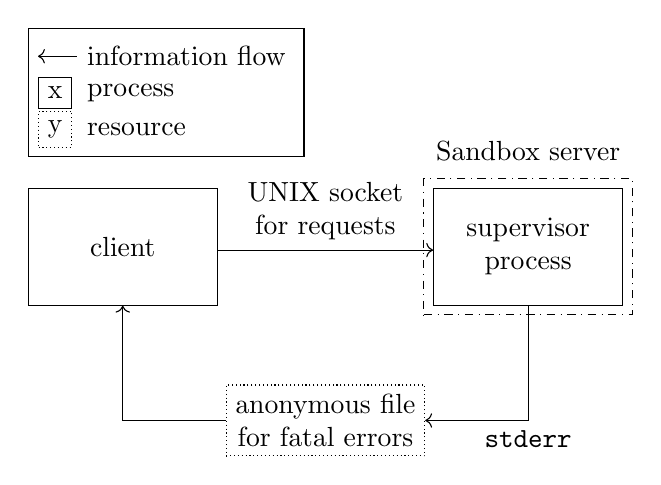
\begin{tikzpicture}[align=center]
    \node [draw, densely dotted] (errors) {anonymous file\\for fatal errors};
    \node [draw, above left=1cm and 0.1cm of errors, minimum height=1.4832815729996514cm, minimum width=2.4cm] (client) {client};
    \node [draw, above right=1cm and 0.1cm of errors, minimum height=1.4832815729996514cm, minimum width=2.4cm] (supervisor) {supervisor\\process};

    \draw[->] (client.-2) -- node[above] {UNIX socket \\ for requests} (supervisor.-178);
    \draw[<-] (client) |- node[below] {} (errors);
    \draw[->] (supervisor) |- node[below] {\texttt{stderr}} (errors);

    \begin{scope}[on background layer]
        \node [draw, dash dot, fit=(supervisor)] (server) {};
        \node [above=0.1cm of server] {Sandbox server};
    \end{scope}

    % Legend
    \matrix [draw, right] at ($(current bounding box.north west)+(0, 0.5)$) {
        \draw[<-] (0,0) -- (0.5,0); & \node[right] {information flow}; \\
        \draw node[right, draw] {x}; & \node[right] {process}; \\
        \draw node[right, draw, densely dotted] {y}; & \node[right] {resource}; \\
    };

\end{tikzpicture}
\caption{Sandbox server waits for requests. Client sends requests through the UNIX socket. Sandbox server will die on fatal error leaving the error message for the client in the anonymous file.}
\label{fig:server_waits_for_request}
\end{figure}

\subsection{Sandboxing request handling}

For each request, the server process (aka supervisor) spawns the PID 1 process of the new PID namespace. Then the init process setups namespaces and some of the resource limits. Finally the PID 1 process spawns the tracee process that finishes configuration and executes the requested executable. So for each sandboxing request we spawn exactly 2 processes. However, the executed program can spawn new processes --- each of them is referred to as a "tracee process". The PID 1 process is necessary for a couple of reasons:
\begin{itemize}
    \item It reaps the zombie processes in the tracee PID namespace.
    \item It allows locking mount-points in the mount namespace. The tracee process is spawned in a new user and mount namespace. Mounts are performed by the PID 1 process, therefore all mounts become locked together and cannot be individually unmounted by the tracee \cite{man_mount_namespaces}. These mounts cannot be performed by the supervisor process instead, because it would alter the mount namespace for subsequent requests.
    \item Inside a PID namespace, sending signals to the PID 1 process is allowed only for signals that the PID 1 process installed signal handler for. This could change the behavior for some programs, therefore a helper PID 1 process is needed.
\end{itemize}

This is shown on Figure \ref{fig:server_handles_request_after_execve}.

\begin{figure}[h]
\tikzset{>=latex} % set latex arrow tip
\centering
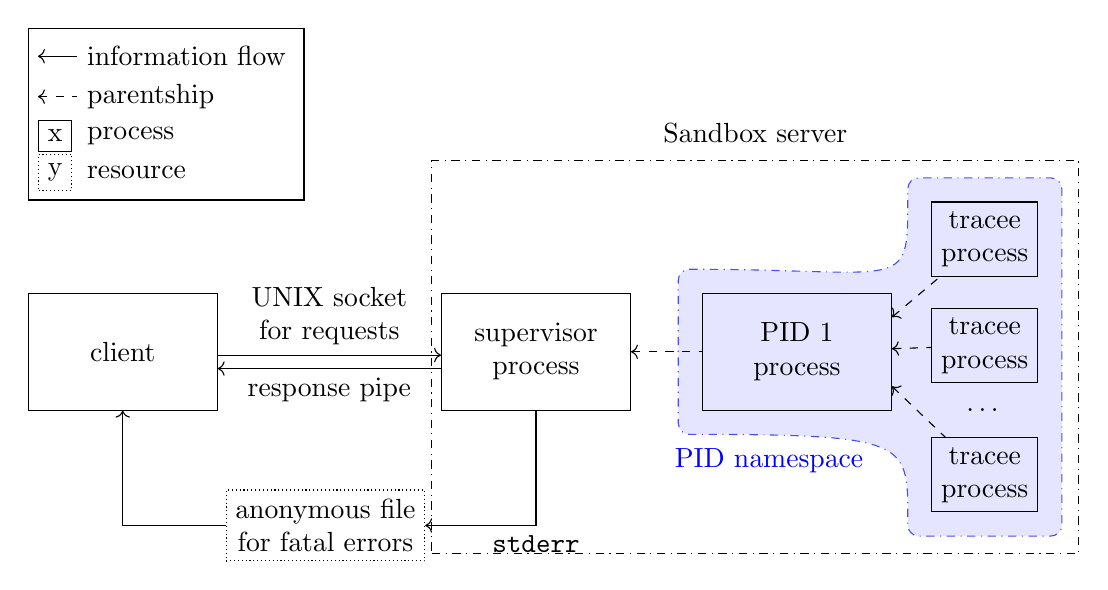
\begin{tikzpicture}[align=center]
    \node [draw, densely dotted] (errors) {anonymous file\\for fatal errors};
    \node [draw, above left=1cm and 0.1cm of errors, minimum height=1.4832815729996514cm, minimum width=2.4cm] (client) {client};
    \node [draw, above right=1cm and 0.2cm of errors, minimum height=1.4832815729996514cm, minimum width=2.4cm] (supervisor) {supervisor\\process};

    \node [draw, right=0cm and 0.9cm of supervisor, minimum height=1.4832815729996514cm, minimum width=2.4cm] (pid1) {PID 1\\process};

    \node [draw, above right=-0.4cm and 0.5cm of pid1.east] (tracee_mid) {tracee\\process};
    \node [draw, above=0.4cm of tracee_mid] (tracee_up) {tracee\\process};
    \node [below=0.2cm of tracee_mid] (tracee_dots) {\ldots};
    \node [draw, below=0.2cm of tracee_dots] (tracee_bottom) {tracee\\process};

    \draw[->] (client.-2) -- node[above] {UNIX socket \\ for requests} (supervisor.-178);
    \draw[<-] (client.-10) -- node[below] {response pipe} (supervisor.-170);
    \draw[<-] (client) |- node[below] {} (errors);
    \draw[->] (supervisor) |- node[below] {\texttt{stderr}} (errors);
    \draw[<-, dashed] (supervisor) -- (pid1);
    \draw[<-, dashed] (pid1) -- (tracee_mid);
    \draw[<-, dashed] (pid1.20) -- (tracee_up);
    \draw[<-, dashed] (pid1.-20) -- (tracee_bottom);

    \begin{scope}[on background layer]
        \draw [dash dot, rounded corners, blue!70, fill=blue!10]
            ($(pid1.north west)+(-0.3,0.3)$) .. controls +(0:3cm) and +(270:1.5cm) ..
            ($(tracee_up.north west)+(-0.3,0.3)$) --
            ($(tracee_up.north east)+(0.3,0.3)$) --
            ($(tracee_bottom.south east)+(0.3,-0.3)$) --
            ($(tracee_bottom.south west)+(-0.3,-0.3)$) .. controls +(90:1.2cm) and +(0:3cm) .. node[below, xshift=-8mm, pos=0.7, blue] {PID namespace}
            ($(pid1.south west)+(-0.3,-0.3)$) --
            cycle;
    \end{scope}

    \begin{scope}[on background layer]
        \coordinate (top_right) at ($(tracee_up.north east)+(0.4,0.4)$);
        \coordinate (bottom_right) at ($(tracee_bottom.south east)+(0.4,-0.4)$);
        \node [draw, dash dot, fit=(supervisor) (pid1) (top_right) (bottom_right)] (server) {};
        \node [above=0.1cm of server] {Sandbox server};
    \end{scope}

    % Legend
    \matrix [draw, right] at (current bounding box.north west) {
        \draw[<-] (0,0) -- (0.5,0); & \node[right] {information flow}; \\
        \draw[<-, dashed] (0,0) -- (0.5,0); & \node[right] {parentship}; \\
        \draw node[right, draw] {x}; & \node[right] {process}; \\
        \draw node[right, draw, densely dotted] {y}; & \node[right] {resource}; \\
    };

\end{tikzpicture}
\caption{Sandbox server handles a request, at the moment after executing the requested executable. Sandbox server will die on fatal error leaving the error message for the client in the anonymous file. Sandbox server consist of the supervisor process and its child --- the PID 1 process that is spawned for each request. The PID 1 process performs a role of the init process in the PID namespace of the tracee processes.}
\label{fig:server_handles_request_after_execve}
\end{figure}

\section{Cgroups}

The server gains write access to cgroup hierarchy by being executed through \texttt{systemd-run -{}-user -{}-scope -{}-property=Delegate=yes -{}-collect}. It enables \texttt{pid}, \texttt{memory}, and \texttt{cpu} controllers for the below subgroups.

At startup, the server process creates the cgroup v2 hierarchy that looks as follows:
\begin{itemize}
    \item \texttt{/supervisor} --- cgroup of the supervisor process,
    \item \texttt{/pid1} --- cgroup of the pid1 process,
    \item \texttt{/tracee} --- cgroup of the tracee processes.
\end{itemize}
After creation of the hierarchy it places the supervisor process in its cgroup. Subsequent processes are placed in their cgroups by making use of \texttt{CLONE\_INTO\_CGROUP} flag.
\newline
\texttt{/tracee} cgroup allows:
\begin{itemize}
    \item Killing all tracee processes by writing 1 to \texttt{/tracee/cgroup.kill} file.
    \item Reading CPU user and CPU system time via \texttt{/tracee/cpu.stat} file.
    \item Reading peak memory usage via \texttt{/tracee/memory.peak} file.
    \item Setting process/tread number limit by writing \texttt{/tracee/pids.max}.
    \item Setting memory hard limit by writing \texttt{/tracee/memory.max}.
    \item Setting CPU usage limit by writing \texttt{/tracee/cpu.max}.
    \item Disabling PSI accounting to reduce the sandboxing overhead by writing 0 to \\\texttt{/tracee/cgroup.pressure} file.
\end{itemize}
\texttt{/tracee} cgroup needs to be deleted and recreated after each request to reset \texttt{/tracee/cpu.stat} and \texttt{/tracee/memory.peak} files.

\section{Linux namespaces}

Linux allows unprivileged users to create user namespaces only. However, after entering a new user namespace the process gains all privileges inside the namespace and can create other namespaces.
\newline
The supervisor process creates the following namespaces:
\begin{itemize}
    \item user namespace --- in order to create other namespaces and hide user ID and group ID,
    \item mount namespace --- to allow mounting detached cgroups v2 hierarchy,
    \item cgroup namespace --- to allow mounting detached cgroups v2 hierarchy,
    \item network namespace --- to disconnect every tracee from network devices, done once, as it is costly,
    \item IPC namespace --- to isolate every tracee from other processes' IPC, done once, for optimization,
    \item UTS namespace --- to isolate every tracee from host's hostname, done once, for optimization,
    \item time namespace --- to isolate every tracee from host's time namespace, done once, for optimization.
\end{itemize}
The pid1 process creates the following namespaces:
\begin{itemize}
    \item user namespace --- in order to create other namespaces and hide user ID and group ID,
    \item mount namespace --- to allow mounting requested mount-point hierarchy,
    \item PID namespace --- to isolate tracee from accessing other processes.
\end{itemize}
The tracee process creates the following namespaces:
\begin{itemize}
    \item user namespace --- in order to create other namespaces and hide user ID and group ID and lock the mount tree,
    \item mount namespace --- in lock the mount tree created by pid1.
\end{itemize}
The listed namespaces hierarchy is illustrated on Figure \ref{fig:server_namespaces}.

\begin{figure}[h]
\tikzset{>=latex} % set latex arrow tip
\centering
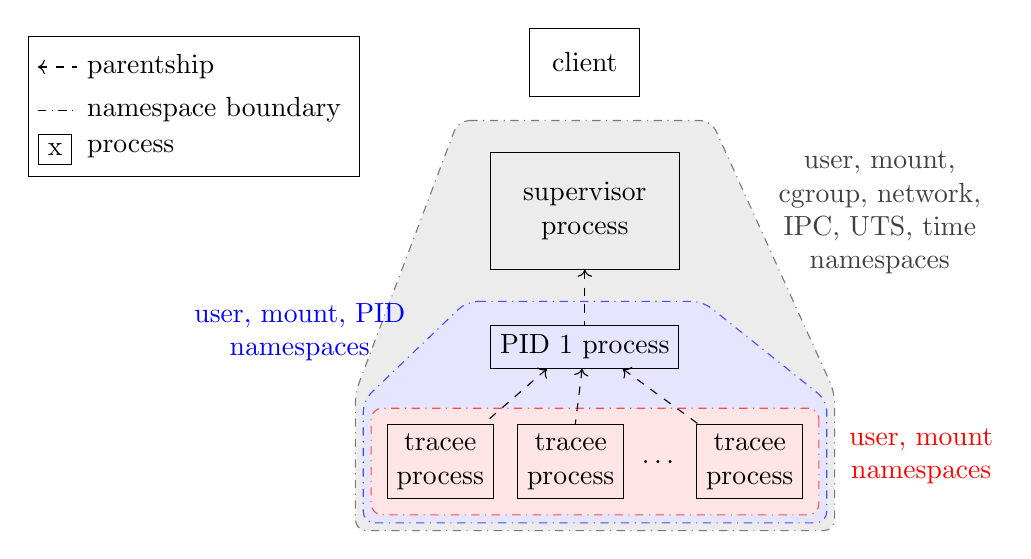
\begin{tikzpicture}[align=center]
    \node [draw, minimum height=0.8652475842497965cm, minimum width=1.4cm] (client) {client};

    \node [draw, below=0.7cm of client, minimum height=1.4832815729996514cm, minimum width=2.4cm] (supervisor) {supervisor\\process};

    \node [draw, below=0.7cm of supervisor] (pid1) {PID 1 process};

    \node [draw, below left=0.7cm and -1.7cm of pid1] (tracee_mid) {tracee\\process};
    \node [draw, left=0.3cm of tracee_mid] (tracee_left) {tracee\\process};
    \node [right=0.1cm of tracee_mid] (tracee_dots) {\ldots};
    \node [draw, right=0.1cm of tracee_dots] (tracee_right) {tracee\\process};

    \draw[<-, dashed] (supervisor) -- (pid1);
    \draw[<-, dashed] (pid1) -- (tracee_mid);
    \draw[<-, dashed] (pid1.-150) -- (tracee_left);
    \draw[<-, dashed] (pid1.-30) -- (tracee_right);

    \begin{scope}[on background layer]
        \draw[dash dot, rounded corners, darkgray!70, fill=darkgray!10]
            ($(supervisor.north west)+(-0.4,0.4)$) --
            ($(supervisor.north east)+(0.4,0.4)$) -- node[above, xshift=12mm, pos=0.6, darkgray] {user, mount,\\cgroup, network,\\IPC, UTS, time\\namespaces}
            ($(tracee_right.north east)+(0.4,0.4)$) --
            ($(tracee_right.south east)+(0.4,-0.4)$) --
            ($(tracee_left.south west)+(-0.4,-0.4)$) --
            ($(tracee_left.north west)+(-0.4,0.4)$) --
            cycle;
    \end{scope}

    \begin{scope}[on background layer]
        \draw[dash dot, rounded corners, blue!70, fill=blue!10]
            ($(pid1.north west)+(-0.3,0.3)$) --
            ($(pid1.north east)+(0.3,0.3)$) --
            ($(tracee_right.north east)+(0.3,0.3)$) --
            ($(tracee_right.south east)+(0.3,-0.3)$) --
            ($(tracee_left.south west)+(-0.3,-0.3)$) --
            ($(tracee_left.north west)+(-0.3,0.3)$) -- node[above, xshift=-12mm, pos=0.3, blue] {user, mount, PID\\namespaces}
            cycle;
    \end{scope}

    \begin{scope}[on background layer]
        \draw[dash dot, rounded corners, red!70, fill=red!10]
            ($(tracee_right.north east)+(0.2,0.2)$) -- node[above, xshift=13mm, pos=0.8, red] {user, mount\\namespaces}
            ($(tracee_right.south east)+(0.2,-0.2)$) --
            ($(tracee_left.south west)+(-0.2,-0.2)$) --
            ($(tracee_left.north west)+(-0.2,0.2)$) --
            cycle;
    \end{scope}

    % Legend
    \matrix [draw, right] at ($(current bounding box.north west)+(-2, -1)$) {
        \draw[<-, dashed] (0,0) -- (0.5,0); & \node[right] {parentship}; \\
        \draw[-, dash dot] (0,0) -- (0.5,0); & \node[right] {namespace boundary}; \\
        \draw node[right, draw] {x}; & \node[right] {process}; \\
    };

\end{tikzpicture}
\caption{Namespaces hierarchy of the sandbox server processes.}
\label{fig:server_namespaces}
\end{figure}

\section{Inter-process communication}

The client sends requests via UNIX domain socket to the supervisor process. The results are sent via a pipe attached to the request. The pipe is attached to the request as a file descriptor using \texttt{SCM\_RIGHTS} control message \cite{man_unix}.

The supervisor, pid1 and tracee process communicate via shared anonymous memory page. Figure \ref{fig:server_handles_request_before_execveat} illustrates this communication. Such communication requires no syscalls, is fast and reliable. This page is automatically unmapped upon \texttt{execveat} syscall \cite{man_execveat} in the tracee process, so it is protected from the tracee access.

\begin{figure}[h]
\tikzset{>=latex} % set latex arrow tip
\centering
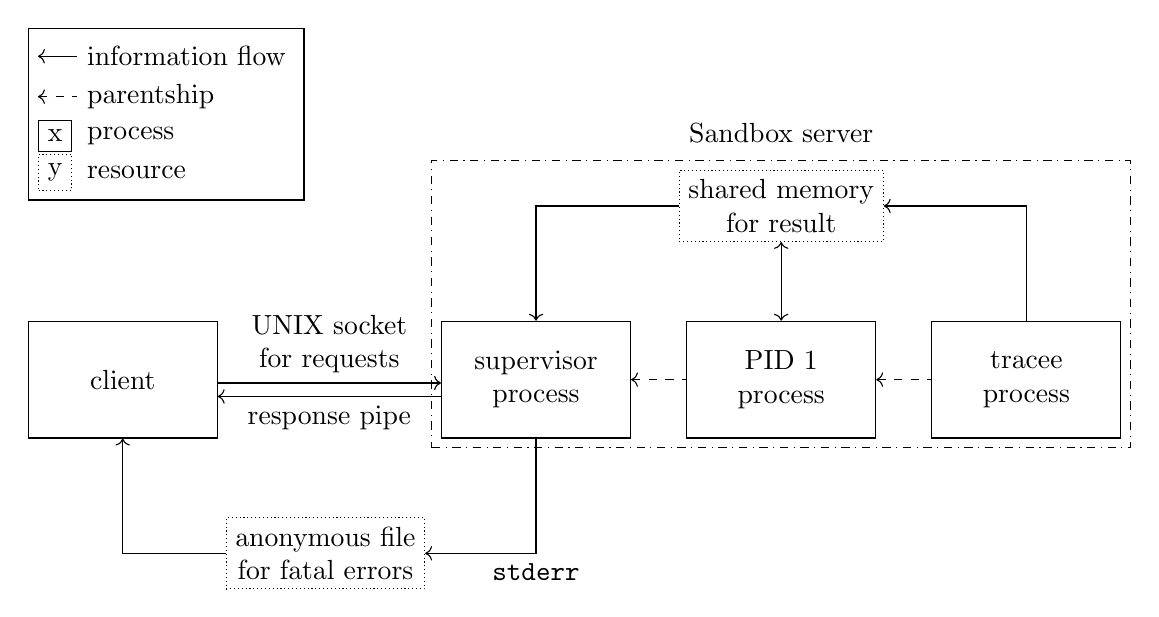
\begin{tikzpicture}[align=center]
    \node [draw, densely dotted] (errors) {anonymous file\\for fatal errors};
    \node [draw, above left=1cm and 0.1cm of errors, minimum height=1.4832815729996514cm, minimum width=2.4cm] (client) {client};
    \node [draw, above right=1cm and 0.2cm of errors, minimum height=1.4832815729996514cm, minimum width=2.4cm] (supervisor) {supervisor\\process};

    \node [draw, right=0cm and 0.7cm of supervisor, minimum height=1.4832815729996514cm, minimum width=2.4cm] (pid1) {PID 1\\process};

    \node [draw, right=0cm and 0.7cm of pid1, minimum height=1.4832815729996514cm, minimum width=2.4cm] (tracee) {tracee\\process};

    \node [draw, above=1cm of pid1, densely dotted] (shmem) {shared memory\\for result};

    \draw[->] (client.-2) -- node[above] {UNIX socket \\ for requests} (supervisor.-178);
    \draw[<-] (client.-10) -- node[below] {response pipe} (supervisor.-170);
    \draw[<-] (client) |- node[below] {} (errors);
    \draw[->] (supervisor) |- node[below] {\texttt{stderr}} (errors);
    \draw[<-] (supervisor.north) |- (shmem);
    \draw[<->] (shmem.south) -- (pid1.north);
    \draw[<-] (shmem.east) -| (tracee.north);
    \draw[<-, dashed] (supervisor) -- (pid1);
    \draw[<-, dashed] (pid1) -- (tracee);

    \begin{scope}[on background layer]
        \node [draw, dash dot, fit=(supervisor) (pid1) (shmem) (tracee)] (server) {};
        \node [above=0.1cm of server] {Sandbox server};
    \end{scope}

    % Legend
    \matrix [draw, right] at (current bounding box.north west) {
        \draw[<-] (0,0) -- (0.5,0); & \node[right] {information flow}; \\
        \draw[<-, dashed] (0,0) -- (0.5,0); & \node[right] {parentship}; \\
        \draw node[right, draw] {x}; & \node[right] {process}; \\
        \draw node[right, draw, densely dotted] {y}; & \node[right] {resource}; \\
    };

\end{tikzpicture}
\caption{Sandbox server handles a request, at the moment before executing the requested executable. Sandbox server will die on fatal error leaving the error message for the client in the anonymous file. Sandbox server consist of the supervisor process and its child --- the PID 1 process that is spawned for each request and its child --- the tracee process that will execute the requested executable. The tracee process saves in the shared memory the time just before \texttt{execveat} and signals the PID 1 process. The PID 1 process reads the time saved in the shared memory and starts the real and CPU timers. After the tracee process dies, the PID 1 process writes exit code and status of the tracee process and the time it died. Moreover, the shared memory is used to communicate fatal errors to the supervisor process.}
\label{fig:server_handles_request_before_execveat}
\end{figure}

\section{Capabilities}

The supervisor process drops all capabilities, sets securebits and \texttt{NO\_NEW\_PRIVS} flag. This ensures minimal possible capabilities in its and ancestor user namespace and prevents gaining any new privileges.

\section{Hardening}

The pid1 process, after spawning the tracee enters a new cgroup namespace to limit view of other namespaces i.e. if the tracee somehow takes control of the pid1 process, it will not be able to raise its PID and memory limit. Moreover a seccomp filter is installed to limit allowed syscalls only to those needed for reaping the orphaned zombie process, managing time limits and exiting upon tracee death.

\section{Conclusion}

Client-server architecture allows time-performance optimizations. Furthermore, it allows more common work to be done once and simplifies implementation. For instance, file descriptors do not leak to other processes because there are no threads that could fork a new process. Request handling requires creation of 2 processes --- the PID 1 process and the tracee process that later executes the requested program. Resource limits and accounting is mostly performed by cgroups. Isolation is achieved by deft usage of Linux namespaces.

\chapter{Implementation}\label{chapter:implementation}

The project is written in C++, as it is a low-overhead, low-level language, but more convenient than C. Git is used as a Version Control System to track incremental implementation. Invaluable tool used during development was \texttt{strace} \cite{strace}. It allowed easy inspection of system calls and their return values without any modification to the source code.

\section{Interface}

The client has to spawn the sandbox server --- the supervisor process. It then operates on the connection handle. Using the connection handle, the client can send requests to execute programs in the sandbox.

After sending a request, a request handle object is constructed. It can be used to obtain result of the execution, cancel execution or kill the tracee processes. Canceling execution is useful in case of errors in the client, where the result of the execution as well as the execution itself are no longer needed. Upon cancellation of the request, tracee process are immediately killed. Result of running the request is discarded. Canceling an already finished request discards the result. Canceling the request before the server started handling it causes it to be skipped. Killing an already finished request is no-op. Killing the request before the server started handling it causes tracee to be immediately killed after the \texttt{execveat}.

The client can then await the result of the request using the request handle. The result can either be a successful result or an error with a textual description. This error is not fatal to the supervisor process i.e. new requests can be sent. The successful result consists of the exit code and status, and runtime statistics:
\begin{itemize}
    \item real time,
    \item CPU user and CPU system time,
    \item peak tracee cgroup memory usage.
\end{itemize}
Each request has a set of accompanying options:
\begin{itemize}
    \item Optional \texttt{stdin}, \texttt{stdout}, and \texttt{stderr} file descriptors. If optional is specified as empty, \texttt{/dev/null} is opened as the file descriptor.
    \item Environment as an array view of string views.
    \item Linux namespace configuration:
        \begin{itemize}
            \item user ID and group ID mapping,
            \item mounts and new root mount,
        \end{itemize}
    \item Cgroup resource limits: process and thread limit, memory limit, CPU maximum bandwidth.
    \item \texttt{prlimit} hard limits.
    \item Real time limit.
    \item CPU time limit.
    \item Seccomp BPF filter as a file descriptor. The decision to pass it as a file descriptor is that it lowers the overhead of repeatedly using the same filter --- a common scenario in a judge system. Only the file descriptor needs to be sent with each request instead of the whole BPF filter content. This allows the filter to be compiled once and passed for multiple requests with minimal overhead. An alternative is to extend the API to save seccomp filters but it was considered unnecessary given how small is the overhead of passing a single file descriptor.
\end{itemize}

\section{Time limits}

The PID 1 process controls the time limits. The tracee process, just before \texttt{execveat} saves current real time from \texttt{CLOCK\_MONOTONIC\_RAW} and CPU time from \texttt{cpu.stat} tracee cgroup file to the shared memory (see Figure \ref{fig:server_handles_request_before_execveat}). The problem with \texttt{cpu.stat} file is that it is updated infrequently. For a young tracee process, this file often reports consumed CPU time equal to 0 microseconds instead of a few hundred microseconds. Fortunately, executing \texttt{sched\_yield()} system call forces recalculation of the file and the values are no longer 0. This is why this syscall is required as allowed in the seccomp BPF filter.

\subsection{Real time limit}

After saving the current real time the tracee process signals the PID 1 process with \texttt{SIGUSR2}. The PID 1 process reads the saved real time and sets up a POSIX timer to expire at the moment of saved time + real time limit. When the timer expires, \texttt{SIGUSR1} is sent by the kernel to the PID 1 process and it terminates all tracee processes by writing 1 to the \texttt{cgroup.kill} file of the tracee cgroup.

\subsection{CPU time limit}

In case the tracee is not restricted to one process, the setup is analogous to real time except that there is no CPU timer for a cgroup of processes. Instead we calculate minimal period of time in which the CPU time limit could expire as follows: $\frac{\text{remaining cpu time}}{\text{max parallelism}}$, where max parallelism equals: $\min(\text{available threads}, \text{\texttt{process\_num\_limit}}, \text{\texttt{cpu\_max\_bandwidth} in threads})$. Upon the timer expiration the remaining cpu time is recalculated and the timer is rescheduled if the remaining cpu time is greater than 0. Timer expiration is signaled by the kernel as signal \texttt{SIGXCPU}. To prevent polling, the minimal timer expiration period is capped to have minimum value of 1ms --- this gives at most 1000 checks per second.

In case the tracee is restricted to one process, the setup is different. After saving the current CPU time the tracee process signals the PID 1 process through a pipe. A signal cannot be used because \texttt{timer\_create} syscall and \texttt{clock\_getcpuclockid} library function are not marked async-signal-safe --- they are not specified to be safe to call inside a signal handler. An \texttt{eventfd} cannot be used either, because if tracee dies before writing to the \texttt{eventfd}, the PID 1 process will wait indefinitely on the \texttt{read} syscall. With a pipe, \texttt{read} syscall returns 0 when the other end becomes closed. With the limit of one process we use the CPU timer of the tracee process and set up a timer to expire when the tracee exceeds the CPU time limit.

In both cases, when the CPU time limit is exceeded, the PID 1 process is signaled about it and it terminates all tracee processes by writing 1 to \texttt{cgroup.kill} file of the tracee cgroup.

\section{Runtime statistics}

After the main tracee process (the first spawned process) exits, the PID 1 process saves the current real time and the exit status in the shared memory, unless the tracee set an error, and exits. The kernel kills all remaining tracee processes (because the PID namespace's init process died). After the PID 1 process exits, the supervisor process reads the shared memory (see Figure \ref{fig:server_handles_request_before_execveat}). It checks if there is an error of either tracee or PID 1 process. If there is one, it becomes the result of the request. If there is none, the supervisor process calculates:
\begin{itemize}
    \item real time using formula: $\text{time of tracee death} - \text{saved \texttt{execveat} real time}$,
    \item CPU time using formula: $\text{CPU time read from \texttt{cpu.stat} file} - \text{saved \texttt{execveat} CPU time}$,
    \item Peak memory usage by reading \texttt{memory.peak} tracee cgroup file.
\end{itemize}

\section{Error handling}

Errors in the supervisor process are considered fatal and are reported by writing to \texttt{stderr}. After writing errors, the supervisor process exits immediately. When the client tries to read the request result, the read will fail with \texttt{read} returning unexpected value 0. The client then ensures the supervisor process is dead (in case the communication failed) and tries to read the error the supervisor wrote. If the client finds one it throws exception with this error, otherwise it throws the exception with the \texttt{read} error.

The PID 1 process and tracee process write error to the shared memory (see Figure \ref{fig:server_handles_request_before_execveat}) and exit immediately. The supervisor process reports these errors as a request result.

\section{Request sending and receiving}

The request is sent via UNIX domain socket (see Figure \ref{fig:server_waits_for_request}). The request consists of a constant-length with file descriptors and a variable length body. The request header contains only the length of the request body. The request body contains all parameters of the request that are serialized to a custom binary format.

\section{File descriptors}

The sandbox server closes all file descriptors except the UNIX socket fd and opens \texttt{/dev/null} as \texttt{stdin}, \texttt{stdout}, and \texttt{stderr}. This is a small optimization, in case the request does not specify a standard file descriptor. For instance, if the request is to execute a program without \texttt{stdin}, the sandbox server has to set up the \texttt{stdin} of the tracee process to be \texttt{/dev/null} opened for reading. However, the tracee process inherits the file descriptors of the PID 1 process that inherits the file descriptors of the supervisor process. The supervisor process has already opened \texttt{/dev/null} as the \texttt{stdin} file descriptor. Therefore no action is needed in the PID 1 process and the tracee process for \texttt{stdin} of the tracee process to be \texttt{/dev/null} opened for reading. The same principle applies to \texttt{stdout} and \texttt{stderr} file descriptors.

All file descriptors are opened with \texttt{O\_CLOEXEC} flag so that they will not leak to the executed process. A unit test to check if any file descriptor leaks to the sandboxed program is in the test suite.

The PID 1 process inherits all request standard file descriptors and passes them to the tracee process. It has to close them after spawning the tracee process. To see why, let's consider a pipe of which one end is passed as a \texttt{stdin} to the sandboxed program. A pipe is broken if all file descriptors of one end become closed. If the PID 1 process did not close the standard file descriptors of the tracee, the pipe could not become broken until the PID 1 process dies. This changes the semantics of the pipe if the program is run inside the sandbox and is undesirable. Moreover, for hardening purposes the PID 1 process closes all unnecessary file descriptors after spawning tracee --- in case, the tracee somehow takes control of the PID 1 process.

\section{Canceling the request}

The response to the request is passed via pipe that is provided alongside the request. If the pipe becomes broken i.e. the client closes the read end of the pipe, the request is considered cancelled and is immediately discarded if currently handled and omitted otherwise.

\section{Killing the request}

Alongside request is send an \texttt{eventfd} file descriptor. The supervisor process monitors this file descriptor and if it becomes readable i.e. the client writes a value to it, the tracee is killed immediately. To avoid false-positive errors (the tracee process is killed unexpectedly), if the request is killed before \texttt{execveat} syscall executing the requested program, killing of the tracee is delayed to the \texttt{execve} moment.

\section{Sandbox server upon client death}

The supervisor process monitors the UNIX socket through which the requests flow in. If the other end becomes read and write closed, the supervisor recognises it as a death of the client process and dies immediately. The PID 1 process is configured to die upon the supervisor process death, and the kernel kills all tracee processes when the PID 1 process dies. Therefore, all server processes die.

\section{PID 1 process upon supervisor death}

The PID 1 process configures kernel to kill it upon the supervisor process death. This is done using \texttt{prctl}'s option \texttt{PR\_SET\_PDEATHSIG}. However, if the supervisor dies before the kernel configures the PID 1 process to die, the PID 1 process will still be alive and waste the resources. To solve this, one could check if the \texttt{getppid()} returns the expected PID of the supervisor process. However, this will not work, since the PID 1 process is in a new PID namespace, and \texttt{getppid()} will always return 0. A reliable solution is to pass a pidfd file descriptor of the supervisor process and check if the supervisor process is dead by checking if the pidfd file descriptor became readable. This way, upon supervisor process death, the PID 1 process is either killed by the kernel or it detects the death of the supervisor process and kills itself.

\section{Signals}

Signals are another way the processes can communicate with each other. They have their nuances and have to be isolated as well.

\subsection{Tracee signals}

Tracee can signal only to the visible processes and those are limited by the PID namespace. However, it can also send signals to its process group that can span multiple PID namespaces. Figure \ref{fig:pgid_and_pid_namespace} illustrates this situation. Therefore it is necessary to set new process group for the tracee processes. Furthermore, as a hardening, a new process group is set for the PID 1 process as well, in case the tracee takes control of it.

However, it is better to also set a new session id using \texttt{setsid} syscall instead of just the process group id to avoid vulnerabilities connected to the current controlling terminal \cite{bubblewrap_cve}.

\begin{figure}[h]
\tikzset{>=latex} % set latex arrow tip
\centering
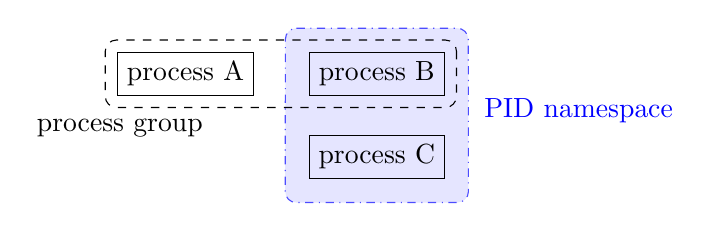
\begin{tikzpicture}[align=center]
    \node [draw] (a) {process A};
    \node [draw, right=0.7cm of a] (b) {process B};
    \node [draw, below=0.5cm of b] (c) {process C};

    \begin{scope}[on background layer]
        \draw[dash dot, rounded corners, blue!70, fill=blue!10]
            ($(b.north west)+(-0.3,0.3)$) --
            ($(b.north east)+(0.3,0.3)$) -- node[above, xshift=14mm, pos=0.6, blue] {PID namespace}
            ($(c.south east)+(0.3,-0.3)$) --
            ($(c.south west)+(-0.3,-0.3)$) --
            cycle;
    \end{scope}

    \begin{scope}[on background layer]
        \draw[dashed, rounded corners]
            ($(b.north east)+(0.15,0.15)$) --
            ($(b.south east)+(0.15,-0.15)$) -- node[above, yshift=-5mm, xshift=-16mm, pos=0.6] {process group}
            ($(a.south west)+(-0.15,-0.15)$) --
            ($(a.north west)+(-0.15,0.15)$) --
            cycle;
    \end{scope}

\end{tikzpicture}
\caption{Process group can span multiple PID namespaces.}
\label{fig:pgid_and_pid_namespace}
\end{figure}

\subsection{\texttt{SIGPIPE} in the supervisor process}

Sending response to the client may generate \texttt{SIGPIPE} signal for the supervisor process if the client cancels the request approximately in the same moment. We have to ignore this signal in the supervisor process. However, this cannot be done using \texttt{SIG\_IGN} because this signal disposition is not reset upon \texttt{execveat} system call and it had to be reset manually. As an alternative, it was chosen to install an empty signal handler for \texttt{SIGPIPE} so that the disposition of the signal handler is reset upon \texttt{execveat} in the tracee process automatically by the kernel.

\subsection{Undefined Behavior Sanitizer}

The code of the sandbox may be compiled with the Undefined Behavior Sanitizer (UBSan) enabled. UBSan installs signal handlers for \texttt{SIGBUS}, \texttt{SIGFPE} and \texttt{SIGSEGV} signals. This is problematic, because tracee could send these signals to the PID 1 process. For the init process in the PID namespace, the kernel only allows sending signals for which the init process (here the PID 1 process) has installed the signal handlers \cite{man_pid_namespaces}. Therefore the PID 1 process resets signal dispositions of these handlers if the UBSan is used to prevent tracee from sending these signals to the PID 1 process.

\section{Running as superuser}

The sandbox is not safe to be run by the superuser. If this is needed, then you have to switch to some unprivileged user first. This is because many global system resources are still available, even after dropping the capabilities, e.g. rising privileges works. The check is done in the supervisor process at startup. To make it user namespace-proof it is checked if \texttt{/dev/null} is the null device and if the effective user id of the process equals the owner of the \texttt{/dev/null} file.

\section{Performance optimizations}

Everything that can be done is done in the supervisor process at startup, before handling requests e.g. creating cgroups, entering the network namespace, opening \texttt{/dev/null} as standard file descriptors. Sharing this work between requests ensures minimal overhead of handling the request i.e. it increases throughput (handled requests per second). Some of the optimizations are described in this section.

\subsection{Seccomp filter of the PID 1 process}

The seccomp filter of the PID 1 process is created and compiled in the supervisor process. Therefore it is done once instead of for every request.

\subsection{Seccomp filter as file descriptor}

The seccomp filter in a request is sent as a file descriptor. This avoids unnecessary copies of the seccomp filter contents in case the filter is large. Moreover, the gain is more evident if the same filter is used for subsequent requests.

\subsection{Unsharing network, ipc, uts and time namespace}

Unsharing of network, ipc, uts and time namespace is done in the supervisor process, only once, at startup. This avoids doing it for every request in the PID 1 process and has non-negligible impact on the performance (see Chapter \ref{chapter:performance}).

\section{Integration with Online Judge Platform}

To integrate the new sandbox with the Online Judge Platform, a suite for each language was needed. The suite sandboxes the compiler if the language is compiled and sandboxes the runtime of the tested program. The following suites were implemented:

\begin{itemize}
    \item C, C++, Pascal and Rust --- fully compiled languages, the suite has to sandbox the compilation process and a fully compiled executable.
    \item Python, Bash --- fully interpreted languages, the suite does not have a compilation stage, but requires sandboxing the interpreter when it runs the solution.
\end{itemize}
The Bash language is used only for testing due to its short start-up time.

Each of the compilation and run stages requires creating a root file system and a seccomp BPF filter. Root file system has to include the following bind mounts (due to dynamically linked executables):
\begin{itemize}
    \item \texttt{/lib}
    \item \texttt{/lib64}
    \item \texttt{/usr/lib}
    \item \texttt{/usr/lib64}
\end{itemize}

Additionally, C, and C++ compilers require \texttt{/usr/bin} and \texttt{/usr/include}.
Pascal compiler requires \texttt{/usr/bin} and \texttt{/tmp}.
Rust compiler requires \texttt{/usr/bin}, \texttt{/tmp}, and on Debian \texttt{/proc}.
Bash and Python require no additional bind mounts.

\subsection{Interactive problems}

Interactive problems require the tested program to communicate with the checker program i.e. the standard input of the tested program is the standard output of the checker program and the standard output of the tested program is the standard input of the checker program. Figure \ref{fig:intaractive_problem_communication_schema} illustrates this configuration. To accomplish this we need two pipes, one for each communication channel. However, the judge needs to know which process died first to provide a reasonable verdict of checking the tested program on the test.

To see why, lets consider the two examples. In the first one, the checker decides early that the tested program answered wrong, it terminates with a message ''Wrong answer''. Then, the pipe closes and the tested program may get terminated by \texttt{SIGPIPE} for trying to write to the closed pipe. If this happens, the tested program's abnormal death is caused by the checker exiting early. In this situation verdict ''Wrong answer'' is the expected verdict. In the second example, an incorrect tested program terminates early and abnormally. In this case, the pipe closes after tested program's death and the checker sees the output of the tested program as incomplete and decides ''Wrong answer''. However, in this example an expected verdict would be ''Runtime error'' because the tested program's death caused checker to decide ''Wrong answer'', therefore tested program's abnormal death takes precedence here. If we don't know who died first in such cases, we cannot reliably deduce the primary cause and therefore cannot decide what is more important, a tested program's abnormal death or the checker's verdict.

\begin{figure}[h]
\tikzset{>=latex} % set latex arrow tip
\centering
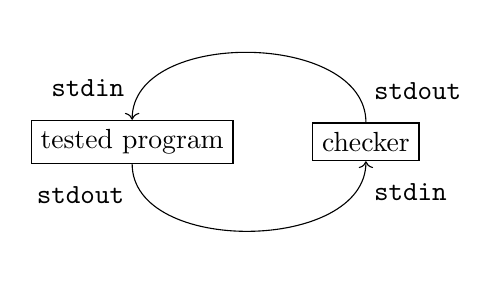
\begin{tikzpicture}[align=center]
    \coordinate (center) at (0,0);
    \node [draw, left=0.5cm of center] (tested_program) {tested program};
    \node [draw, right=0.5cm of center] (checker) {checker};

    \draw[->] (checker.north) to [out=90, in=90] node[pos=0.05, above right] {\texttt{stdout}} node[pos=0.95, above left] {\texttt{stdin}} (tested_program.north);
    \draw[->] (tested_program.south) to [out=-90, in=-90] node[pos=0.05, below left] {\texttt{stdout}} node[pos=0.95, below right] {\texttt{stdin}} (checker.south);
\end{tikzpicture}
\caption{Schema of the communication between the tested program and the checker in an interactive problem.}
\label{fig:intaractive_problem_communication_schema}
\end{figure}

To solve this, one could monitor the ends of the two pipes and see which end closes first. This is possible with e.g. \texttt{poll} syscall. However, it is prone to a race condition because the process monitoring the ends of the pipes may be scheduled after the checker and the tested program process and see them as if they died at the same moment. For example, the tested program process dies abnormally, then checker decides ''Wrong answer'' and exits and only then the \texttt{poll} syscall returns reporting all ends of the pipes as closed without the information which closed first. To avoid this race condition and decide reliably 4 pipes are needed and a process that glues both pairs of pipes together and detects which end is closed first. Figure \ref{fig:interactive_problem_real_communication} illustrates this configuration. As long as, the third process holds open inner four ends of the pipe pairs, the tested program and the checker will not see their \texttt{stdin} and \texttt{stdout} as broken and will not proceed (to terminate, either normally or not). This way we can reliably detect who dies first and give a correct verdict in the scenarios where one's death causes the other's death. To efficiently pass messages in the third process, the \texttt{splice} syscall is used.

\begin{figure}[h]
\tikzset{>=latex} % set latex arrow tip
\centering
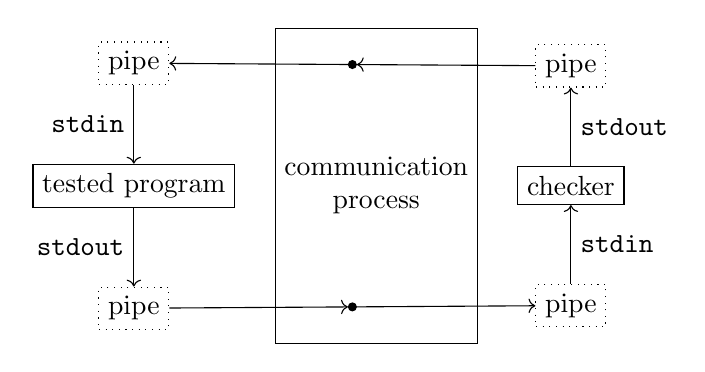
\begin{tikzpicture}[align=center]
    \node [draw, minimum height=4cm] (communicator) {communication\\process};
    \node [draw, left=0.5cm of communicator] (tested_program) {tested program};
    \node [draw, right=0.5cm of communicator] (checker) {checker};

    \node [draw, dotted, above=1cm of tested_program] (pipe_up_left) {pipe};
    \node [draw, dotted, below=1cm of tested_program] (pipe_down_left) {pipe};
    \node [draw, dotted, above=1cm of checker] (pipe_up_right) {pipe};
    \node [draw, dotted, below=1cm of checker] (pipe_down_right) {pipe};

    \node [draw, circle, fill=black, inner sep=0, minimum size=1mm] (up_dot) at ($(pipe_up_left)!.5!(pipe_up_right)$) {};
    \node [draw, circle, fill=black, inner sep=0, minimum size=1mm] (down_dot) at ($(pipe_down_left)!.5!(pipe_down_right)$) {};

    \draw[->] (tested_program) -- node[left] {\texttt{stdout}} (pipe_down_left);
    \draw[->] (pipe_down_left) -- (down_dot);
    \draw[->] (down_dot) -- (pipe_down_right);
    \draw[->] (pipe_down_right) -- node[right] {\texttt{stdin}} (checker);

    \draw[->] (checker) -- node[right] {\texttt{stdout}} (pipe_up_right);
    \draw[->] (pipe_up_right) -- (up_dot);
    \draw[->] (up_dot) -- (pipe_up_left);
    \draw[->] (pipe_up_left) -- node[left] {\texttt{stdin}} (tested_program);
\end{tikzpicture}
\caption{This is how communication between the tested program and the checker is implemented. Two pairs of pipes are used. This allows detection which process dies first --- the tested program or the checker. Because the communication process does not close its ends of the pipes first, it can detect which process died first without causing the second to die because of a broken pipe. To efficiently pass messages in the communication process, the \texttt{splice} syscall is used.}
\label{fig:interactive_problem_real_communication}
\end{figure}

\subsection{Non-interactive problems}

In the non-interactive problems, the semantics of the input is read-once and of the output is write-once. To achieve this without disallowing \texttt{dup}'ing, \texttt{close}'ing, \texttt{mmap}'ping, \texttt{pread}'ing etc. of the standard input and output file descriptors, we use pipes that are read-once and write-once. Input file is piped to \texttt{stdin} of the tested program, and the tested program's output is piped to the output file. Figure \ref{fig:noninteractive_problem_communication} illustrates this configuration. To efficiently pass messages between a pipe and a file the \texttt{splice} syscall is used.

\begin{figure}[h]
\tikzset{>=latex} % set latex arrow tip
\centering
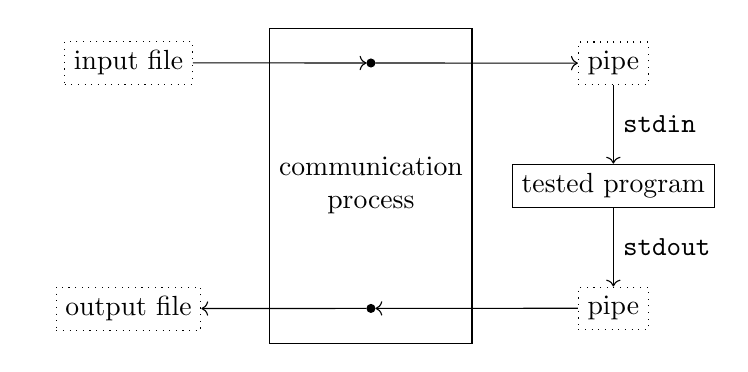
\begin{tikzpicture}[align=center]
    \node [draw, minimum height=4cm] (communicator) {communication\\process};
    \node [draw, right=0.5cm of communicator] (tested_program) {tested program};
    \node [left=0.5cm of communicator] (left_node) {\phantom{tested program}};

    \node [draw, dotted, above=1cm of left_node] (input_file) {input file};
    \node [draw, dotted, below=1cm of left_node] (output_file) {output file};
    \node [draw, dotted, above=1cm of tested_program] (pipe_up) {pipe};
    \node [draw, dotted, below=1cm of tested_program] (pipe_down) {pipe};

    \node [draw, circle, fill=black, inner sep=0, minimum size=1mm] (up_dot) at ($(input_file)!.5!(pipe_up)$) {};
    \node [draw, circle, fill=black, inner sep=0, minimum size=1mm] (down_dot) at ($(output_file)!.5!(pipe_down)$) {};

    \draw[->] (input_file) -- (up_dot);
    \draw[->] (up_dot) -- (pipe_up);
    \draw[->] (pipe_up) -- node[right] {\texttt{stdin}} (tested_program);
    \draw[->] (tested_program) -- node[right] {\texttt{stdout}} (pipe_down);
    \draw[->] (pipe_down) -- (down_dot);
    \draw[->] (down_dot) -- (output_file);
\end{tikzpicture}
\caption{To provide the read-once semantics of the standard input and the write-once semantics of the standard output the pipes are used. The communication process passes contents of the file to the input pipe that outputs to the tested program's \texttt{stdin}. The tested program's \texttt{stdout} is piped to the output file. To efficiently pass data between files and pipes in the communication process, the \texttt{splice} syscall is used.}
\label{fig:noninteractive_problem_communication}
\end{figure}

\subsection{Conclusion}

Apart from the above difficulties, the integration was rather easy. It required changing usage of the old sandbox to the new sandbox knobs. A lot of code was simplified along the way.

\section{Testing and validation}

To test and validate the new sandbox a comprehensive set of unit tests was developed. Tests check that namespaces are used appropriately, the interface is implemented correctly, the limits are enforced, runtime statistics are provided and are correct, no file descriptor leaks to the traced process, etc. Error reporting was also tested e.g. that unexpected supervisor death is reported, the supervisor terminates as soon as the socket connection with the client becomes broken etc. These tests ensured no regressions during the development and in the end eased the development process.

\section{Challenges faced}

There were many challenges during the development of the sandbox. First was to understand the semantics of the kernel's interfaces i.e. namespaces, cgroups and capabilities, and nuances in every one of them. One of the great achievements was to desist from using \texttt{ptrace} and all its complexity, while controlling a group of processes. This reduced the overhead and simplified things a lot. It was possible thanks to the Linux namespaces and cgroups.

Another challenge was to orchestrate everything to work together: resource limits, file descriptors, communication between processes, setting up namespaces and cgroups, dropping capabilities etc. It all has to be done in the right order and was often unobvious how to do it right.

The hardest of all was to debug very obscure errors happening during setup of the namespaces and cgroups. Often configuration failed with \texttt{EPERM} or \texttt{EINVAL} and it required figuring out what was wrong with just such vague information. For example, mounting cgroup2 file system is not allowed without unsharing cgroup namespace first. It also requires unsharing mount namespace and user namespace, but this is completely reasonable. In Sections \ref{execveat_returns_einval} and \ref{execveat_returns_enoent} two examples are shown of the hard to debug errors.

\subsection{\texttt{execveat} returns \texttt{EINVAL}} \label{execveat_returns_einval}

Executing a dynamically linked executable may fail with an error \texttt{EINVAL}. The executable needs the dynamic linker, so one reason of the error is the missing dynamic linker in the new root file system, on x86\_64 it is at \texttt{/lib64/ld-linux-x86-64.so.2}. Another reason may be a missing shared library that usually resides in the directory \texttt{/usr/lib/}. It is important to bind mount all of these paths during creation of the root file system for the dynamic executables to work.

\subsection{\texttt{execveat} returns \texttt{ENOENT}} \label{execveat_returns_enoent}

Executing a file may fail with \texttt{ENOENT}, even though the file exists. This may happen because the file is a symbolic link and the destination does not exist, or if the symbolic link is recursive (refers to a symbolic link) and one of the intermediate files is non-existent in the new root file system. One of the solutions is to bind mount the executable without \texttt{AT\_SYMLINK\_NOFOLLOW}.

\section{Conclusion}

Despite challenges and complexity the sandbox was implemented and tested successfully. The usage of Linux namespaces provides isolation while cgroups and prlimits limit the resources. The sandbox is versatile enough to be used both as a sandbox for running a tested program as well as for running the compiler. The goal of optimizing the implementation for short-running programs was achieved with several optimizations.


\chapter{Performance Evaluation}\label{chapter:performance}

All performance tests were made on a laptop with Intel i5-8250U processor and 16 GB of RAM. The purpose of this chapter is to verify the efficiency of the sandbox in the context of the online judge platform and briefly compare it with nsjail.

\section{In the context of the online judge}

For the testing we use tasks from the finale of XXII Polish Olimpiad in Informatics: Myjnie (myj), Tablice kierunkowe (tab), Modernizacja autostrady (mod), Wycieczki (wyc). The solutions programs are written by the problem package makers, they are used to verify the test cases will distinguish the different solutions of the users e.g. those running in $O(n)$ and $O(n^2)$. The model solution program is the main solution program that is the best solution program for the problem. In Polish it is called ''rozwiązanie wzorcowe''. The term ''solution'' can be misleading but is currently used in the English literature regarding Olympiads in Informatics \cite{kolstad2009infrastructure, marevs2012new, merry2010performance, merry2009using}.

First, we compare the compilation times of all solution programs outside sandbox, inside sandbox and inside sandbox with BPF filters disabled. Then we compare the running times of the model solution program of each problem.

\subsection{Compilation}

Table \ref{table:myj_compilation} contains the compilation times of solution programs of problem Myjnie.
Table \ref{table:tab_compilation} contains the compilation times of solution programs of problem Tablice kierunkowe.
Table \ref{table:mod_compilation} contains the compilation times of solution programs of problem Modernizacja autostrady.
Table \ref{table:wyc_compilation} contains the compilation times of solution programs of problem Wycieczki.

From the measurements we see that most of the overhead comes from BPF filters that cause up to 10\% slowdown. The compilation in the sandbox can be slower by up to 24\%, but can be also be faster by up to 12\%. We could not identify where the speedup comes from, it requires further investigation. Most of the time, the sandbox's slowdown is below 10\% compared to compilation time without the sandbox.

Commands used in testing:
\begin{itemize}
    \item C --- \texttt{/usr/bin/gcc -std=c11 -O2 -static -o exe source.c}. Compiler version: 13.2.1.
    \item C++ --- \texttt{/usr/bin/g++ -std=c++17 -O2 -static -o exe source.cc}. Compiler version: 13.2.1.
    \item Pascal --- \texttt{/usr/bin/fpc -O2 -XS -Xt -oexe source.pas}. Compiler version 3.3.2.
\end{itemize}

\newpage

\subsubsection{Myjnie (myj)}

\begin{small}
\begin{longtable}{|l|c|c|r|r|r|r|}
\hline
\makecell{Solution\\program} & Sandbox & Time & \makecell{Mean} & \makecell{Std. dev.} & \makecell{Std. err.\\on the mean} & \makecell{Slowdown} \\
\hline
\multirow{6}{*}{myj.cpp}    & \multirow{2}{*}{no}     & real & 362.60ms & 8.85ms (2.44\%) & 2.80ms (0.77\%) & 0.00\% \\*
                            &                         & CPU  & 356.96ms & 5.01ms (1.40\%) & 1.59ms (0.44\%) & 0.00\% \\*
                            \cline{2-7}
                            & \multirow{2}{*}{yes}    & real & 386.11ms & 7.27ms (1.88\%) & 2.30ms (0.60\%) & 6.48\% \\*
                            &                         & CPU  & 379.41ms & 6.12ms (1.61\%) & 1.93ms (0.51\%) & 6.29\% \\*
                            \cline{2-7}
                            & \multirow{2}{*}{no BPF} & real & 359.60ms & 6.73ms (1.87\%) & 2.13ms (0.59\%) & -0.83\% \\*
                            &                         & CPU  & 350.94ms & 5.31ms (1.51\%) & 1.68ms (0.48\%) & -1.69\% \\
\hline
\multirow{6}{*}{myj1.pas}   & \multirow{2}{*}{no}     & real & 72.18ms & 6.26ms (8.68\%) & 1.98ms (2.74\%) & 0.00\% \\*
                            &                         & CPU  & 69.66ms & 4.93ms (7.07\%) & 1.56ms (2.24\%) & 0.00\% \\*
                            \cline{2-7}
                            & \multirow{2}{*}{yes}    & real & 70.10ms & 4.26ms (6.07\%) & 1.35ms (1.92\%) & -2.87\% \\*
                            &                         & CPU  & 67.60ms & 3.52ms (5.21\%) & 1.11ms (1.65\%) & -2.96\% \\*
                            \cline{2-7}
                            & \multirow{2}{*}{no BPF} & real & 69.68ms & 5.00ms (7.17\%) & 1.58ms (2.27\%) & -3.46\% \\*
                            &                         & CPU  & 67.99ms & 5.09ms (7.48\%) & 1.61ms (2.37\%) & -2.39\% \\
\hline
\multirow{6}{*}{myj2.cpp}   & \multirow{2}{*}{no}     & real & 369.42ms & 7.44ms (2.01\%) & 2.35ms (0.64\%) & 0.00\% \\*
                            &                         & CPU  & 362.72ms & 4.64ms (1.28\%) & 1.47ms (0.40\%) & 0.00\% \\*
                            \cline{2-7}
                            & \multirow{2}{*}{yes}    & real & 388.42ms & 8.44ms (2.17\%) & 2.67ms (0.69\%) & 5.14\% \\*
                            &                         & CPU  & 377.39ms & 6.00ms (1.59\%) & 1.90ms (0.50\%) & 4.04\% \\*
                            \cline{2-7}
                            & \multirow{2}{*}{no BPF} & real & 352.86ms & 5.79ms (1.64\%) & 1.83ms (0.52\%) & -4.48\% \\*
                            &                         & CPU  & 348.17ms & 5.48ms (1.57\%) & 1.73ms (0.50\%) & -4.01\% \\
\hline
\multirow{6}{*}{myj3.cpp}   & \multirow{2}{*}{no}     & real & 394.17ms & 6.51ms (1.65\%) & 2.06ms (0.52\%) & 0.00\% \\*
                            &                         & CPU  & 384.30ms & 5.93ms (1.54\%) & 1.88ms (0.49\%) & 0.00\% \\*
                            \cline{2-7}
                            & \multirow{2}{*}{yes}    & real & 404.30ms & 6.35ms (1.57\%) & 2.01ms (0.50\%) & 2.57\% \\*
                            &                         & CPU  & 396.11ms & 5.26ms (1.33\%) & 1.66ms (0.42\%) & 3.07\% \\*
                            \cline{2-7}
                            & \multirow{2}{*}{no BPF} & real & 378.24ms & 8.30ms (2.20\%) & 2.63ms (0.69\%) & -4.04\% \\*
                            &                         & CPU  & 373.52ms & 5.86ms (1.57\%) & 1.85ms (0.50\%) & -2.81\% \\
\hline
\multirow{6}{*}{myj4.cpp}   & \multirow{2}{*}{no}     & real & 2105.00ms & 32.27ms (1.53\%) & 10.20ms (0.48\%) & 0.00\% \\*
                            &                         & CPU  & 2083.61ms & 29.28ms (1.41\%) & 9.26ms (0.44\%) & 0.00\% \\*
                            \cline{2-7}
                            & \multirow{2}{*}{yes}    & real & 2244.82ms & 184.78ms (8.23\%) & 58.43ms (2.60\%) & 6.64\% \\*
                            &                         & CPU  & 2222.96ms & 183.39ms (8.25\%) & 57.99ms (2.61\%) & 6.69\% \\*
                            \cline{2-7}
                            & \multirow{2}{*}{no BPF} & real & 2093.29ms & 39.94ms (1.91\%) & 12.63ms (0.60\%) & -0.56\% \\*
                            &                         & CPU  & 2069.41ms & 32.68ms (1.58\%) & 10.33ms (0.50\%) & -0.68\% \\
\hline
\multirow{6}{*}{myjb1.cpp}  & \multirow{2}{*}{no}     & real & 366.94ms & 7.57ms (2.06\%) & 2.40ms (0.65\%) & 0.00\% \\*
                            &                         & CPU  & 359.89ms & 4.60ms (1.28\%) & 1.46ms (0.40\%) & 0.00\% \\*
                            \cline{2-7}
                            & \multirow{2}{*}{yes}    & real & 384.46ms & 6.89ms (1.79\%) & 2.18ms (0.57\%) & 4.77\% \\*
                            &                         & CPU  & 376.95ms & 5.20ms (1.38\%) & 1.65ms (0.44\%) & 4.74\% \\*
                            \cline{2-7}
                            & \multirow{2}{*}{no BPF} & real & 353.91ms & 8.68ms (2.45\%) & 2.74ms (0.78\%) & -3.55\% \\*
                            &                         & CPU  & 346.75ms & 4.14ms (1.19\%) & 1.31ms (0.38\%) & -3.65\% \\
\hline
\multirow{6}{*}{myjb2.cpp}  & \multirow{2}{*}{no}     & real & 334.10ms & 3.68ms (1.10\%) & 1.16ms (0.35\%) & 0.00\% \\*
                            &                         & CPU  & 329.16ms & 4.85ms (1.47\%) & 1.53ms (0.47\%) & 0.00\% \\*
                            \cline{2-7}
                            & \multirow{2}{*}{yes}    & real & 336.05ms & 6.57ms (1.96\%) & 2.08ms (0.62\%) & 0.58\% \\*
                            &                         & CPU  & 328.03ms & 4.88ms (1.49\%) & 1.54ms (0.47\%) & -0.34\% \\*
                            \cline{2-7}
                            & \multirow{2}{*}{no BPF} & real & 321.29ms & 6.00ms (1.87\%) & 1.90ms (0.59\%) & -3.84\% \\*
                            &                         & CPU  & 314.97ms & 5.34ms (1.70\%) & 1.69ms (0.54\%) & -4.31\% \\
\hline
\multirow{6}{*}{myjb3.cpp}  & \multirow{2}{*}{no}     & real & 369.83ms & 6.01ms (1.63\%) & 1.90ms (0.51\%) & 0.00\% \\*
                            &                         & CPU  & 365.12ms & 7.22ms (1.98\%) & 2.28ms (0.63\%) & 0.00\% \\*
                            \cline{2-7}
                            & \multirow{2}{*}{yes}    & real & 380.30ms & 6.99ms (1.84\%) & 2.21ms (0.58\%) & 2.83\% \\*
                            &                         & CPU  & 373.70ms & 2.52ms (0.67\%) & 0.80ms (0.21\%) & 2.35\% \\*
                            \cline{2-7}
                            & \multirow{2}{*}{no BPF} & real & 351.72ms & 3.58ms (1.02\%) & 1.13ms (0.32\%) & -4.90\% \\*
                            &                         & CPU  & 346.07ms & 3.65ms (1.06\%) & 1.16ms (0.33\%) & -5.22\% \\
\hline
\multirow{6}{*}{myjb4.cpp}  & \multirow{2}{*}{no}     & real & 355.35ms & 8.39ms (2.36\%) & 2.65ms (0.75\%) & 0.00\% \\*
                            &                         & CPU  & 348.56ms & 6.47ms (1.86\%) & 2.05ms (0.59\%) & 0.00\% \\*
                            \cline{2-7}
                            & \multirow{2}{*}{yes}    & real & 364.72ms & 6.54ms (1.79\%) & 2.07ms (0.57\%) & 2.64\% \\*
                            &                         & CPU  & 358.57ms & 6.47ms (1.80\%) & 2.04ms (0.57\%) & 2.87\% \\*
                            \cline{2-7}
                            & \multirow{2}{*}{no BPF} & real & 343.04ms & 7.69ms (2.24\%) & 2.43ms (0.71\%) & -3.46\% \\*
                            &                         & CPU  & 333.60ms & 3.65ms (1.09\%) & 1.16ms (0.35\%) & -4.29\% \\
\hline
\multirow{6}{*}{myjb5.cpp}  & \multirow{2}{*}{no}     & real & 358.90ms & 8.32ms (2.32\%) & 2.63ms (0.73\%) & 0.00\% \\*
                            &                         & CPU  & 349.96ms & 8.32ms (2.38\%) & 2.63ms (0.75\%) & 0.00\% \\*
                            \cline{2-7}
                            & \multirow{2}{*}{yes}    & real & 370.24ms & 8.78ms (2.37\%) & 2.78ms (0.75\%) & 3.16\% \\*
                            &                         & CPU  & 362.40ms & 4.99ms (1.38\%) & 1.58ms (0.44\%) & 3.55\% \\*
                            \cline{2-7}
                            & \multirow{2}{*}{no BPF} & real & 342.85ms & 7.98ms (2.33\%) & 2.52ms (0.74\%) & -4.47\% \\*
                            &                         & CPU  & 336.04ms & 5.80ms (1.72\%) & 1.83ms (0.55\%) & -3.98\% \\
\hline
\multirow{6}{*}{myjs1.cpp}  & \multirow{2}{*}{no}     & real & 336.79ms & 31.10ms (9.23\%) & 9.83ms (2.92\%) & 0.00\% \\*
                            &                         & CPU  & 332.67ms & 29.36ms (8.83\%) & 9.29ms (2.79\%) & 0.00\% \\*
                            \cline{2-7}
                            & \multirow{2}{*}{yes}    & real & 338.45ms & 35.76ms (10.57\%) & 11.31ms (3.34\%) & 0.49\% \\*
                            &                         & CPU  & 330.57ms & 28.16ms (8.52\%) & 8.91ms (2.69\%) & -0.63\% \\*
                            \cline{2-7}
                            & \multirow{2}{*}{no BPF} & real & 356.88ms & 6.26ms (1.75\%) & 1.98ms (0.55\%) & 5.97\% \\*
                            &                         & CPU  & 348.74ms & 6.58ms (1.89\%) & 2.08ms (0.60\%) & 4.83\% \\
\hline
\multirow{6}{*}{myjs2.pas}  & \multirow{2}{*}{no}     & real & 69.89ms & 4.75ms (6.80\%) & 1.50ms (2.15\%) & 0.00\% \\*
                            &                         & CPU  & 68.40ms & 4.49ms (6.57\%) & 1.42ms (2.08\%) & 0.00\% \\*
                            \cline{2-7}
                            & \multirow{2}{*}{yes}    & real & 69.28ms & 5.55ms (8.02\%) & 1.76ms (2.53\%) & -0.86\% \\*
                            &                         & CPU  & 66.16ms & 5.26ms (7.95\%) & 1.66ms (2.51\%) & -3.28\% \\*
                            \cline{2-7}
                            & \multirow{2}{*}{no BPF} & real & 67.74ms & 5.00ms (7.39\%) & 1.58ms (2.34\%) & -3.07\% \\*
                            &                         & CPU  & 65.72ms & 4.25ms (6.46\%) & 1.34ms (2.04\%) & -3.92\% \\
\hline
\multirow{6}{*}{myjs3.cpp}  & \multirow{2}{*}{no}     & real & 369.35ms & 7.23ms (1.96\%) & 2.29ms (0.62\%) & 0.00\% \\*
                            &                         & CPU  & 360.47ms & 6.47ms (1.79\%) & 2.04ms (0.57\%) & 0.00\% \\*
                            \cline{2-7}
                            & \multirow{2}{*}{yes}    & real & 380.47ms & 7.97ms (2.09\%) & 2.52ms (0.66\%) & 3.01\% \\*
                            &                         & CPU  & 371.12ms & 6.12ms (1.65\%) & 1.93ms (0.52\%) & 2.95\% \\*
                            \cline{2-7}
                            & \multirow{2}{*}{no BPF} & real & 354.97ms & 7.63ms (2.15\%) & 2.41ms (0.68\%) & -3.89\% \\*
                            &                         & CPU  & 345.67ms & 6.99ms (2.02\%) & 2.21ms (0.64\%) & -4.11\% \\
\hline
\multirow{6}{*}{myjs4.pas}  & \multirow{2}{*}{no}     & real & 72.02ms & 4.68ms (6.50\%) & 1.48ms (2.05\%) & 0.00\% \\*
                            &                         & CPU  & 70.75ms & 4.86ms (6.87\%) & 1.54ms (2.17\%) & 0.00\% \\*
                            \cline{2-7}
                            & \multirow{2}{*}{yes}    & real & 69.31ms & 4.13ms (5.95\%) & 1.30ms (1.88\%) & -3.77\% \\*
                            &                         & CPU  & 67.67ms & 3.94ms (5.82\%) & 1.25ms (1.84\%) & -4.35\% \\*
                            \cline{2-7}
                            & \multirow{2}{*}{no BPF} & real & 61.85ms & 7.01ms (11.34\%) & 2.22ms (3.59\%) & -14.13\% \\*
                            &                         & CPU  & 60.24ms & 6.41ms (10.65\%) & 2.03ms (3.37\%) & -14.86\% \\
\hline
\multirow{6}{*}{myjs5.cpp}  & \multirow{2}{*}{no}     & real & 310.64ms & 23.84ms (7.67\%) & 7.54ms (2.43\%) & 0.00\% \\*
                            &                         & CPU  & 306.25ms & 17.21ms (5.62\%) & 5.44ms (1.78\%) & 0.00\% \\*
                            \cline{2-7}
                            & \multirow{2}{*}{yes}    & real & 384.98ms & 7.94ms (2.06\%) & 2.51ms (0.65\%) & 23.93\% \\*
                            &                         & CPU  & 380.27ms & 7.79ms (2.05\%) & 2.46ms (0.65\%) & 24.17\% \\*
                            \cline{2-7}
                            & \multirow{2}{*}{no BPF} & real & 358.36ms & 7.67ms (2.14\%) & 2.43ms (0.68\%) & 15.36\% \\*
                            &                         & CPU  & 351.52ms & 4.90ms (1.40\%) & 1.55ms (0.44\%) & 14.78\% \\
\hline
\multirow{6}{*}{myjs6.pas}  & \multirow{2}{*}{no}     & real & 71.69ms & 4.21ms (5.88\%) & 1.33ms (1.86\%) & 0.00\% \\*
                            &                         & CPU  & 70.00ms & 4.01ms (5.73\%) & 1.27ms (1.81\%) & 0.00\% \\*
                            \cline{2-7}
                            & \multirow{2}{*}{yes}    & real & 68.40ms & 4.09ms (5.98\%) & 1.29ms (1.89\%) & -4.58\% \\*
                            &                         & CPU  & 66.64ms & 3.65ms (5.48\%) & 1.15ms (1.73\%) & -4.81\% \\*
                            \cline{2-7}
                            & \multirow{2}{*}{no BPF} & real & 69.24ms & 4.16ms (6.00\%) & 1.31ms (1.90\%) & -3.41\% \\*
                            &                         & CPU  & 66.45ms & 3.33ms (5.02\%) & 1.05ms (1.59\%) & -5.08\% \\
\hline
\multirow{6}{*}{myjs7.cpp}  & \multirow{2}{*}{no}     & real & 2123.70ms & 40.65ms (1.91\%) & 12.85ms (0.61\%) & 0.00\% \\*
                            &                         & CPU  & 2109.31ms & 33.11ms (1.57\%) & 10.47ms (0.50\%) & 0.00\% \\*
                            \cline{2-7}
                            & \multirow{2}{*}{yes}    & real & 2451.10ms & 37.92ms (1.55\%) & 11.99ms (0.49\%) & 15.42\% \\*
                            &                         & CPU  & 2425.73ms & 28.52ms (1.18\%) & 9.02ms (0.37\%) & 15.00\% \\*
                            \cline{2-7}
                            & \multirow{2}{*}{no BPF} & real & 2131.85ms & 35.95ms (1.69\%) & 11.37ms (0.53\%) & 0.38\% \\*
                            &                         & CPU  & 2111.61ms & 36.11ms (1.71\%) & 11.42ms (0.54\%) & 0.11\% \\
\hline
\multirow{6}{*}{myjs8.cpp}  & \multirow{2}{*}{no}     & real & 2013.38ms & 150.21ms (7.46\%) & 47.50ms (2.36\%) & 0.00\% \\*
                            &                         & CPU  & 1997.83ms & 149.04ms (7.46\%) & 47.13ms (2.36\%) & 0.00\% \\*
                            \cline{2-7}
                            & \multirow{2}{*}{yes}    & real & 2411.73ms & 33.09ms (1.37\%) & 10.46ms (0.43\%) & 19.79\% \\*
                            &                         & CPU  & 2382.87ms & 31.90ms (1.34\%) & 10.09ms (0.42\%) & 19.27\% \\*
                            \cline{2-7}
                            & \multirow{2}{*}{no BPF} & real & 2070.14ms & 38.98ms (1.88\%) & 12.33ms (0.60\%) & 2.82\% \\*
                            &                         & CPU  & 2053.40ms & 38.97ms (1.90\%) & 12.32ms (0.60\%) & 2.78\% \\
\hline
\caption{Compilation times of all solution programs of the problem Myjnie (myj) from the finale of XXII Polish Olimpiad in Informatics. For each configuration (Solution program and Sandbox columns) the data was collected from 10 runs. Real and CPU times were collected from the same runs. Slowdown is measured form the times of configuration without sandbox.}
\label{table:myj_compilation}
\end{longtable}
\end{small}

\subsubsection{Tablice kierunkowe (tab)}

\begin{small}
\begin{longtable}{|l|c|c|r|r|r|r|}
\hline
\makecell{Solution\\program} & Sandbox & Time & \makecell{Mean} & \makecell{Std. dev.} & \makecell{Std. err.\\on the mean} & \makecell{Slowdown} \\
\hline
\multirow{6}{*}{tab.cpp}    & \multirow{2}{*}{no}     & real & 1502.95ms & 25.17ms (1.67\%) & 7.96ms (0.53\%) & 0.00\% \\*
                            &                         & CPU  & 1488.30ms & 20.63ms (1.39\%) & 6.52ms (0.44\%) & 0.00\% \\*
                            \cline{2-7}
                            & \multirow{2}{*}{yes}    & real & 1634.57ms & 18.91ms (1.16\%) & 5.98ms (0.37\%) & 8.76\% \\*
                            &                         & CPU  & 1609.73ms & 19.95ms (1.24\%) & 6.31ms (0.39\%) & 8.16\% \\*
                            \cline{2-7}
                            & \multirow{2}{*}{no BPF} & real & 1402.92ms & 105.52ms (7.52\%) & 33.37ms (2.38\%) & -6.66\% \\*
                            &                         & CPU  & 1389.83ms & 102.23ms (7.36\%) & 32.33ms (2.33\%) & -6.62\% \\
\hline
\multirow{6}{*}{tab2.c}     & \multirow{2}{*}{no}     & real & 222.52ms & 79.15ms (35.57\%) & 25.03ms (11.25\%) & 0.00\% \\*
                            &                         & CPU  & 192.33ms & 14.33ms (7.45\%) & 4.53ms (2.36\%) & 0.00\% \\*
                            \cline{2-7}
                            & \multirow{2}{*}{yes}    & real & 195.05ms & 4.84ms (2.48\%) & 1.53ms (0.79\%) & -12.34\% \\*
                            &                         & CPU  & 190.64ms & 3.50ms (1.84\%) & 1.11ms (0.58\%) & -0.88\% \\*
                            \cline{2-7}
                            & \multirow{2}{*}{no BPF} & real & 196.87ms & 4.45ms (2.26\%) & 1.41ms (0.72\%) & -11.53\% \\*
                            &                         & CPU  & 190.74ms & 2.57ms (1.35\%) & 0.81ms (0.43\%) & -0.83\% \\
\hline
\multirow{6}{*}{tab3.pas}   & \multirow{2}{*}{no}     & real & 75.84ms & 5.48ms (7.23\%) & 1.73ms (2.28\%) & 0.00\% \\*
                            &                         & CPU  & 72.71ms & 4.38ms (6.02\%) & 1.38ms (1.90\%) & 0.00\% \\*
                            \cline{2-7}
                            & \multirow{2}{*}{yes}    & real & 71.19ms & 3.61ms (5.07\%) & 1.14ms (1.60\%) & -6.14\% \\*
                            &                         & CPU  & 69.66ms & 3.18ms (4.56\%) & 1.00ms (1.44\%) & -4.20\% \\*
                            \cline{2-7}
                            & \multirow{2}{*}{no BPF} & real & 70.14ms & 5.72ms (8.16\%) & 1.81ms (2.58\%) & -7.53\% \\*
                            &                         & CPU  & 67.41ms & 4.27ms (6.34\%) & 1.35ms (2.00\%) & -7.30\% \\
\hline
\multirow{6}{*}{tab4.cpp}   & \multirow{2}{*}{no}     & real & 2261.35ms & 39.40ms (1.74\%) & 12.46ms (0.55\%) & 0.00\% \\*
                            &                         & CPU  & 2232.11ms & 33.15ms (1.49\%) & 10.48ms (0.47\%) & 0.00\% \\*
                            \cline{2-7}
                            & \multirow{2}{*}{yes}    & real & 2525.38ms & 62.24ms (2.46\%) & 19.68ms (0.78\%) & 11.68\% \\*
                            &                         & CPU  & 2503.59ms & 61.71ms (2.46\%) & 19.51ms (0.78\%) & 12.16\% \\*
                            \cline{2-7}
                            & \multirow{2}{*}{no BPF} & real & 2182.13ms & 43.47ms (1.99\%) & 13.75ms (0.63\%) & -3.50\% \\*
                            &                         & CPU  & 2154.98ms & 35.40ms (1.64\%) & 11.19ms (0.52\%) & -3.46\% \\
\hline
\multirow{6}{*}{tabb1.cpp}  & \multirow{2}{*}{no}     & real & 1631.92ms & 121.04ms (7.42\%) & 38.28ms (2.35\%) & 0.00\% \\*
                            &                         & CPU  & 1615.02ms & 120.35ms (7.45\%) & 38.06ms (2.36\%) & 0.00\% \\*
                            \cline{2-7}
                            & \multirow{2}{*}{yes}    & real & 1831.19ms & 33.72ms (1.84\%) & 10.66ms (0.58\%) & 12.21\% \\*
                            &                         & CPU  & 1813.79ms & 31.32ms (1.73\%) & 9.90ms (0.55\%) & 12.31\% \\*
                            \cline{2-7}
                            & \multirow{2}{*}{no BPF} & real & 1679.20ms & 23.03ms (1.37\%) & 7.28ms (0.43\%) & 2.90\% \\*
                            &                         & CPU  & 1660.51ms & 17.82ms (1.07\%) & 5.64ms (0.34\%) & 2.82\% \\
\hline
\multirow{6}{*}{tabb2.cpp}  & \multirow{2}{*}{no}     & real & 1671.93ms & 25.31ms (1.51\%) & 8.00ms (0.48\%) & 0.00\% \\*
                            &                         & CPU  & 1662.92ms & 24.85ms (1.49\%) & 7.86ms (0.47\%) & 0.00\% \\*
                            \cline{2-7}
                            & \multirow{2}{*}{yes}    & real & 1674.66ms & 161.33ms (9.63\%) & 51.02ms (3.05\%) & 0.16\% \\*
                            &                         & CPU  & 1655.46ms & 150.66ms (9.10\%) & 47.64ms (2.88\%) & -0.45\% \\*
                            \cline{2-7}
                            & \multirow{2}{*}{no BPF} & real & 1687.88ms & 45.56ms (2.70\%) & 14.41ms (0.85\%) & 0.95\% \\*
                            &                         & CPU  & 1664.14ms & 39.50ms (2.37\%) & 12.49ms (0.75\%) & 0.07\% \\
\hline
\multirow{6}{*}{tabb3.cpp}  & \multirow{2}{*}{no}     & real & 2154.16ms & 28.51ms (1.32\%) & 9.02ms (0.42\%) & 0.00\% \\*
                            &                         & CPU  & 2129.23ms & 26.30ms (1.24\%) & 8.32ms (0.39\%) & 0.00\% \\*
                            \cline{2-7}
                            & \multirow{2}{*}{yes}    & real & 2471.52ms & 38.72ms (1.57\%) & 12.24ms (0.50\%) & 14.73\% \\*
                            &                         & CPU  & 2445.05ms & 39.86ms (1.63\%) & 12.60ms (0.52\%) & 14.83\% \\*
                            \cline{2-7}
                            & \multirow{2}{*}{no BPF} & real & 2058.72ms & 166.25ms (8.08\%) & 52.57ms (2.55\%) & -4.43\% \\*
                            &                         & CPU  & 2036.36ms & 158.63ms (7.79\%) & 50.16ms (2.46\%) & -4.36\% \\
\hline
\multirow{6}{*}{tabb4.cpp}  & \multirow{2}{*}{no}     & real & 1613.79ms & 134.43ms (8.33\%) & 42.51ms (2.63\%) & 0.00\% \\*
                            &                         & CPU  & 1600.23ms & 130.74ms (8.17\%) & 41.34ms (2.58\%) & 0.00\% \\*
                            \cline{2-7}
                            & \multirow{2}{*}{yes}    & real & 1883.39ms & 35.67ms (1.89\%) & 11.28ms (0.60\%) & 16.71\% \\*
                            &                         & CPU  & 1857.23ms & 29.17ms (1.57\%) & 9.22ms (0.50\%) & 16.06\% \\*
                            \cline{2-7}
                            & \multirow{2}{*}{no BPF} & real & 1702.76ms & 28.62ms (1.68\%) & 9.05ms (0.53\%) & 5.51\% \\*
                            &                         & CPU  & 1686.87ms & 27.15ms (1.61\%) & 8.59ms (0.51\%) & 5.41\% \\
\hline
\multirow{6}{*}{tabb5.cpp}  & \multirow{2}{*}{no}     & real & 1565.51ms & 22.63ms (1.45\%) & 7.16ms (0.46\%) & 0.00\% \\*
                            &                         & CPU  & 1557.13ms & 22.90ms (1.47\%) & 7.24ms (0.47\%) & 0.00\% \\*
                            \cline{2-7}
                            & \multirow{2}{*}{yes}    & real & 1604.59ms & 143.02ms (8.91\%) & 45.23ms (2.82\%) & 2.50\% \\*
                            &                         & CPU  & 1589.50ms & 137.02ms (8.62\%) & 43.33ms (2.73\%) & 2.08\% \\*
                            \cline{2-7}
                            & \multirow{2}{*}{no BPF} & real & 1577.05ms & 28.41ms (1.80\%) & 8.98ms (0.57\%) & 0.74\% \\*
                            &                         & CPU  & 1558.93ms & 24.23ms (1.55\%) & 7.66ms (0.49\%) & 0.12\% \\
\hline
\multirow{6}{*}{tabs1.cpp}  & \multirow{2}{*}{no}     & real & 2323.59ms & 53.25ms (2.29\%) & 16.84ms (0.72\%) & 0.00\% \\*
                            &                         & CPU  & 2301.03ms & 50.99ms (2.22\%) & 16.13ms (0.70\%) & 0.00\% \\*
                            \cline{2-7}
                            & \multirow{2}{*}{yes}    & real & 2570.53ms & 153.29ms (5.96\%) & 48.47ms (1.89\%) & 10.63\% \\*
                            &                         & CPU  & 2541.60ms & 151.81ms (5.97\%) & 48.01ms (1.89\%) & 10.45\% \\*
                            \cline{2-7}
                            & \multirow{2}{*}{no BPF} & real & 2313.52ms & 37.31ms (1.61\%) & 11.80ms (0.51\%) & -0.43\% \\*
                            &                         & CPU  & 2289.49ms & 37.80ms (1.65\%) & 11.95ms (0.52\%) & -0.50\% \\
\hline
\multirow{6}{*}{tabs2.cpp}  & \multirow{2}{*}{no}     & real & 1442.48ms & 27.35ms (1.90\%) & 8.65ms (0.60\%) & 0.00\% \\*
                            &                         & CPU  & 1423.01ms & 16.75ms (1.18\%) & 5.30ms (0.37\%) & 0.00\% \\*
                            \cline{2-7}
                            & \multirow{2}{*}{yes}    & real & 1568.84ms & 24.78ms (1.58\%) & 7.84ms (0.50\%) & 8.76\% \\*
                            &                         & CPU  & 1547.59ms & 17.34ms (1.12\%) & 5.48ms (0.35\%) & 8.75\% \\*
                            \cline{2-7}
                            & \multirow{2}{*}{no BPF} & real & 1427.96ms & 24.65ms (1.73\%) & 7.80ms (0.55\%) & -1.01\% \\*
                            &                         & CPU  & 1413.63ms & 20.35ms (1.44\%) & 6.44ms (0.46\%) & -0.66\% \\
\hline
\multirow{6}{*}{tabs3.cpp}  & \multirow{2}{*}{no}     & real & 1561.91ms & 31.81ms (2.04\%) & 10.06ms (0.64\%) & 0.00\% \\*
                            &                         & CPU  & 1549.61ms & 31.37ms (2.02\%) & 9.92ms (0.64\%) & 0.00\% \\*
                            \cline{2-7}
                            & \multirow{2}{*}{yes}    & real & 1695.55ms & 33.16ms (1.96\%) & 10.49ms (0.62\%) & 8.56\% \\*
                            &                         & CPU  & 1667.92ms & 23.82ms (1.43\%) & 7.53ms (0.45\%) & 7.63\% \\*
                            \cline{2-7}
                            & \multirow{2}{*}{no BPF} & real & 1477.71ms & 118.16ms (8.00\%) & 37.37ms (2.53\%) & -5.39\% \\*
                            &                         & CPU  & 1461.29ms & 111.89ms (7.66\%) & 35.38ms (2.42\%) & -5.70\% \\
\hline
\multirow{6}{*}{tabs4.cpp}  & \multirow{2}{*}{no}     & real & 2592.15ms & 44.09ms (1.70\%) & 13.94ms (0.54\%) & 0.00\% \\*
                            &                         & CPU  & 2573.68ms & 38.34ms (1.49\%) & 12.12ms (0.47\%) & 0.00\% \\*
                            \cline{2-7}
                            & \multirow{2}{*}{yes}    & real & 2822.21ms & 175.59ms (6.22\%) & 55.53ms (1.97\%) & 8.88\% \\*
                            &                         & CPU  & 2797.91ms & 175.07ms (6.26\%) & 55.36ms (1.98\%) & 8.71\% \\*
                            \cline{2-7}
                            & \multirow{2}{*}{no BPF} & real & 2580.34ms & 46.37ms (1.80\%) & 14.66ms (0.57\%) & -0.46\% \\*
                            &                         & CPU  & 2556.68ms & 41.86ms (1.64\%) & 13.24ms (0.52\%) & -0.66\% \\
\hline
\multirow{6}{*}{tabs5.cpp}  & \multirow{2}{*}{no}     & real & 2631.50ms & 47.73ms (1.81\%) & 15.09ms (0.57\%) & 0.00\% \\*
                            &                         & CPU  & 2612.73ms & 38.40ms (1.47\%) & 12.14ms (0.46\%) & 0.00\% \\*
                            \cline{2-7}
                            & \multirow{2}{*}{yes}    & real & 2862.74ms & 167.67ms (5.86\%) & 53.02ms (1.85\%) & 8.79\% \\*
                            &                         & CPU  & 2829.77ms & 167.37ms (5.91\%) & 52.93ms (1.87\%) & 8.31\% \\*
                            \cline{2-7}
                            & \multirow{2}{*}{no BPF} & real & 2628.00ms & 43.35ms (1.65\%) & 13.71ms (0.52\%) & -0.13\% \\*
                            &                         & CPU  & 2593.05ms & 41.02ms (1.58\%) & 12.97ms (0.50\%) & -0.75\% \\
\hline
\multirow{6}{*}{tabs6.cpp}  & \multirow{2}{*}{no}     & real & 1914.91ms & 40.86ms (2.13\%) & 12.92ms (0.67\%) & 0.00\% \\*
                            &                         & CPU  & 1895.37ms & 34.85ms (1.84\%) & 11.02ms (0.58\%) & 0.00\% \\*
                            \cline{2-7}
                            & \multirow{2}{*}{yes}    & real & 2106.36ms & 34.78ms (1.65\%) & 11.00ms (0.52\%) & 10.00\% \\*
                            &                         & CPU  & 2077.84ms & 28.96ms (1.39\%) & 9.16ms (0.44\%) & 9.63\% \\*
                            \cline{2-7}
                            & \multirow{2}{*}{no BPF} & real & 1910.88ms & 32.87ms (1.72\%) & 10.39ms (0.54\%) & -0.21\% \\*
                            &                         & CPU  & 1882.19ms & 30.43ms (1.62\%) & 9.62ms (0.51\%) & -0.70\% \\
\hline
\multirow{6}{*}{tabs7.cpp}  & \multirow{2}{*}{no}     & real & 2957.68ms & 60.44ms (2.04\%) & 19.11ms (0.65\%) & 0.00\% \\*
                            &                         & CPU  & 2931.50ms & 55.50ms (1.89\%) & 17.55ms (0.60\%) & 0.00\% \\*
                            \cline{2-7}
                            & \multirow{2}{*}{yes}    & real & 3282.68ms & 65.61ms (2.00\%) & 20.75ms (0.63\%) & 10.99\% \\*
                            &                         & CPU  & 3248.76ms & 60.39ms (1.86\%) & 19.10ms (0.59\%) & 10.82\% \\*
                            \cline{2-7}
                            & \multirow{2}{*}{no BPF} & real & 2921.55ms & 57.01ms (1.95\%) & 18.03ms (0.62\%) & -1.22\% \\*
                            &                         & CPU  & 2898.11ms & 50.67ms (1.75\%) & 16.02ms (0.55\%) & -1.14\% \\
\hline
\multirow{6}{*}{tabs8.cpp}  & \multirow{2}{*}{no}     & real & 1796.60ms & 33.59ms (1.87\%) & 10.62ms (0.59\%) & 0.00\% \\*
                            &                         & CPU  & 1781.45ms & 25.69ms (1.44\%) & 8.12ms (0.46\%) & 0.00\% \\*
                            \cline{2-7}
                            & \multirow{2}{*}{yes}    & real & 1946.05ms & 33.29ms (1.71\%) & 10.53ms (0.54\%) & 8.32\% \\*
                            &                         & CPU  & 1927.81ms & 31.78ms (1.65\%) & 10.05ms (0.52\%) & 8.22\% \\*
                            \cline{2-7}
                            & \multirow{2}{*}{no BPF} & real & 1786.73ms & 29.69ms (1.66\%) & 9.39ms (0.53\%) & -0.55\% \\*
                            &                         & CPU  & 1770.08ms & 27.25ms (1.54\%) & 8.62ms (0.49\%) & -0.64\% \\
\hline
\multirow{6}{*}{tabs9.cpp}  & \multirow{2}{*}{no}     & real & 2183.74ms & 40.84ms (1.87\%) & 12.91ms (0.59\%) & 0.00\% \\*
                            &                         & CPU  & 2165.15ms & 40.55ms (1.87\%) & 12.82ms (0.59\%) & 0.00\% \\*
                            \cline{2-7}
                            & \multirow{2}{*}{yes}    & real & 2404.02ms & 174.72ms (7.27\%) & 55.25ms (2.30\%) & 10.09\% \\*
                            &                         & CPU  & 2381.17ms & 167.37ms (7.03\%) & 52.93ms (2.22\%) & 9.98\% \\*
                            \cline{2-7}
                            & \multirow{2}{*}{no BPF} & real & 2164.08ms & 43.88ms (2.03\%) & 13.87ms (0.64\%) & -0.90\% \\*
                            &                         & CPU  & 2141.77ms & 39.89ms (1.86\%) & 12.61ms (0.59\%) & -1.08\% \\
\hline
\caption{Compilation times of all solution programs of the problem Tablice kierunkowe (tab) from the finale of XXII Polish Olimpiad in Informatics. For each configuration (Solution program and Sandbox columns) the data was collected from 10 runs. Real and CPU times were collected from the same runs. Slowdown is measured form the times of configuration without sandbox.}
\label{table:tab_compilation}
\end{longtable}
\end{small}

\subsubsection{Modernizacja autostrady (mod)}

\begin{small}
\begin{longtable}{|l|c|c|r|r|r|r|}
\hline
\makecell{Solution\\program} & Sandbox & Time & \makecell{Mean} & \makecell{Std. dev.} & \makecell{Std. err.\\on the mean} & \makecell{Slowdown} \\
\hline
\multirow{6}{*}{mod.cpp}    & \multirow{2}{*}{no}     & real & 506.86ms & 8.18ms (1.61\%) & 2.59ms (0.51\%) & 0.00\% \\*
                            &                         & CPU  & 494.46ms & 7.64ms (1.54\%) & 2.42ms (0.49\%) & 0.00\% \\*
                            \cline{2-7}
                            & \multirow{2}{*}{yes}    & real & 545.40ms & 7.35ms (1.35\%) & 2.33ms (0.43\%) & 7.60\% \\*
                            &                         & CPU  & 537.60ms & 6.49ms (1.21\%) & 2.05ms (0.38\%) & 8.72\% \\*
                            \cline{2-7}
                            & \multirow{2}{*}{no BPF} & real & 453.21ms & 45.80ms (10.11\%) & 14.48ms (3.20\%) & -10.59\% \\*
                            &                         & CPU  & 445.80ms & 42.17ms (9.46\%) & 13.33ms (2.99\%) & -9.84\% \\
\hline
\multirow{6}{*}{mod2.cpp}   & \multirow{2}{*}{no}     & real & 617.70ms & 48.98ms (7.93\%) & 15.49ms (2.51\%) & 0.00\% \\*
                            &                         & CPU  & 608.57ms & 44.07ms (7.24\%) & 13.94ms (2.29\%) & 0.00\% \\*
                            \cline{2-7}
                            & \multirow{2}{*}{yes}    & real & 699.67ms & 15.03ms (2.15\%) & 4.75ms (0.68\%) & 13.27\% \\*
                            &                         & CPU  & 688.35ms & 11.55ms (1.68\%) & 3.65ms (0.53\%) & 13.11\% \\*
                            \cline{2-7}
                            & \multirow{2}{*}{no BPF} & real & 633.41ms & 14.04ms (2.22\%) & 4.44ms (0.70\%) & 2.54\% \\*
                            &                         & CPU  & 619.64ms & 8.23ms (1.33\%) & 2.60ms (0.42\%) & 1.82\% \\
\hline
\multirow{6}{*}{mod3.cpp}   & \multirow{2}{*}{no}     & real & 640.60ms & 9.78ms (1.53\%) & 3.09ms (0.48\%) & 0.00\% \\*
                            &                         & CPU  & 634.93ms & 9.92ms (1.56\%) & 3.14ms (0.49\%) & 0.00\% \\*
                            \cline{2-7}
                            & \multirow{2}{*}{yes}    & real & 706.43ms & 18.20ms (2.58\%) & 5.75ms (0.81\%) & 10.28\% \\*
                            &                         & CPU  & 688.07ms & 6.31ms (0.92\%) & 1.99ms (0.29\%) & 8.37\% \\*
                            \cline{2-7}
                            & \multirow{2}{*}{no BPF} & real & 641.73ms & 15.47ms (2.41\%) & 4.89ms (0.76\%) & 0.18\% \\*
                            &                         & CPU  & 627.42ms & 10.60ms (1.69\%) & 3.35ms (0.53\%) & -1.18\% \\
\hline
\multirow{6}{*}{mod4.cpp}   & \multirow{2}{*}{no}     & real & 2215.50ms & 35.85ms (1.62\%) & 11.34ms (0.51\%) & 0.00\% \\*
                            &                         & CPU  & 2195.65ms & 34.97ms (1.59\%) & 11.06ms (0.50\%) & 0.00\% \\*
                            \cline{2-7}
                            & \multirow{2}{*}{yes}    & real & 2420.52ms & 147.40ms (6.09\%) & 46.61ms (1.93\%) & 9.25\% \\*
                            &                         & CPU  & 2400.51ms & 141.98ms (5.91\%) & 44.90ms (1.87\%) & 9.33\% \\*
                            \cline{2-7}
                            & \multirow{2}{*}{no BPF} & real & 2208.39ms & 38.47ms (1.74\%) & 12.17ms (0.55\%) & -0.32\% \\*
                            &                         & CPU  & 2182.31ms & 32.76ms (1.50\%) & 10.36ms (0.47\%) & -0.61\% \\
\hline
\multirow{6}{*}{mod5.cpp}   & \multirow{2}{*}{no}     & real & 387.92ms & 34.66ms (8.93\%) & 10.96ms (2.83\%) & 0.00\% \\*
                            &                         & CPU  & 384.44ms & 31.66ms (8.23\%) & 10.01ms (2.60\%) & 0.00\% \\*
                            \cline{2-7}
                            & \multirow{2}{*}{yes}    & real & 478.65ms & 21.47ms (4.49\%) & 6.79ms (1.42\%) & 23.39\% \\*
                            &                         & CPU  & 468.80ms & 22.54ms (4.81\%) & 7.13ms (1.52\%) & 21.94\% \\*
                            \cline{2-7}
                            & \multirow{2}{*}{no BPF} & real & 446.20ms & 7.88ms (1.77\%) & 2.49ms (0.56\%) & 15.03\% \\*
                            &                         & CPU  & 438.35ms & 8.13ms (1.86\%) & 2.57ms (0.59\%) & 14.02\% \\
\hline
\multirow{6}{*}{modb1.cpp}  & \multirow{2}{*}{no}     & real & 645.45ms & 14.49ms (2.25\%) & 4.58ms (0.71\%) & 0.00\% \\*
                            &                         & CPU  & 639.14ms & 11.80ms (1.85\%) & 3.73ms (0.58\%) & 0.00\% \\*
                            \cline{2-7}
                            & \multirow{2}{*}{yes}    & real & 704.78ms & 11.64ms (1.65\%) & 3.68ms (0.52\%) & 9.19\% \\*
                            &                         & CPU  & 691.52ms & 9.97ms (1.44\%) & 3.15ms (0.46\%) & 8.19\% \\*
                            \cline{2-7}
                            & \multirow{2}{*}{no BPF} & real & 572.02ms & 58.27ms (10.19\%) & 18.43ms (3.22\%) & -11.38\% \\*
                            &                         & CPU  & 566.08ms & 55.26ms (9.76\%) & 17.47ms (3.09\%) & -11.43\% \\
\hline
\multirow{6}{*}{modb2.cpp}  & \multirow{2}{*}{no}     & real & 649.10ms & 9.53ms (1.47\%) & 3.01ms (0.46\%) & 0.00\% \\*
                            &                         & CPU  & 637.41ms & 4.50ms (0.71\%) & 1.42ms (0.22\%) & 0.00\% \\*
                            \cline{2-7}
                            & \multirow{2}{*}{yes}    & real & 700.70ms & 10.35ms (1.48\%) & 3.27ms (0.47\%) & 7.95\% \\*
                            &                         & CPU  & 689.42ms & 6.08ms (0.88\%) & 1.92ms (0.28\%) & 8.16\% \\* \cline{2-7}
                            & \multirow{2}{*}{no BPF} & real & 639.07ms & 13.18ms (2.06\%) & 4.17ms (0.65\%) & -1.55\% \\*
                            &                         & CPU  & 626.76ms & 10.97ms (1.75\%) & 3.47ms (0.55\%) & -1.67\% \\
\hline
\multirow{6}{*}{modb3.cpp}  & \multirow{2}{*}{no}     & real & 657.89ms & 12.21ms (1.86\%) & 3.86ms (0.59\%) & 0.00\% \\*
                            &                         & CPU  & 648.33ms & 12.27ms (1.89\%) & 3.88ms (0.60\%) & 0.00\% \\*
                            \cline{2-7}
                            & \multirow{2}{*}{yes}    & real & 695.02ms & 13.18ms (1.90\%) & 4.17ms (0.60\%) & 5.64\% \\*
                            &                         & CPU  & 687.97ms & 12.59ms (1.83\%) & 3.98ms (0.58\%) & 6.12\% \\*
                            \cline{2-7}
                            & \multirow{2}{*}{no BPF} & real & 633.97ms & 12.16ms (1.92\%) & 3.85ms (0.61\%) & -3.64\% \\*
                            &                         & CPU  & 625.14ms & 11.16ms (1.78\%) & 3.53ms (0.56\%) & -3.58\% \\
\hline
\multirow{6}{*}{modb4.cpp}  & \multirow{2}{*}{no}     & real & 651.47ms & 14.58ms (2.24\%) & 4.61ms (0.71\%) & 0.00\% \\*
                            &                         & CPU  & 639.38ms & 8.95ms (1.40\%) & 2.83ms (0.44\%) & 0.00\% \\*
                            \cline{2-7}
                            & \multirow{2}{*}{yes}    & real & 702.43ms & 14.35ms (2.04\%) & 4.54ms (0.65\%) & 7.82\% \\*
                            &                         & CPU  & 690.45ms & 10.40ms (1.51\%) & 3.29ms (0.48\%) & 7.99\% \\*
                            \cline{2-7}
                            & \multirow{2}{*}{no BPF} & real & 641.23ms & 11.85ms (1.85\%) & 3.75ms (0.58\%) & -1.57\% \\*
                            &                         & CPU  & 628.03ms & 8.47ms (1.35\%) & 2.68ms (0.43\%) & -1.77\% \\
\hline
\multirow{6}{*}{modb5.cpp}  & \multirow{2}{*}{no}     & real & 648.21ms & 9.03ms (1.39\%) & 2.86ms (0.44\%) & 0.00\% \\*
                            &                         & CPU  & 638.99ms & 9.92ms (1.55\%) & 3.14ms (0.49\%) & 0.00\% \\*
                            \cline{2-7}
                            & \multirow{2}{*}{yes}    & real & 696.55ms & 10.56ms (1.52\%) & 3.34ms (0.48\%) & 7.46\% \\*
                            &                         & CPU  & 686.65ms & 8.27ms (1.20\%) & 2.62ms (0.38\%) & 7.46\% \\*
                            \cline{2-7}
                            & \multirow{2}{*}{no BPF} & real & 631.47ms & 10.46ms (1.66\%) & 3.31ms (0.52\%) & -2.58\% \\*
                            &                         & CPU  & 623.31ms & 6.18ms (0.99\%) & 1.95ms (0.31\%) & -2.45\% \\
\hline
\multirow{6}{*}{mods1.cpp}  & \multirow{2}{*}{no}     & real & 501.15ms & 9.42ms (1.88\%) & 2.98ms (0.59\%) & 0.00\% \\*
                            &                         & CPU  & 493.57ms & 9.06ms (1.84\%) & 2.87ms (0.58\%) & 0.00\% \\*
                            \cline{2-7}
                            & \multirow{2}{*}{yes}    & real & 549.66ms & 9.73ms (1.77\%) & 3.08ms (0.56\%) & 9.68\% \\*
                            &                         & CPU  & 537.71ms & 8.86ms (1.65\%) & 2.80ms (0.52\%) & 8.94\% \\*
                            \cline{2-7}
                            & \multirow{2}{*}{no BPF} & real & 489.43ms & 10.50ms (2.14\%) & 3.32ms (0.68\%) & -2.34\% \\*
                            &                         & CPU  & 480.21ms & 7.46ms (1.55\%) & 2.36ms (0.49\%) & -2.71\% \\
\hline
\multirow{6}{*}{mods2.cpp}  & \multirow{2}{*}{no}     & real & 493.88ms & 9.76ms (1.98\%) & 3.09ms (0.63\%) & 0.00\% \\*
                            &                         & CPU  & 484.96ms & 6.33ms (1.31\%) & 2.00ms (0.41\%) & 0.00\% \\*
                            \cline{2-7}
                            & \multirow{2}{*}{yes}    & real & 542.43ms & 8.03ms (1.48\%) & 2.54ms (0.47\%) & 9.83\% \\*
                            &                         & CPU  & 530.13ms & 5.03ms (0.95\%) & 1.59ms (0.30\%) & 9.31\% \\*
                            \cline{2-7}
                            & \multirow{2}{*}{no BPF} & real & 482.53ms & 7.30ms (1.51\%) & 2.31ms (0.48\%) & -2.30\% \\*
                            &                         & CPU  & 469.91ms & 5.84ms (1.24\%) & 1.85ms (0.39\%) & -3.10\% \\
\hline
\multirow{6}{*}{mods3.cpp}  & \multirow{2}{*}{no}     & real & 509.10ms & 10.04ms (1.97\%) & 3.17ms (0.62\%) & 0.00\% \\*
                            &                         & CPU  & 497.64ms & 5.89ms (1.18\%) & 1.86ms (0.37\%) & 0.00\% \\*
                            \cline{2-7}
                            & \multirow{2}{*}{yes}    & real & 546.91ms & 5.99ms (1.09\%) & 1.89ms (0.35\%) & 7.43\% \\*
                            &                         & CPU  & 540.42ms & 4.48ms (0.83\%) & 1.42ms (0.26\%) & 8.60\% \\*
                            \cline{2-7}
                            & \multirow{2}{*}{no BPF} & real & 487.78ms & 10.08ms (2.07\%) & 3.19ms (0.65\%) & -4.19\% \\*
                            &                         & CPU  & 482.33ms & 10.09ms (2.09\%) & 3.19ms (0.66\%) & -3.08\% \\
\hline
\caption{Compilation times of all solution programs of the problem Modernizacja autostrady (mod) from the finale of XXII Polish Olimpiad in Informatics. For each configuration (Solution program and Sandbox columns) the data was collected from 10 runs. Real and CPU times were collected from the same runs. Slowdown is measured form the times of configuration without sandbox.}
\label{table:mod_compilation}
\end{longtable}
\end{small}

\subsubsection{Wycieczki (wyc)}

\begin{small}
\begin{longtable}{|l|c|c|r|r|r|r|}
\hline
\makecell{Solution\\program} & Sandbox & Time & \makecell{Mean} & \makecell{Std. dev.} & \makecell{Std. err.\\on the mean} & \makecell{Slowdown} \\
\hline
\multirow{6}{*}{wyc.cpp}    & \multirow{2}{*}{no}     & real & 1020.39ms & 96.63ms (9.47\%) & 30.56ms (2.99\%) & 0.00\% \\*
                            &                         & CPU  & 1010.54ms & 92.75ms (9.18\%) & 29.33ms (2.90\%) & 0.00\% \\*
                            \cline{2-7}
                            & \multirow{2}{*}{yes}    & real & 1166.98ms & 25.27ms (2.17\%) & 7.99ms (0.68\%) & 14.37\% \\*
                            &                         & CPU  & 1147.29ms & 23.21ms (2.02\%) & 7.34ms (0.64\%) & 13.53\% \\*
                            \cline{2-7}
                            & \multirow{2}{*}{no BPF} & real & 1062.37ms & 17.42ms (1.64\%) & 5.51ms (0.52\%) & 4.11\% \\*
                            &                         & CPU  & 1044.65ms & 5.48ms (0.52\%) & 1.73ms (0.17\%) & 3.38\% \\
\hline
\multirow{6}{*}{wyc0.pas}   & \multirow{2}{*}{no}     & real & 70.80ms & 3.11ms (4.39\%) & 0.98ms (1.39\%) & 0.00\% \\*
                            &                         & CPU  & 69.32ms & 3.27ms (4.72\%) & 1.03ms (1.49\%) & 0.00\% \\*
                            \cline{2-7}
                            & \multirow{2}{*}{yes}    & real & 68.40ms & 4.93ms (7.21\%) & 1.56ms (2.28\%) & -3.39\% \\*
                            &                         & CPU  & 65.60ms & 4.60ms (7.01\%) & 1.46ms (2.22\%) & -5.36\% \\*
                            \cline{2-7}
                            & \multirow{2}{*}{no BPF} & real & 66.51ms & 3.06ms (4.61\%) & 0.97ms (1.46\%) & -6.05\% \\*
                            &                         & CPU  & 64.84ms & 3.10ms (4.79\%) & 0.98ms (1.51\%) & -6.46\% \\
\hline
\multirow{6}{*}{wyc2.cpp}   & \multirow{2}{*}{no}     & real & 320.31ms & 25.17ms (7.86\%) & 7.96ms (2.48\%) & 0.00\% \\*
                            &                         & CPU  & 313.19ms & 21.55ms (6.88\%) & 6.82ms (2.18\%) & 0.00\% \\*
                            \cline{2-7}
                            & \multirow{2}{*}{yes}    & real & 283.97ms & 18.16ms (6.39\%) & 5.74ms (2.02\%) & -11.34\% \\*
                            &                         & CPU  & 281.69ms & 18.26ms (6.48\%) & 5.77ms (2.05\%) & -10.06\% \\*
                            \cline{2-7}
                            & \multirow{2}{*}{no BPF} & real & 321.54ms & 9.08ms (2.82\%) & 2.87ms (0.89\%) & 0.39\% \\*
                            &                         & CPU  & 311.98ms & 6.04ms (1.94\%) & 1.91ms (0.61\%) & -0.39\% \\
\hline
\multirow{6}{*}{wycb1.cpp}  & \multirow{2}{*}{no}     & real & 949.95ms & 17.50ms (1.84\%) & 5.53ms (0.58\%) & 0.00\% \\*
                            &                         & CPU  & 941.99ms & 12.97ms (1.38\%) & 4.10ms (0.44\%) & 0.00\% \\*
                            \cline{2-7}
                            & \multirow{2}{*}{yes}    & real & 1025.31ms & 18.12ms (1.77\%) & 5.73ms (0.56\%) & 7.93\% \\*
                            &                         & CPU  & 1012.82ms & 11.24ms (1.11\%) & 3.55ms (0.35\%) & 7.52\% \\*
                            \cline{2-7}
                            & \multirow{2}{*}{no BPF} & real & 942.95ms & 15.54ms (1.65\%) & 4.91ms (0.52\%) & -0.74\% \\*
                            &                         & CPU  & 924.64ms & 12.31ms (1.33\%) & 3.89ms (0.42\%) & -1.84\% \\
\hline
\multirow{6}{*}{wycb2.cpp}  & \multirow{2}{*}{no}     & real & 1073.49ms & 9.98ms (0.93\%) & 3.16ms (0.29\%) & 0.00\% \\*
                            &                         & CPU  & 1064.54ms & 6.97ms (0.65\%) & 2.20ms (0.21\%) & 0.00\% \\*
                            \cline{2-7}
                            & \multirow{2}{*}{yes}    & real & 1160.66ms & 59.32ms (5.11\%) & 18.76ms (1.62\%) & 8.12\% \\*
                            &                         & CPU  & 1145.10ms & 56.74ms (4.95\%) & 17.94ms (1.57\%) & 7.57\% \\*
                            \cline{2-7}
                            & \multirow{2}{*}{no BPF} & real & 1031.55ms & 102.81ms (9.97\%) & 32.51ms (3.15\%) & -3.91\% \\*
                            &                         & CPU  & 1019.14ms & 97.90ms (9.61\%) & 30.96ms (3.04\%) & -4.27\% \\
\hline
\multirow{6}{*}{wycb3.cpp}  & \multirow{2}{*}{no}     & real & 693.59ms & 9.13ms (1.32\%) & 2.89ms (0.42\%) & 0.00\% \\*
                            &                         & CPU  & 684.05ms & 8.69ms (1.27\%) & 2.75ms (0.40\%) & 0.00\% \\*
                            \cline{2-7}
                            & \multirow{2}{*}{yes}    & real & 752.42ms & 8.78ms (1.17\%) & 2.78ms (0.37\%) & 8.48\% \\*
                            &                         & CPU  & 739.72ms & 6.32ms (0.85\%) & 2.00ms (0.27\%) & 8.14\% \\*
                            \cline{2-7}
                            & \multirow{2}{*}{no BPF} & real & 679.08ms & 11.68ms (1.72\%) & 3.69ms (0.54\%) & -2.09\% \\*
                            &                         & CPU  & 668.80ms & 8.52ms (1.27\%) & 2.69ms (0.40\%) & -2.23\% \\
\hline
\multirow{6}{*}{wycb4.cpp}  & \multirow{2}{*}{no}     & real & 1097.15ms & 18.26ms (1.66\%) & 5.77ms (0.53\%) & 0.00\% \\*
                            &                         & CPU  & 1085.43ms & 17.18ms (1.58\%) & 5.43ms (0.50\%) & 0.00\% \\*
                            \cline{2-7}
                            & \multirow{2}{*}{yes}    & real & 1084.24ms & 108.35ms (9.99\%) & 34.26ms (3.16\%) & -1.18\% \\*
                            &                         & CPU  & 1070.69ms & 101.89ms (9.52\%) & 32.22ms (3.01\%) & -1.36\% \\*
                            \cline{2-7}
                            & \multirow{2}{*}{no BPF} & real & 1074.07ms & 21.18ms (1.97\%) & 6.70ms (0.62\%) & -2.10\% \\*
                            &                         & CPU  & 1060.03ms & 18.00ms (1.70\%) & 5.69ms (0.54\%) & -2.34\% \\
\hline
\multirow{6}{*}{wycb5.cpp}  & \multirow{2}{*}{no}     & real & 1014.67ms & 24.17ms (2.38\%) & 7.64ms (0.75\%) & 0.00\% \\*
                            &                         & CPU  & 997.87ms & 11.21ms (1.12\%) & 3.54ms (0.36\%) & 0.00\% \\*
                            \cline{2-7}
                            & \multirow{2}{*}{yes}    & real & 1111.70ms & 19.76ms (1.78\%) & 6.25ms (0.56\%) & 9.56\% \\*
                            &                         & CPU  & 1091.58ms & 14.61ms (1.34\%) & 4.62ms (0.42\%) & 9.39\% \\*
                            \cline{2-7}
                            & \multirow{2}{*}{no BPF} & real & 996.27ms & 14.96ms (1.50\%) & 4.73ms (0.47\%) & -1.81\% \\*
                            &                         & CPU  & 982.35ms & 12.70ms (1.29\%) & 4.02ms (0.41\%) & -1.56\% \\
\hline
\caption{Compilation times of all solution programs of the problem Wycieczki (wyc) from the finale of XXII Polish Olimpiad in Informatics. For each configuration (Solution program and Sandbox columns) the data was collected from 10 runs. Real and CPU times were collected from the same runs. Slowdown is measured form the times of configuration without sandbox.}
\label{table:wyc_compilation}
\end{longtable}
\end{small}

\subsection{Model solutions' run times}

Table \ref{table:myj_model_solution_runtimes} contains the run times of the model solution program of problem Myjnie.
Table \ref{table:tab_model_solution_runtimes} contains the run times of the model solution program of problem Tablice kierunkowe.
Table \ref{table:mod_model_solution_runtimes} contains the run times of the model solution program of problem Modernizacja autostrady.
Table \ref{table:wyc_model_solution_runtimes} contains the run times of the model solution program of problem Wycieczki.

From the measurements we see that on large tests (those with high runtime) the slowdown in the sandbox can be as high as 20\%. On smaller tests there is often a seed-up but it can be caused by a different method of measuring runtime i.e. \texttt{perf stat} vs. sandbox i.e. real time timer and cgroup \texttt{cpu.stat} file. We could not identify the cause of the speedup on the large tests up to 15\%.

\subsubsection{Myjnie (myj)}

\begin{small}
\begin{longtable}{|l|c|c|r|r|r|r|}
\hline
\makecell{Test\\case} & Sandbox & Time & \makecell{Mean} & \makecell{Std. dev.} & \makecell{Std. err.\\on the mean} & \makecell{Slowdown} \\
\hline
\multirow{4}{*}{myj0}     & \multirow{2}{*}{no}  & real & 2.41ms & 0.61ms (25.26\%) & 0.19ms (7.99\%) & 0.00\% \\*
                          &                      & CPU  & 2.45ms & 0.60ms (24.58\%) & 0.19ms (7.77\%) & 0.00\% \\*
                          \cline{2-7}
                          & \multirow{2}{*}{yes} & real & 2.18ms & 0.44ms (20.27\%) & 0.14ms (6.41\%) & -9.74\% \\*
                          &                      & CPU  & 2.03ms & 0.44ms (21.61\%) & 0.14ms (6.83\%) & -17.02\% \\
\hline
\multirow{4}{*}{myj1ocen} & \multirow{2}{*}{no}  & real & 1.95ms & 0.35ms (17.65\%) & 0.11ms (5.58\%) & 0.00\% \\*
                          &                      & CPU  & 2.00ms & 0.35ms (17.38\%) & 0.11ms (5.50\%) & 0.00\% \\*
                          \cline{2-7}
                          & \multirow{2}{*}{yes} & real & 2.14ms & 0.75ms (35.07\%) & 0.24ms (11.09\%) & 9.63\% \\*
                          &                      & CPU  & 1.96ms & 0.74ms (37.70\%) & 0.23ms (11.92\%) & -1.68\% \\
\hline
\multirow{4}{*}{myj2ocen} & \multirow{2}{*}{no}  & real & 0.91ms & 0.04ms (4.71\%) & 0.01ms (1.49\%) & 0.00\% \\*
                          &                      & CPU  & 0.98ms & 0.05ms (5.06\%) & 0.02ms (1.60\%) & 0.00\% \\*
                          \cline{2-7}
                          & \multirow{2}{*}{yes} & real & 0.97ms & 0.40ms (40.86\%) & 0.13ms (12.92\%) & 6.62\% \\*
                          &                      & CPU  & 0.87ms & 0.39ms (44.91\%) & 0.12ms (14.20\%) & -11.92\% \\
\hline
\multirow{4}{*}{myj3ocen} & \multirow{2}{*}{no}  & real & 337.52ms & 7.81ms (2.31\%) & 2.47ms (0.73\%) & 0.00\% \\*
                          &                      & CPU  & 330.51ms & 2.65ms (0.80\%) & 0.84ms (0.25\%) & 0.00\% \\*
                          \cline{2-7}
                          & \multirow{2}{*}{yes} & real & 266.05ms & 10.76ms (4.04\%) & 3.40ms (1.28\%) & -21.17\% \\*
                          &                      & CPU  & 264.19ms & 7.94ms (3.01\%) & 2.51ms (0.95\%) & -20.06\% \\
\hline
\multirow{4}{*}{myj1a}    & \multirow{2}{*}{no}  & real & 1.01ms & 0.55ms (54.48\%) & 0.17ms (17.23\%) & 0.00\% \\*
                          &                      & CPU  & 0.89ms & 0.01ms (1.39\%) & 0.00ms (0.44\%) & 0.00\% \\*
                          \cline{2-7}
                          & \multirow{2}{*}{yes} & real & 0.73ms & 0.03ms (4.07\%) & 0.01ms (1.29\%) & -27.65\% \\*
                          &                      & CPU  & 0.63ms & 0.01ms (1.27\%) & 0.00ms (0.40\%) & -29.17\% \\
\hline
\multirow{4}{*}{myj1b}    & \multirow{2}{*}{no}  & real & 0.85ms & 0.03ms (3.86\%) & 0.01ms (1.22\%) & 0.00\% \\*
                          &                      & CPU  & 0.90ms & 0.02ms (2.30\%) & 0.01ms (0.73\%) & 0.00\% \\*
                          \cline{2-7}
                          & \multirow{2}{*}{yes} & real & 0.72ms & 0.03ms (4.14\%) & 0.01ms (1.31\%) & -14.44\% \\*
                          &                      & CPU  & 0.63ms & 0.01ms (2.28\%) & 0.00ms (0.72\%) & -30.26\% \\
\hline
\multirow{4}{*}{myj1c}    & \multirow{2}{*}{no}  & real & 0.85ms & 0.04ms (5.22\%) & 0.01ms (1.65\%) & 0.00\% \\*
                          &                      & CPU  & 0.91ms & 0.03ms (3.39\%) & 0.01ms (1.07\%) & 0.00\% \\*
                          \cline{2-7}
                          & \multirow{2}{*}{yes} & real & 0.73ms & 0.03ms (3.91\%) & 0.01ms (1.24\%) & -14.10\% \\*
                          &                      & CPU  & 0.64ms & 0.01ms (2.09\%) & 0.00ms (0.66\%) & -29.62\% \\
\hline
\multirow{4}{*}{myj1d}    & \multirow{2}{*}{no}  & real & 2.13ms & 0.55ms (25.63\%) & 0.17ms (8.10\%) & 0.00\% \\*
                          &                      & CPU  & 2.16ms & 0.56ms (25.76\%) & 0.18ms (8.15\%) & 0.00\% \\*
                          \cline{2-7}
                          & \multirow{2}{*}{yes} & real & 1.69ms & 0.06ms (3.62\%) & 0.02ms (1.14\%) & -20.51\% \\*
                          &                      & CPU  & 1.55ms & 0.05ms (2.97\%) & 0.01ms (0.94\%) & -28.28\% \\
\hline
\multirow{4}{*}{myj1e}    & \multirow{2}{*}{no}  & real & 1.62ms & 0.42ms (26.09\%) & 0.13ms (8.25\%) & 0.00\% \\*
                          &                      & CPU  & 1.66ms & 0.39ms (23.43\%) & 0.12ms (7.41\%) & 0.00\% \\*
                          \cline{2-7}
                          & \multirow{2}{*}{yes} & real & 1.35ms & 0.28ms (21.12\%) & 0.09ms (6.68\%) & -16.64\% \\*
                          &                      & CPU  & 1.22ms & 0.28ms (22.98\%) & 0.09ms (7.27\%) & -26.08\% \\
\hline
\multirow{4}{*}{myj1f}    & \multirow{2}{*}{no}  & real & 1.87ms & 0.30ms (16.09\%) & 0.09ms (5.09\%) & 0.00\% \\*
                          &                      & CPU  & 1.92ms & 0.30ms (15.41\%) & 0.09ms (4.87\%) & 0.00\% \\*
                          \cline{2-7}
                          & \multirow{2}{*}{yes} & real & 1.96ms & 0.66ms (33.54\%) & 0.21ms (10.61\%) & 5.06\% \\*
                          &                      & CPU  & 1.82ms & 0.63ms (34.83\%) & 0.20ms (11.01\%) & -5.16\% \\
\hline
\multirow{4}{*}{myj1g}    & \multirow{2}{*}{no}  & real & 1.78ms & 0.05ms (3.04\%) & 0.02ms (0.96\%) & 0.00\% \\*
                          &                      & CPU  & 1.82ms & 0.04ms (2.09\%) & 0.01ms (0.66\%) & 0.00\% \\*
                          \cline{2-7}
                          & \multirow{2}{*}{yes} & real & 1.99ms & 0.69ms (34.57\%) & 0.22ms (10.93\%) & 11.80\% \\*
                          &                      & CPU  & 1.82ms & 0.63ms (34.46\%) & 0.20ms (10.90\%) & 0.14\% \\
\hline
\multirow{4}{*}{myj1h}    & \multirow{2}{*}{no}  & real & 2.03ms & 0.44ms (21.53\%) & 0.14ms (6.81\%) & 0.00\% \\*
                          &                      & CPU  & 1.94ms & 0.29ms (15.12\%) & 0.09ms (4.78\%) & 0.00\% \\*
                          \cline{2-7}
                          & \multirow{2}{*}{yes} & real & 2.05ms & 0.68ms (33.37\%) & 0.22ms (10.55\%) & 1.13\% \\*
                          &                      & CPU  & 1.72ms & 0.38ms (22.04\%) & 0.12ms (6.97\%) & -11.76\% \\
\hline
\multirow{4}{*}{myj1i}    & \multirow{2}{*}{no}  & real & 2.35ms & 0.77ms (32.77\%) & 0.24ms (10.36\%) & 0.00\% \\*
                          &                      & CPU  & 2.38ms & 0.74ms (30.95\%) & 0.23ms (9.79\%) & 0.00\% \\*
                          \cline{2-7}
                          & \multirow{2}{*}{yes} & real & 2.21ms & 0.83ms (37.43\%) & 0.26ms (11.84\%) & -6.06\% \\*
                          &                      & CPU  & 2.07ms & 0.81ms (38.93\%) & 0.26ms (12.31\%) & -12.92\% \\
\hline
\multirow{4}{*}{myj1j}    & \multirow{2}{*}{no}  & real & 1.59ms & 0.60ms (37.47\%) & 0.19ms (11.85\%) & 0.00\% \\*
                          &                      & CPU  & 1.65ms & 0.59ms (35.87\%) & 0.19ms (11.34\%) & 0.00\% \\*
                          \cline{2-7}
                          & \multirow{2}{*}{yes} & real & 1.74ms & 0.62ms (35.38\%) & 0.19ms (11.19\%) & 9.20\% \\*
                          &                      & CPU  & 1.57ms & 0.62ms (39.83\%) & 0.20ms (12.60\%) & -5.07\% \\
\hline
\multirow{4}{*}{myj2a}    & \multirow{2}{*}{no}  & real & 2.30ms & 0.07ms (3.02\%) & 0.02ms (0.95\%) & 0.00\% \\*
                          &                      & CPU  & 2.32ms & 0.04ms (1.54\%) & 0.01ms (0.49\%) & 0.00\% \\*
                          \cline{2-7}
                          & \multirow{2}{*}{yes} & real & 2.75ms & 0.76ms (27.81\%) & 0.24ms (8.79\%) & 19.38\% \\*
                          &                      & CPU  & 2.45ms & 0.68ms (27.72\%) & 0.22ms (8.77\%) & 5.75\% \\
\hline
\multirow{4}{*}{myj2b}    & \multirow{2}{*}{no}  & real & 2.56ms & 0.76ms (29.56\%) & 0.24ms (9.35\%) & 0.00\% \\*
                          &                      & CPU  & 2.41ms & 0.31ms (12.68\%) & 0.10ms (4.01\%) & 0.00\% \\*
                          \cline{2-7}
                          & \multirow{2}{*}{yes} & real & 2.34ms & 0.32ms (13.56\%) & 0.10ms (4.29\%) & -8.62\% \\*
                          &                      & CPU  & 2.18ms & 0.29ms (13.38\%) & 0.09ms (4.23\%) & -9.52\% \\
\hline
\multirow{4}{*}{myj2c}    & \multirow{2}{*}{no}  & real & 2.69ms & 0.57ms (21.11\%) & 0.18ms (6.67\%) & 0.00\% \\*
                          &                      & CPU  & 2.68ms & 0.58ms (21.47\%) & 0.18ms (6.79\%) & 0.00\% \\*
                          \cline{2-7}
                          & \multirow{2}{*}{yes} & real & 3.14ms & 0.85ms (27.02\%) & 0.27ms (8.55\%) & 16.66\% \\*
                          &                      & CPU  & 2.94ms & 0.84ms (28.66\%) & 0.27ms (9.06\%) & 9.51\% \\
\hline
\multirow{4}{*}{myj3a}    & \multirow{2}{*}{no}  & real & 4.09ms & 0.85ms (20.84\%) & 0.27ms (6.59\%) & 0.00\% \\*
                          &                      & CPU  & 4.10ms & 0.84ms (20.59\%) & 0.27ms (6.51\%) & 0.00\% \\*
                          \cline{2-7}
                          & \multirow{2}{*}{yes} & real & 3.60ms & 0.69ms (19.12\%) & 0.22ms (6.05\%) & -11.91\% \\*
                          &                      & CPU  & 3.43ms & 0.64ms (18.64\%) & 0.20ms (5.89\%) & -16.18\% \\
\hline
\multirow{4}{*}{myj3b}    & \multirow{2}{*}{no}  & real & 3.53ms & 0.66ms (18.58\%) & 0.21ms (5.88\%) & 0.00\% \\*
                          &                      & CPU  & 3.51ms & 0.60ms (17.00\%) & 0.19ms (5.38\%) & 0.00\% \\*
                          \cline{2-7}
                          & \multirow{2}{*}{yes} & real & 3.78ms & 0.79ms (21.00\%) & 0.25ms (6.64\%) & 7.05\% \\*
                          &                      & CPU  & 3.61ms & 0.80ms (22.19\%) & 0.25ms (7.02\%) & 2.83\% \\
\hline
\multirow{4}{*}{myj4a}    & \multirow{2}{*}{no}  & real & 6.04ms & 0.94ms (15.52\%) & 0.30ms (4.91\%) & 0.00\% \\*
                          &                      & CPU  & 5.74ms & 0.78ms (13.65\%) & 0.25ms (4.32\%) & 0.00\% \\*
                          \cline{2-7}
                          & \multirow{2}{*}{yes} & real & 5.68ms & 0.69ms (12.20\%) & 0.22ms (3.86\%) & -5.86\% \\*
                          &                      & CPU  & 5.49ms & 0.68ms (12.35\%) & 0.21ms (3.90\%) & -4.41\% \\
\hline
\multirow{4}{*}{myj4b}    & \multirow{2}{*}{no}  & real & 4.06ms & 0.77ms (18.94\%) & 0.24ms (5.99\%) & 0.00\% \\*
                          &                      & CPU  & 3.77ms & 0.43ms (11.34\%) & 0.14ms (3.59\%) & 0.00\% \\*
                          \cline{2-7}
                          & \multirow{2}{*}{yes} & real & 4.50ms & 0.91ms (20.20\%) & 0.29ms (6.39\%) & 10.63\% \\*
                          &                      & CPU  & 4.14ms & 0.83ms (20.01\%) & 0.26ms (6.33\%) & 9.92\% \\
\hline
\multirow{4}{*}{myj5}     & \multirow{2}{*}{no}  & real & 5.10ms & 0.90ms (17.64\%) & 0.28ms (5.58\%) & 0.00\% \\*
                          &                      & CPU  & 4.89ms & 0.80ms (16.43\%) & 0.25ms (5.20\%) & 0.00\% \\*
                          \cline{2-7}
                          & \multirow{2}{*}{yes} & real & 4.57ms & 0.98ms (21.43\%) & 0.31ms (6.78\%) & -10.49\% \\*
                          &                      & CPU  & 4.31ms & 0.86ms (20.00\%) & 0.27ms (6.32\%) & -11.88\% \\
\hline
\multirow{4}{*}{myj6}     & \multirow{2}{*}{no}  & real & 6.87ms & 0.94ms (13.71\%) & 0.30ms (4.33\%) & 0.00\% \\*
                          &                      & CPU  & 6.63ms & 0.75ms (11.34\%) & 0.24ms (3.59\%) & 0.00\% \\*
                          \cline{2-7}
                          & \multirow{2}{*}{yes} & real & 6.51ms & 1.20ms (18.38\%) & 0.38ms (5.81\%) & -5.22\% \\*
                          &                      & CPU  & 6.05ms & 0.88ms (14.59\%) & 0.28ms (4.61\%) & -8.78\% \\
\hline
\multirow{4}{*}{myj7}     & \multirow{2}{*}{no}  & real & 7.69ms & 1.47ms (19.06\%) & 0.46ms (6.03\%) & 0.00\% \\*
                          &                      & CPU  & 7.15ms & 0.75ms (10.45\%) & 0.24ms (3.30\%) & 0.00\% \\*
                          \cline{2-7}
                          & \multirow{2}{*}{yes} & real & 6.87ms & 0.90ms (13.11\%) & 0.29ms (4.15\%) & -10.62\% \\*
                          &                      & CPU  & 6.60ms & 0.86ms (13.06\%) & 0.27ms (4.13\%) & -7.67\% \\
\hline
\multirow{4}{*}{myj8}     & \multirow{2}{*}{no}  & real & 11.73ms & 0.86ms (7.34\%) & 0.27ms (2.32\%) & 0.00\% \\*
                          &                      & CPU  & 11.51ms & 1.14ms (9.90\%) & 0.36ms (3.13\%) & 0.00\% \\*
                          \cline{2-7}
                          & \multirow{2}{*}{yes} & real & 10.89ms & 1.31ms (12.05\%) & 0.42ms (3.81\%) & -7.14\% \\*
                          &                      & CPU  & 10.53ms & 1.20ms (11.41\%) & 0.38ms (3.61\%) & -8.52\% \\
\hline
\multirow{4}{*}{myj9}     & \multirow{2}{*}{no}  & real & 10.82ms & 1.34ms (12.36\%) & 0.42ms (3.91\%) & 0.00\% \\*
                          &                      & CPU  & 10.14ms & 0.84ms (8.32\%) & 0.27ms (2.63\%) & 0.00\% \\*
                          \cline{2-7}
                          & \multirow{2}{*}{yes} & real & 9.60ms & 1.15ms (11.96\%) & 0.36ms (3.78\%) & -11.21\% \\*
                          &                      & CPU  & 9.39ms & 1.17ms (12.42\%) & 0.37ms (3.93\%) & -7.43\% \\
\hline
\multirow{4}{*}{myj10}    & \multirow{2}{*}{no}  & real & 18.74ms & 1.59ms (8.48\%) & 0.50ms (2.68\%) & 0.00\% \\*
                          &                      & CPU  & 17.82ms & 1.28ms (7.18\%) & 0.40ms (2.27\%) & 0.00\% \\*
                          \cline{2-7}
                          & \multirow{2}{*}{yes} & real & 17.20ms & 1.65ms (9.57\%) & 0.52ms (3.03\%) & -8.23\% \\*
                          &                      & CPU  & 16.94ms & 1.64ms (9.67\%) & 0.52ms (3.06\%) & -4.94\% \\
\hline
\multirow{4}{*}{myj11a}   & \multirow{2}{*}{no}  & real & 10.95ms & 1.25ms (11.45\%) & 0.40ms (3.62\%) & 0.00\% \\*
                          &                      & CPU  & 10.72ms & 0.78ms (7.25\%) & 0.25ms (2.29\%) & 0.00\% \\*
                          \cline{2-7}
                          & \multirow{2}{*}{yes} & real & 10.22ms & 0.20ms (1.94\%) & 0.06ms (0.61\%) & -6.71\% \\*
                          &                      & CPU  & 9.97ms & 0.19ms (1.91\%) & 0.06ms (0.60\%) & -6.97\% \\
\hline
\multirow{4}{*}{myj11b}   & \multirow{2}{*}{no}  & real & 10.68ms & 0.44ms (4.14\%) & 0.14ms (1.31\%) & 0.00\% \\*
                          &                      & CPU  & 10.45ms & 0.19ms (1.86\%) & 0.06ms (0.59\%) & 0.00\% \\*
                          \cline{2-7}
                          & \multirow{2}{*}{yes} & real & 10.29ms & 0.24ms (2.34\%) & 0.08ms (0.74\%) & -3.67\% \\*
                          &                      & CPU  & 10.05ms & 0.19ms (1.91\%) & 0.06ms (0.60\%) & -3.89\% \\
\hline
\multirow{4}{*}{myj11c}   & \multirow{2}{*}{no}  & real & 10.27ms & 0.43ms (4.24\%) & 0.14ms (1.34\%) & 0.00\% \\*
                          &                      & CPU  & 10.02ms & 0.23ms (2.31\%) & 0.07ms (0.73\%) & 0.00\% \\*
                          \cline{2-7}
                          & \multirow{2}{*}{yes} & real & 9.78ms & 0.13ms (1.36\%) & 0.04ms (0.43\%) & -4.72\% \\*
                          &                      & CPU  & 9.53ms & 0.15ms (1.55\%) & 0.05ms (0.49\%) & -4.95\% \\
\hline
\multirow{4}{*}{myj12a}   & \multirow{2}{*}{no}  & real & 19.54ms & 0.45ms (2.33\%) & 0.14ms (0.74\%) & 0.00\% \\*
                          &                      & CPU  & 19.28ms & 0.18ms (0.93\%) & 0.06ms (0.30\%) & 0.00\% \\*
                          \cline{2-7}
                          & \multirow{2}{*}{yes} & real & 18.90ms & 0.13ms (0.70\%) & 0.04ms (0.22\%) & -3.24\% \\*
                          &                      & CPU  & 18.63ms & 0.14ms (0.74\%) & 0.04ms (0.23\%) & -3.36\% \\
\hline
\multirow{4}{*}{myj12b}   & \multirow{2}{*}{no}  & real & 19.46ms & 0.65ms (3.33\%) & 0.20ms (1.05\%) & 0.00\% \\*
                          &                      & CPU  & 19.19ms & 0.52ms (2.69\%) & 0.16ms (0.85\%) & 0.00\% \\*
                          \cline{2-7}
                          & \multirow{2}{*}{yes} & real & 18.92ms & 0.15ms (0.78\%) & 0.05ms (0.25\%) & -2.76\% \\*
                          &                      & CPU  & 18.63ms & 0.15ms (0.80\%) & 0.05ms (0.25\%) & -2.90\% \\
\hline
\multirow{4}{*}{myj12c}   & \multirow{2}{*}{no}  & real & 19.62ms & 0.43ms (2.20\%) & 0.14ms (0.69\%) & 0.00\% \\*
                          &                      & CPU  & 19.36ms & 0.33ms (1.69\%) & 0.10ms (0.53\%) & 0.00\% \\*
                          \cline{2-7}
                          & \multirow{2}{*}{yes} & real & 22.64ms & 2.75ms (12.13\%) & 0.87ms (3.84\%) & 15.35\% \\*
                          &                      & CPU  & 22.08ms & 2.87ms (13.02\%) & 0.91ms (4.12\%) & 14.03\% \\
\hline
\multirow{4}{*}{myj12d}   & \multirow{2}{*}{no}  & real & 22.57ms & 1.70ms (7.52\%) & 0.54ms (2.38\%) & 0.00\% \\*
                          &                      & CPU  & 21.98ms & 1.87ms (8.53\%) & 0.59ms (2.70\%) & 0.00\% \\*
                          \cline{2-7}
                          & \multirow{2}{*}{yes} & real & 22.75ms & 2.47ms (10.86\%) & 0.78ms (3.43\%) & 0.78\% \\*
                          &                      & CPU  & 22.17ms & 2.23ms (10.08\%) & 0.71ms (3.19\%) & 0.82\% \\
\hline
\multirow{4}{*}{myj13}    & \multirow{2}{*}{no}  & real & 22.06ms & 2.24ms (10.16\%) & 0.71ms (3.21\%) & 0.00\% \\*
                          &                      & CPU  & 21.17ms & 1.68ms (7.91\%) & 0.53ms (2.50\%) & 0.00\% \\*
                          \cline{2-7}
                          & \multirow{2}{*}{yes} & real & 22.28ms & 3.41ms (15.31\%) & 1.08ms (4.84\%) & 0.98\% \\*
                          &                      & CPU  & 21.05ms & 2.43ms (11.53\%) & 0.77ms (3.65\%) & -0.55\% \\
\hline
\multirow{4}{*}{myj14}    & \multirow{2}{*}{no}  & real & 110.00ms & 6.34ms (5.76\%) & 2.01ms (1.82\%) & 0.00\% \\*
                          &                      & CPU  & 107.97ms & 4.62ms (4.27\%) & 1.46ms (1.35\%) & 0.00\% \\*
                          \cline{2-7}
                          & \multirow{2}{*}{yes} & real & 108.22ms & 6.18ms (5.71\%) & 1.95ms (1.81\%) & -1.62\% \\*
                          &                      & CPU  & 107.58ms & 6.15ms (5.72\%) & 1.94ms (1.81\%) & -0.36\% \\
\hline
\multirow{4}{*}{myj15a}   & \multirow{2}{*}{no}  & real & 40.84ms & 4.07ms (9.96\%) & 1.29ms (3.15\%) & 0.00\% \\*
                          &                      & CPU  & 39.52ms & 3.42ms (8.65\%) & 1.08ms (2.73\%) & 0.00\% \\*
                          \cline{2-7}
                          & \multirow{2}{*}{yes} & real & 40.53ms & 2.82ms (6.97\%) & 0.89ms (2.20\%) & -0.75\% \\*
                          &                      & CPU  & 39.79ms & 2.46ms (6.18\%) & 0.78ms (1.96\%) & 0.69\% \\
\hline
\multirow{4}{*}{myj15b}   & \multirow{2}{*}{no}  & real & 40.66ms & 4.27ms (10.51\%) & 1.35ms (3.32\%) & 0.00\% \\*
                          &                      & CPU  & 39.79ms & 3.76ms (9.45\%) & 1.19ms (2.99\%) & 0.00\% \\*
                          \cline{2-7}
                          & \multirow{2}{*}{yes} & real & 39.83ms & 3.40ms (8.52\%) & 1.07ms (2.70\%) & -2.04\% \\*
                          &                      & CPU  & 38.65ms & 3.08ms (7.96\%) & 0.97ms (2.52\%) & -2.86\% \\
\hline
\multirow{4}{*}{myj15c}   & \multirow{2}{*}{no}  & real & 40.38ms & 3.03ms (7.51\%) & 0.96ms (2.37\%) & 0.00\% \\*
                          &                      & CPU  & 39.78ms & 2.86ms (7.20\%) & 0.91ms (2.28\%) & 0.00\% \\*
                          \cline{2-7}
                          & \multirow{2}{*}{yes} & real & 40.14ms & 2.51ms (6.25\%) & 0.79ms (1.98\%) & -0.60\% \\*
                          &                      & CPU  & 39.54ms & 2.36ms (5.97\%) & 0.75ms (1.89\%) & -0.60\% \\
\hline
\multirow{4}{*}{myj16a}   & \multirow{2}{*}{no}  & real & 420.55ms & 8.64ms (2.05\%) & 2.73ms (0.65\%) & 0.00\% \\*
                          &                      & CPU  & 412.12ms & 3.04ms (0.74\%) & 0.96ms (0.23\%) & 0.00\% \\*
                          \cline{2-7}
                          & \multirow{2}{*}{yes} & real & 367.88ms & 38.53ms (10.47\%) & 12.19ms (3.31\%) & -12.52\% \\*
                          &                      & CPU  & 365.03ms & 36.65ms (10.04\%) & 11.59ms (3.18\%) & -11.43\% \\
\hline
\multirow{4}{*}{myj16b}   & \multirow{2}{*}{no}  & real & 389.42ms & 40.58ms (10.42\%) & 12.83ms (3.30\%) & 0.00\% \\*
                          &                      & CPU  & 381.49ms & 35.42ms (9.29\%) & 11.20ms (2.94\%) & 0.00\% \\*
                          \cline{2-7}
                          & \multirow{2}{*}{yes} & real & 411.51ms & 2.41ms (0.59\%) & 0.76ms (0.19\%) & 5.67\% \\*
                          &                      & CPU  & 409.79ms & 2.41ms (0.59\%) & 0.76ms (0.19\%) & 7.42\% \\
\hline
\multirow{4}{*}{myj16c}   & \multirow{2}{*}{no}  & real & 381.73ms & 6.34ms (1.66\%) & 2.00ms (0.52\%) & 0.00\% \\*
                          &                      & CPU  & 376.18ms & 1.92ms (0.51\%) & 0.61ms (0.16\%) & 0.00\% \\*
                          \cline{2-7}
                          & \multirow{2}{*}{yes} & real & 386.79ms & 7.18ms (1.86\%) & 2.27ms (0.59\%) & 1.33\% \\*
                          &                      & CPU  & 378.28ms & 5.92ms (1.57\%) & 1.87ms (0.49\%) & 0.56\% \\
\hline
\multirow{4}{*}{myj17a}   & \multirow{2}{*}{no}  & real & 77.59ms & 5.07ms (6.53\%) & 1.60ms (2.06\%) & 0.00\% \\*
                          &                      & CPU  & 77.16ms & 4.84ms (6.27\%) & 1.53ms (1.98\%) & 0.00\% \\*
                          \cline{2-7}
                          & \multirow{2}{*}{yes} & real & 77.15ms & 4.62ms (5.99\%) & 1.46ms (1.89\%) & -0.56\% \\*
                          &                      & CPU  & 76.61ms & 4.63ms (6.04\%) & 1.46ms (1.91\%) & -0.72\% \\
\hline
\multirow{4}{*}{myj17b}   & \multirow{2}{*}{no}  & real & 78.77ms & 5.20ms (6.60\%) & 1.64ms (2.09\%) & 0.00\% \\*
                          &                      & CPU  & 76.09ms & 4.07ms (5.35\%) & 1.29ms (1.69\%) & 0.00\% \\*
                          \cline{2-7}
                          & \multirow{2}{*}{yes} & real & 78.29ms & 4.46ms (5.69\%) & 1.41ms (1.80\%) & -0.61\% \\*
                          &                      & CPU  & 76.57ms & 4.43ms (5.78\%) & 1.40ms (1.83\%) & 0.64\% \\
\hline
\multirow{4}{*}{myj17c}   & \multirow{2}{*}{no}  & real & 79.24ms & 6.06ms (7.65\%) & 1.92ms (2.42\%) & 0.00\% \\*
                          &                      & CPU  & 77.95ms & 5.76ms (7.39\%) & 1.82ms (2.34\%) & 0.00\% \\*
                          \cline{2-7}
                          & \multirow{2}{*}{yes} & real & 78.64ms & 5.14ms (6.54\%) & 1.63ms (2.07\%) & -0.75\% \\*
                          &                      & CPU  & 77.20ms & 3.70ms (4.79\%) & 1.17ms (1.51\%) & -0.95\% \\
\hline
\multirow{4}{*}{myj18a}   & \multirow{2}{*}{no}  & real & 43.72ms & 3.24ms (7.42\%) & 1.03ms (2.35\%) & 0.00\% \\*
                          &                      & CPU  & 42.78ms & 2.76ms (6.44\%) & 0.87ms (2.04\%) & 0.00\% \\*
                          \cline{2-7}
                          & \multirow{2}{*}{yes} & real & 42.89ms & 4.46ms (10.39\%) & 1.41ms (3.29\%) & -1.91\% \\*
                          &                      & CPU  & 41.88ms & 3.99ms (9.53\%) & 1.26ms (3.01\%) & -2.12\% \\
\hline
\multirow{4}{*}{myj18b}   & \multirow{2}{*}{no}  & real & 45.58ms & 3.73ms (8.19\%) & 1.18ms (2.59\%) & 0.00\% \\*
                          &                      & CPU  & 43.68ms & 3.15ms (7.22\%) & 1.00ms (2.28\%) & 0.00\% \\*
                          \cline{2-7}
                          & \multirow{2}{*}{yes} & real & 43.86ms & 3.62ms (8.25\%) & 1.14ms (2.61\%) & -3.76\% \\*
                          &                      & CPU  & 43.42ms & 3.62ms (8.33\%) & 1.14ms (2.63\%) & -0.61\% \\
\hline
\multirow{4}{*}{myj18c}   & \multirow{2}{*}{no}  & real & 42.52ms & 4.86ms (11.42\%) & 1.54ms (3.61\%) & 0.00\% \\*
                          &                      & CPU  & 39.70ms & 2.63ms (6.64\%) & 0.83ms (2.10\%) & 0.00\% \\*
                          \cline{2-7}
                          & \multirow{2}{*}{yes} & real & 42.83ms & 4.52ms (10.56\%) & 1.43ms (3.34\%) & 0.73\% \\*
                          &                      & CPU  & 41.58ms & 4.36ms (10.48\%) & 1.38ms (3.31\%) & 4.74\% \\
\hline
\multirow{4}{*}{myj19a}   & \multirow{2}{*}{no}  & real & 1353.52ms & 16.71ms (1.23\%) & 5.28ms (0.39\%) & 0.00\% \\*
                          &                      & CPU  & 1346.57ms & 11.16ms (0.83\%) & 3.53ms (0.26\%) & 0.00\% \\*
                          \cline{2-7}
                          & \multirow{2}{*}{yes} & real & 1269.57ms & 119.68ms (9.43\%) & 37.85ms (2.98\%) & -6.20\% \\*
                          &                      & CPU  & 1258.78ms & 116.01ms (9.22\%) & 36.69ms (2.91\%) & -6.52\% \\
\hline
\multirow{4}{*}{myj19b}   & \multirow{2}{*}{no}  & real & 1350.30ms & 14.62ms (1.08\%) & 4.62ms (0.34\%) & 0.00\% \\*
                          &                      & CPU  & 1342.81ms & 11.45ms (0.85\%) & 3.62ms (0.27\%) & 0.00\% \\*
                          \cline{2-7}
                          & \multirow{2}{*}{yes} & real & 1376.87ms & 17.28ms (1.26\%) & 5.47ms (0.40\%) & 1.97\% \\*
                          &                      & CPU  & 1361.73ms & 8.43ms (0.62\%) & 2.67ms (0.20\%) & 1.41\% \\
\hline
\multirow{4}{*}{myj20a}   & \multirow{2}{*}{no}  & real & 1283.10ms & 113.29ms (8.83\%) & 35.83ms (2.79\%) & 0.00\% \\*
                          &                      & CPU  & 1277.37ms & 110.65ms (8.66\%) & 34.99ms (2.74\%) & 0.00\% \\*
                          \cline{2-7}
                          & \multirow{2}{*}{yes} & real & 1278.21ms & 120.55ms (9.43\%) & 38.12ms (2.98\%) & -0.38\% \\*
                          &                      & CPU  & 1269.97ms & 123.81ms (9.75\%) & 39.15ms (3.08\%) & -0.58\% \\
\hline
\multirow{4}{*}{myj20b}   & \multirow{2}{*}{no}  & real & 1211.57ms & 111.11ms (9.17\%) & 35.14ms (2.90\%) & 0.00\% \\*
                          &                      & CPU  & 1203.19ms & 107.88ms (8.97\%) & 34.11ms (2.84\%) & 0.00\% \\*
                          \cline{2-7}
                          & \multirow{2}{*}{yes} & real & 1366.10ms & 18.91ms (1.38\%) & 5.98ms (0.44\%) & 12.75\% \\*
                          &                      & CPU  & 1350.41ms & 13.59ms (1.01\%) & 4.30ms (0.32\%) & 12.24\% \\
\hline
\multirow{4}{*}{myj20c}   & \multirow{2}{*}{no}  & real & 1354.07ms & 15.61ms (1.15\%) & 4.94ms (0.36\%) & 0.00\% \\*
                          &                      & CPU  & 1349.44ms & 13.83ms (1.02\%) & 4.37ms (0.32\%) & 0.00\% \\*
                          \cline{2-7}
                          & \multirow{2}{*}{yes} & real & 1352.38ms & 20.36ms (1.51\%) & 6.44ms (0.48\%) & -0.12\% \\*
                          &                      & CPU  & 1341.98ms & 13.65ms (1.02\%) & 4.32ms (0.32\%) & -0.55\% \\
\hline
\multirow{4}{*}{myj20d}   & \multirow{2}{*}{no}  & real & 1106.04ms & 18.56ms (1.68\%) & 5.87ms (0.53\%) & 0.00\% \\*
                          &                      & CPU  & 1100.80ms & 12.40ms (1.13\%) & 3.92ms (0.36\%) & 0.00\% \\*
                          \cline{2-7}
                          & \multirow{2}{*}{yes} & real & 1320.44ms & 77.02ms (5.83\%) & 24.36ms (1.84\%) & 19.38\% \\*
                          &                      & CPU  & 1313.12ms & 77.91ms (5.93\%) & 24.64ms (1.88\%) & 19.29\% \\
\hline
\multirow{4}{*}{myj20e}   & \multirow{2}{*}{no}  & real & 1269.13ms & 115.99ms (9.14\%) & 36.68ms (2.89\%) & 0.00\% \\*
                          &                      & CPU  & 1263.02ms & 115.20ms (9.12\%) & 36.43ms (2.88\%) & 0.00\% \\*
                          \cline{2-7}
                          & \multirow{2}{*}{yes} & real & 1364.85ms & 19.99ms (1.46\%) & 6.32ms (0.46\%) & 7.54\% \\*
                          &                      & CPU  & 1357.45ms & 16.52ms (1.22\%) & 5.22ms (0.38\%) & 7.48\% \\
\hline
\caption{Run times of the model solution program of the problem Myjnie (myj) from the finale of XXII Polish Olimpiad in Informatics. For each configuration (Test case and Sandbox columns) the data was collected from 10 runs. Real and CPU times were collected from the same runs. Slowdown is measured form the times of configuration without sandbox.}
\label{table:myj_model_solution_runtimes}
\end{longtable}
\end{small}

\subsubsection{Tablice kierunkowe (tab)}

\begin{small}
\begin{longtable}{|l|c|c|r|r|r|r|}
\hline
\makecell{Test\\case} & Sandbox & Time & \makecell{Mean} & \makecell{Std. dev.} & \makecell{Std. err.\\on the mean} & \makecell{Slowdown} \\
\hline
\multirow{4}{*}{tab0}     & \multirow{2}{*}{no}  & real & 1.26ms & 0.33ms (25.85\%) & 0.10ms (8.17\%) & 0.00\% \\*
                          &                      & CPU  & 1.26ms & 0.21ms (16.87\%) & 0.07ms (5.34\%) & 0.00\% \\*
                          \cline{2-7}
                          & \multirow{2}{*}{yes} & real & 0.72ms & 0.04ms (5.35\%) & 0.01ms (1.69\%) & -43.24\% \\*
                          &                      & CPU  & 0.64ms & 0.02ms (2.85\%) & 0.01ms (0.90\%) & -49.35\% \\
\hline
\multirow{4}{*}{tab1ocen} & \multirow{2}{*}{no}  & real & 1.69ms & 0.77ms (45.56\%) & 0.24ms (14.41\%) & 0.00\% \\*
                          &                      & CPU  & 1.55ms & 0.58ms (37.26\%) & 0.18ms (11.78\%) & 0.00\% \\*
                          \cline{2-7}
                          & \multirow{2}{*}{yes} & real & 0.70ms & 0.01ms (1.61\%) & 0.00ms (0.51\%) & -58.46\% \\*
                          &                      & CPU  & 0.63ms & 0.01ms (1.90\%) & 0.00ms (0.60\%) & -59.42\% \\
\hline
\multirow{4}{*}{tab2ocen} & \multirow{2}{*}{no}  & real & 1.52ms & 0.64ms (42.36\%) & 0.20ms (13.39\%) & 0.00\% \\*
                          &                      & CPU  & 1.46ms & 0.39ms (26.83\%) & 0.12ms (8.49\%) & 0.00\% \\*
                          \cline{2-7}
                          & \multirow{2}{*}{yes} & real & 0.81ms & 0.32ms (39.39\%) & 0.10ms (12.46\%) & -46.34\% \\*
                          &                      & CPU  & 0.73ms & 0.31ms (42.13\%) & 0.10ms (13.32\%) & -50.25\% \\
\hline
\multirow{4}{*}{tab3ocen} & \multirow{2}{*}{no}  & real & 55.10ms & 3.93ms (7.13\%) & 1.24ms (2.25\%) & 0.00\% \\*
                          &                      & CPU  & 54.22ms & 2.05ms (3.79\%) & 0.65ms (1.20\%) & 0.00\% \\*
                          \cline{2-7}
                          & \multirow{2}{*}{yes} & real & 49.45ms & 0.40ms (0.82\%) & 0.13ms (0.26\%) & -10.26\% \\*
                          &                      & CPU  & 49.16ms & 0.41ms (0.84\%) & 0.13ms (0.27\%) & -9.32\% \\
\hline
\multirow{4}{*}{tab1a}    & \multirow{2}{*}{no}  & real & 1.95ms & 0.02ms (1.26\%) & 0.01ms (0.40\%) & 0.00\% \\*
                          &                      & CPU  & 2.01ms & 0.02ms (0.87\%) & 0.01ms (0.27\%) & 0.00\% \\*
                          \cline{2-7}
                          & \multirow{2}{*}{yes} & real & 1.22ms & 0.02ms (1.96\%) & 0.01ms (0.62\%) & -37.68\% \\*
                          &                      & CPU  & 1.13ms & 0.02ms (1.40\%) & 0.00ms (0.44\%) & -43.91\% \\
\hline
\multirow{4}{*}{tab1b}    & \multirow{2}{*}{no}  & real & 1.56ms & 0.02ms (1.17\%) & 0.01ms (0.37\%) & 0.00\% \\*
                          &                      & CPU  & 1.62ms & 0.01ms (0.91\%) & 0.00ms (0.29\%) & 0.00\% \\*
                          \cline{2-7}
                          & \multirow{2}{*}{yes} & real & 0.92ms & 0.04ms (4.18\%) & 0.01ms (1.32\%) & -41.12\% \\*
                          &                      & CPU  & 0.83ms & 0.03ms (3.14\%) & 0.01ms (0.99\%) & -48.75\% \\
\hline
\multirow{4}{*}{tab1c}    & \multirow{2}{*}{no}  & real & 1.78ms & 0.11ms (6.37\%) & 0.04ms (2.01\%) & 0.00\% \\*
                          &                      & CPU  & 1.83ms & 0.13ms (6.93\%) & 0.04ms (2.19\%) & 0.00\% \\*
                          \cline{2-7}
                          & \multirow{2}{*}{yes} & real & 1.09ms & 0.02ms (1.67\%) & 0.01ms (0.53\%) & -39.01\% \\*
                          &                      & CPU  & 1.00ms & 0.01ms (0.99\%) & 0.00ms (0.31\%) & -45.67\% \\
\hline
\multirow{4}{*}{tab1d}    & \multirow{2}{*}{no}  & real & 1.62ms & 0.01ms (0.57\%) & 0.00ms (0.18\%) & 0.00\% \\*
                          &                      & CPU  & 1.68ms & 0.01ms (0.39\%) & 0.00ms (0.12\%) & 0.00\% \\*
                          \cline{2-7}
                          & \multirow{2}{*}{yes} & real & 0.93ms & 0.02ms (2.23\%) & 0.01ms (0.70\%) & -42.46\% \\*
                          &                      & CPU  & 0.85ms & 0.01ms (1.34\%) & 0.00ms (0.42\%) & -49.35\% \\
\hline
\multirow{4}{*}{tab1e}    & \multirow{2}{*}{no}  & real & 1.71ms & 0.05ms (3.16\%) & 0.02ms (1.00\%) & 0.00\% \\*
                          &                      & CPU  & 1.78ms & 0.05ms (3.01\%) & 0.02ms (0.95\%) & 0.00\% \\*
                          \cline{2-7}
                          & \multirow{2}{*}{yes} & real & 1.07ms & 0.02ms (2.28\%) & 0.01ms (0.72\%) & -37.30\% \\*
                          &                      & CPU  & 0.98ms & 0.01ms (1.02\%) & 0.00ms (0.32\%) & -44.79\% \\
\hline
\multirow{4}{*}{tab1f}    & \multirow{2}{*}{no}  & real & 1.87ms & 0.05ms (2.82\%) & 0.02ms (0.89\%) & 0.00\% \\*
                          &                      & CPU  & 1.94ms & 0.06ms (2.88\%) & 0.02ms (0.91\%) & 0.00\% \\*
                          \cline{2-7}
                          & \multirow{2}{*}{yes} & real & 1.17ms & 0.03ms (2.46\%) & 0.01ms (0.78\%) & -37.60\% \\*
                          &                      & CPU  & 1.07ms & 0.02ms (1.74\%) & 0.01ms (0.55\%) & -44.57\% \\
\hline
\multirow{4}{*}{tab1g}    & \multirow{2}{*}{no}  & real & 1.09ms & 0.01ms (0.61\%) & 0.00ms (0.19\%) & 0.00\% \\*
                          &                      & CPU  & 1.16ms & 0.01ms (1.10\%) & 0.00ms (0.35\%) & 0.00\% \\*
                          \cline{2-7}
                          & \multirow{2}{*}{yes} & real & 0.71ms & 0.02ms (3.03\%) & 0.01ms (0.96\%) & -34.87\% \\*
                          &                      & CPU  & 0.62ms & 0.02ms (2.83\%) & 0.01ms (0.89\%) & -46.27\% \\
\hline
\multirow{4}{*}{tab1h}    & \multirow{2}{*}{no}  & real & 1.11ms & 0.01ms (1.03\%) & 0.00ms (0.33\%) & 0.00\% \\*
                          &                      & CPU  & 1.18ms & 0.01ms (0.85\%) & 0.00ms (0.27\%) & 0.00\% \\*
                          \cline{2-7}
                          & \multirow{2}{*}{yes} & real & 0.85ms & 0.34ms (40.25\%) & 0.11ms (12.73\%) & -23.74\% \\*
                          &                      & CPU  & 0.75ms & 0.31ms (41.76\%) & 0.10ms (13.21\%) & -36.45\% \\
\hline
\multirow{4}{*}{tab1i}    & \multirow{2}{*}{no}  & real & 1.38ms & 0.31ms (22.40\%) & 0.10ms (7.08\%) & 0.00\% \\*
                          &                      & CPU  & 1.40ms & 0.30ms (21.20\%) & 0.09ms (6.70\%) & 0.00\% \\*
                          \cline{2-7}
                          & \multirow{2}{*}{yes} & real & 0.90ms & 0.35ms (39.25\%) & 0.11ms (12.41\%) & -34.89\% \\*
                          &                      & CPU  & 0.69ms & 0.05ms (6.66\%) & 0.01ms (2.11\%) & -50.55\% \\
\hline
\multirow{4}{*}{tab1j}    & \multirow{2}{*}{no}  & real & 1.27ms & 0.34ms (27.09\%) & 0.11ms (8.57\%) & 0.00\% \\*
                          &                      & CPU  & 1.31ms & 0.30ms (23.05\%) & 0.10ms (7.29\%) & 0.00\% \\*
                          \cline{2-7}
                          & \multirow{2}{*}{yes} & real & 0.99ms & 0.62ms (62.62\%) & 0.20ms (19.80\%) & -21.98\% \\*
                          &                      & CPU  & 0.91ms & 0.61ms (67.17\%) & 0.19ms (21.24\%) & -30.55\% \\
\hline
\multirow{4}{*}{tab1k}    & \multirow{2}{*}{no}  & real & 1.64ms & 0.68ms (41.38\%) & 0.21ms (13.08\%) & 0.00\% \\*
                          &                      & CPU  & 1.62ms & 0.59ms (36.24\%) & 0.19ms (11.46\%) & 0.00\% \\*
                          \cline{2-7}
                          & \multirow{2}{*}{yes} & real & 0.93ms & 0.37ms (39.39\%) & 0.12ms (12.46\%) & -43.03\% \\*
                          &                      & CPU  & 0.84ms & 0.37ms (43.61\%) & 0.12ms (13.79\%) & -48.02\% \\
\hline
\multirow{4}{*}{tab2a}    & \multirow{2}{*}{no}  & real & 3.77ms & 0.78ms (20.80\%) & 0.25ms (6.58\%) & 0.00\% \\*
                          &                      & CPU  & 3.44ms & 0.04ms (1.29\%) & 0.01ms (0.41\%) & 0.00\% \\*
                          \cline{2-7}
                          & \multirow{2}{*}{yes} & real & 2.95ms & 0.83ms (28.22\%) & 0.26ms (8.92\%) & -21.55\% \\*
                          &                      & CPU  & 2.83ms & 0.79ms (28.02\%) & 0.25ms (8.86\%) & -17.84\% \\
\hline
\multirow{4}{*}{tab2b}    & \multirow{2}{*}{no}  & real & 3.47ms & 0.90ms (25.81\%) & 0.28ms (8.16\%) & 0.00\% \\*
                          &                      & CPU  & 3.20ms & 0.50ms (15.52\%) & 0.16ms (4.91\%) & 0.00\% \\*
                          \cline{2-7}
                          & \multirow{2}{*}{yes} & real & 1.61ms & 0.32ms (20.09\%) & 0.10ms (6.35\%) & -53.77\% \\*
                          &                      & CPU  & 1.51ms & 0.31ms (20.80\%) & 0.10ms (6.58\%) & -52.82\% \\
\hline
\multirow{4}{*}{tab2c}    & \multirow{2}{*}{no}  & real & 2.07ms & 0.03ms (1.61\%) & 0.01ms (0.51\%) & 0.00\% \\*
                          &                      & CPU  & 2.12ms & 0.03ms (1.49\%) & 0.01ms (0.47\%) & 0.00\% \\*
                          \cline{2-7}
                          & \multirow{2}{*}{yes} & real & 2.18ms & 0.95ms (43.55\%) & 0.30ms (13.77\%) & 5.44\% \\*
                          &                      & CPU  & 1.62ms & 0.45ms (27.74\%) & 0.14ms (8.77\%) & -23.78\% \\
\hline
\multirow{4}{*}{tab2d}    & \multirow{2}{*}{no}  & real & 3.24ms & 0.59ms (18.24\%) & 0.19ms (5.77\%) & 0.00\% \\*
                          &                      & CPU  & 3.32ms & 0.61ms (18.32\%) & 0.19ms (5.79\%) & 0.00\% \\*
                          \cline{2-7}
                          & \multirow{2}{*}{yes} & real & 1.49ms & 0.04ms (2.73\%) & 0.01ms (0.86\%) & -53.80\% \\*
                          &                      & CPU  & 1.41ms & 0.03ms (2.00\%) & 0.01ms (0.63\%) & -57.53\% \\
\hline
\multirow{4}{*}{tab2e}    & \multirow{2}{*}{no}  & real & 4.81ms & 0.57ms (11.84\%) & 0.18ms (3.74\%) & 0.00\% \\*
                          &                      & CPU  & 4.75ms & 0.42ms (8.86\%) & 0.13ms (2.80\%) & 0.00\% \\*
                          \cline{2-7}
                          & \multirow{2}{*}{yes} & real & 3.49ms & 0.83ms (23.68\%) & 0.26ms (7.49\%) & -27.49\% \\*
                          &                      & CPU  & 3.37ms & 0.82ms (24.39\%) & 0.26ms (7.71\%) & -29.04\% \\
\hline
\multirow{4}{*}{tab2f}    & \multirow{2}{*}{no}  & real & 3.33ms & 0.51ms (15.23\%) & 0.16ms (4.82\%) & 0.00\% \\*
                          &                      & CPU  & 3.37ms & 0.51ms (14.99\%) & 0.16ms (4.74\%) & 0.00\% \\*
                          \cline{2-7}
                          & \multirow{2}{*}{yes} & real & 2.85ms & 0.89ms (31.07\%) & 0.28ms (9.83\%) & -14.44\% \\*
                          &                      & CPU  & 2.33ms & 0.66ms (28.39\%) & 0.21ms (8.98\%) & -30.83\% \\
\hline
\multirow{4}{*}{tab3a}    & \multirow{2}{*}{no}  & real & 5.03ms & 0.75ms (14.87\%) & 0.24ms (4.70\%) & 0.00\% \\*
                          &                      & CPU  & 5.15ms & 0.75ms (14.52\%) & 0.24ms (4.59\%) & 0.00\% \\*
                          \cline{2-7}
                          & \multirow{2}{*}{yes} & real & 4.04ms & 0.80ms (19.77\%) & 0.25ms (6.25\%) & -19.71\% \\*
                          &                      & CPU  & 3.92ms & 0.77ms (19.70\%) & 0.24ms (6.23\%) & -23.91\% \\
\hline
\multirow{4}{*}{tab3b}    & \multirow{2}{*}{no}  & real & 4.08ms & 0.82ms (20.12\%) & 0.26ms (6.36\%) & 0.00\% \\*
                          &                      & CPU  & 3.90ms & 0.73ms (18.64\%) & 0.23ms (5.89\%) & 0.00\% \\*
                          \cline{2-7}
                          & \multirow{2}{*}{yes} & real & 2.18ms & 0.52ms (23.95\%) & 0.17ms (7.57\%) & -46.64\% \\*
                          &                      & CPU  & 2.08ms & 0.50ms (24.12\%) & 0.16ms (7.63\%) & -46.65\% \\
\hline
\multirow{4}{*}{tab3c}    & \multirow{2}{*}{no}  & real & 5.48ms & 0.97ms (17.75\%) & 0.31ms (5.61\%) & 0.00\% \\*
                          &                      & CPU  & 5.26ms & 0.66ms (12.52\%) & 0.21ms (3.96\%) & 0.00\% \\*
                          \cline{2-7}
                          & \multirow{2}{*}{yes} & real & 3.55ms & 0.79ms (22.30\%) & 0.25ms (7.05\%) & -35.10\% \\*
                          &                      & CPU  & 3.41ms & 0.80ms (23.45\%) & 0.25ms (7.42\%) & -35.24\% \\
\hline
\multirow{4}{*}{tab3d}    & \multirow{2}{*}{no}  & real & 4.13ms & 0.92ms (22.21\%) & 0.29ms (7.02\%) & 0.00\% \\*
                          &                      & CPU  & 3.84ms & 0.47ms (12.35\%) & 0.15ms (3.91\%) & 0.00\% \\*
                          \cline{2-7}
                          & \multirow{2}{*}{yes} & real & 2.54ms & 0.96ms (37.97\%) & 0.30ms (12.01\%) & -38.58\% \\*
                          &                      & CPU  & 2.42ms & 0.91ms (37.71\%) & 0.29ms (11.93\%) & -36.93\% \\
\hline
\multirow{4}{*}{tab3e}    & \multirow{2}{*}{no}  & real & 6.99ms & 0.78ms (11.13\%) & 0.25ms (3.52\%) & 0.00\% \\*
                          &                      & CPU  & 6.94ms & 0.68ms (9.85\%) & 0.22ms (3.11\%) & 0.00\% \\*
                          \cline{2-7}
                          & \multirow{2}{*}{yes} & real & 5.36ms & 0.79ms (14.74\%) & 0.25ms (4.66\%) & -23.25\% \\*
                          &                      & CPU  & 5.21ms & 0.77ms (14.84\%) & 0.24ms (4.69\%) & -25.00\% \\
\hline
\multirow{4}{*}{tab3f}    & \multirow{2}{*}{no}  & real & 3.84ms & 0.51ms (13.17\%) & 0.16ms (4.16\%) & 0.00\% \\*
                          &                      & CPU  & 3.88ms & 0.50ms (12.92\%) & 0.16ms (4.09\%) & 0.00\% \\*
                          \cline{2-7}
                          & \multirow{2}{*}{yes} & real & 2.13ms & 0.42ms (19.71\%) & 0.13ms (6.23\%) & -44.55\% \\*
                          &                      & CPU  & 2.01ms & 0.39ms (19.48\%) & 0.12ms (6.16\%) & -48.34\% \\
\hline
\multirow{4}{*}{tab4a}    & \multirow{2}{*}{no}  & real & 30.95ms & 1.77ms (5.73\%) & 0.56ms (1.81\%) & 0.00\% \\*
                          &                      & CPU  & 30.06ms & 1.85ms (6.15\%) & 0.58ms (1.94\%) & 0.00\% \\*
                          \cline{2-7}
                          & \multirow{2}{*}{yes} & real & 27.12ms & 2.29ms (8.46\%) & 0.73ms (2.68\%) & -12.39\% \\*
                          &                      & CPU  & 26.87ms & 2.28ms (8.47\%) & 0.72ms (2.68\%) & -10.60\% \\
\hline
\multirow{4}{*}{tab4b}    & \multirow{2}{*}{no}  & real & 10.63ms & 1.54ms (14.45\%) & 0.49ms (4.57\%) & 0.00\% \\*
                          &                      & CPU  & 10.43ms & 1.60ms (15.36\%) & 0.51ms (4.86\%) & 0.00\% \\*
                          \cline{2-7}
                          & \multirow{2}{*}{yes} & real & 6.00ms & 0.05ms (0.76\%) & 0.01ms (0.24\%) & -43.53\% \\*
                          &                      & CPU  & 5.87ms & 0.02ms (0.36\%) & 0.01ms (0.11\%) & -43.74\% \\
\hline
\multirow{4}{*}{tab4c}    & \multirow{2}{*}{no}  & real & 14.81ms & 0.57ms (3.87\%) & 0.18ms (1.23\%) & 0.00\% \\*
                          &                      & CPU  & 14.80ms & 0.57ms (3.86\%) & 0.18ms (1.22\%) & 0.00\% \\*
                          \cline{2-7}
                          & \multirow{2}{*}{yes} & real & 10.46ms & 0.30ms (2.87\%) & 0.09ms (0.91\%) & -29.39\% \\*
                          &                      & CPU  & 10.29ms & 0.32ms (3.06\%) & 0.10ms (0.97\%) & -30.45\% \\
\hline
\multirow{4}{*}{tab4d}    & \multirow{2}{*}{no}  & real & 11.03ms & 0.36ms (3.28\%) & 0.11ms (1.04\%) & 0.00\% \\*
                          &                      & CPU  & 11.03ms & 0.36ms (3.25\%) & 0.11ms (1.03\%) & 0.00\% \\*
                          \cline{2-7}
                          & \multirow{2}{*}{yes} & real & 6.19ms & 0.04ms (0.70\%) & 0.01ms (0.22\%) & -43.84\% \\*
                          &                      & CPU  & 6.05ms & 0.02ms (0.30\%) & 0.01ms (0.10\%) & -45.14\% \\
\hline
\multirow{4}{*}{tab4e}    & \multirow{2}{*}{no}  & real & 23.59ms & 0.46ms (1.93\%) & 0.14ms (0.61\%) & 0.00\% \\*
                          &                      & CPU  & 23.56ms & 0.45ms (1.93\%) & 0.14ms (0.61\%) & 0.00\% \\*
                          \cline{2-7}
                          & \multirow{2}{*}{yes} & real & 19.39ms & 0.69ms (3.58\%) & 0.22ms (1.13\%) & -17.81\% \\*
                          &                      & CPU  & 19.18ms & 0.69ms (3.60\%) & 0.22ms (1.14\%) & -18.60\% \\
\hline
\multirow{4}{*}{tab4f}    & \multirow{2}{*}{no}  & real & 10.19ms & 1.16ms (11.37\%) & 0.37ms (3.60\%) & 0.00\% \\*
                          &                      & CPU  & 10.20ms & 1.15ms (11.29\%) & 0.36ms (3.57\%) & 0.00\% \\*
                          \cline{2-7}
                          & \multirow{2}{*}{yes} & real & 5.64ms & 0.05ms (0.89\%) & 0.02ms (0.28\%) & -44.67\% \\*
                          &                      & CPU  & 5.49ms & 0.02ms (0.41\%) & 0.01ms (0.13\%) & -46.11\% \\
\hline
\multirow{4}{*}{tab5a}    & \multirow{2}{*}{no}  & real & 61.04ms & 2.46ms (4.02\%) & 0.78ms (1.27\%) & 0.00\% \\*
                          &                      & CPU  & 60.49ms & 2.72ms (4.49\%) & 0.86ms (1.42\%) & 0.00\% \\*
                          \cline{2-7}
                          & \multirow{2}{*}{yes} & real & 56.89ms & 1.85ms (3.25\%) & 0.59ms (1.03\%) & -6.79\% \\*
                          &                      & CPU  & 56.34ms & 1.90ms (3.37\%) & 0.60ms (1.07\%) & -6.85\% \\
\hline
\multirow{4}{*}{tab5b}    & \multirow{2}{*}{no}  & real & 17.09ms & 1.29ms (7.57\%) & 0.41ms (2.39\%) & 0.00\% \\*
                          &                      & CPU  & 16.72ms & 1.30ms (7.76\%) & 0.41ms (2.45\%) & 0.00\% \\*
                          \cline{2-7}
                          & \multirow{2}{*}{yes} & real & 11.54ms & 1.02ms (8.84\%) & 0.32ms (2.79\%) & -32.47\% \\*
                          &                      & CPU  & 11.38ms & 0.99ms (8.66\%) & 0.31ms (2.74\%) & -31.91\% \\
\hline
\multirow{4}{*}{tab5c}    & \multirow{2}{*}{no}  & real & 22.88ms & 0.74ms (3.25\%) & 0.23ms (1.03\%) & 0.00\% \\*
                          &                      & CPU  & 22.23ms & 1.25ms (5.62\%) & 0.40ms (1.78\%) & 0.00\% \\*
                          \cline{2-7}
                          & \multirow{2}{*}{yes} & real & 18.70ms & 1.88ms (10.06\%) & 0.59ms (3.18\%) & -18.28\% \\*
                          &                      & CPU  & 18.38ms & 1.83ms (9.96\%) & 0.58ms (3.15\%) & -17.35\% \\
\hline
\multirow{4}{*}{tab5d}    & \multirow{2}{*}{no}  & real & 11.20ms & 0.56ms (5.01\%) & 0.18ms (1.58\%) & 0.00\% \\*
                          &                      & CPU  & 11.03ms & 0.47ms (4.25\%) & 0.15ms (1.34\%) & 0.00\% \\*
                          \cline{2-7}
                          & \multirow{2}{*}{yes} & real & 8.02ms & 0.91ms (11.32\%) & 0.29ms (3.58\%) & -28.43\% \\*
                          &                      & CPU  & 7.86ms & 0.90ms (11.40\%) & 0.28ms (3.60\%) & -28.77\% \\
\hline
\multirow{4}{*}{tab5e}    & \multirow{2}{*}{no}  & real & 35.26ms & 2.70ms (7.65\%) & 0.85ms (2.42\%) & 0.00\% \\*
                          &                      & CPU  & 34.22ms & 2.07ms (6.04\%) & 0.65ms (1.91\%) & 0.00\% \\*
                          \cline{2-7}
                          & \multirow{2}{*}{yes} & real & 30.23ms & 2.51ms (8.31\%) & 0.79ms (2.63\%) & -14.26\% \\*
                          &                      & CPU  & 29.48ms & 2.23ms (7.55\%) & 0.70ms (2.39\%) & -13.86\% \\
\hline
\multirow{4}{*}{tab5f}    & \multirow{2}{*}{no}  & real & 18.42ms & 1.52ms (8.28\%) & 0.48ms (2.62\%) & 0.00\% \\*
                          &                      & CPU  & 18.40ms & 1.53ms (8.30\%) & 0.48ms (2.62\%) & 0.00\% \\*
                          \cline{2-7}
                          & \multirow{2}{*}{yes} & real & 14.21ms & 1.26ms (8.88\%) & 0.40ms (2.81\%) & -22.82\% \\*
                          &                      & CPU  & 14.01ms & 1.24ms (8.88\%) & 0.39ms (2.81\%) & -23.89\% \\
\hline
\multirow{4}{*}{tab6a}    & \multirow{2}{*}{no}  & real & 195.18ms & 6.07ms (3.11\%) & 1.92ms (0.98\%) & 0.00\% \\*
                          &                      & CPU  & 192.32ms & 1.88ms (0.98\%) & 0.59ms (0.31\%) & 0.00\% \\*
                          \cline{2-7}
                          & \multirow{2}{*}{yes} & real & 188.46ms & 2.33ms (1.24\%) & 0.74ms (0.39\%) & -3.44\% \\*
                          &                      & CPU  & 187.72ms & 2.30ms (1.23\%) & 0.73ms (0.39\%) & -2.39\% \\
\hline
\multirow{4}{*}{tab6b}    & \multirow{2}{*}{no}  & real & 32.69ms & 1.70ms (5.21\%) & 0.54ms (1.65\%) & 0.00\% \\*
                          &                      & CPU  & 32.34ms & 1.65ms (5.09\%) & 0.52ms (1.61\%) & 0.00\% \\*
                          \cline{2-7}
                          & \multirow{2}{*}{yes} & real & 28.20ms & 2.56ms (9.09\%) & 0.81ms (2.87\%) & -13.74\% \\*
                          &                      & CPU  & 27.29ms & 1.83ms (6.69\%) & 0.58ms (2.12\%) & -15.62\% \\
\hline
\multirow{4}{*}{tab6c}    & \multirow{2}{*}{no}  & real & 58.83ms & 4.40ms (7.48\%) & 1.39ms (2.36\%) & 0.00\% \\*
                          &                      & CPU  & 58.71ms & 4.38ms (7.46\%) & 1.39ms (2.36\%) & 0.00\% \\*
                          \cline{2-7}
                          & \multirow{2}{*}{yes} & real & 51.30ms & 1.94ms (3.78\%) & 0.61ms (1.20\%) & -12.80\% \\*
                          &                      & CPU  & 50.79ms & 2.04ms (4.02\%) & 0.65ms (1.27\%) & -13.48\% \\
\hline
\multirow{4}{*}{tab6d}    & \multirow{2}{*}{no}  & real & 33.46ms & 2.31ms (6.90\%) & 0.73ms (2.18\%) & 0.00\% \\*
                          &                      & CPU  & 33.20ms & 2.18ms (6.58\%) & 0.69ms (2.08\%) & 0.00\% \\*
                          \cline{2-7}
                          & \multirow{2}{*}{yes} & real & 31.06ms & 4.20ms (13.51\%) & 1.33ms (4.27\%) & -7.17\% \\*
                          &                      & CPU  & 30.31ms & 4.30ms (14.20\%) & 1.36ms (4.49\%) & -8.68\% \\
\hline
\multirow{4}{*}{tab6e}    & \multirow{2}{*}{no}  & real & 97.21ms & 6.29ms (6.47\%) & 1.99ms (2.04\%) & 0.00\% \\*
                          &                      & CPU  & 96.36ms & 4.92ms (5.11\%) & 1.56ms (1.62\%) & 0.00\% \\*
                          \cline{2-7}
                          & \multirow{2}{*}{yes} & real & 87.90ms & 1.88ms (2.14\%) & 0.59ms (0.68\%) & -9.58\% \\*
                          &                      & CPU  & 86.31ms & 2.95ms (3.42\%) & 0.93ms (1.08\%) & -10.42\% \\
\hline
\multirow{4}{*}{tab6f}    & \multirow{2}{*}{no}  & real & 34.28ms & 2.56ms (7.47\%) & 0.81ms (2.36\%) & 0.00\% \\*
                          &                      & CPU  & 33.51ms & 2.13ms (6.36\%) & 0.67ms (2.01\%) & 0.00\% \\*
                          \cline{2-7}
                          & \multirow{2}{*}{yes} & real & 32.34ms & 1.84ms (5.68\%) & 0.58ms (1.80\%) & -5.65\% \\*
                          &                      & CPU  & 31.36ms & 1.88ms (5.99\%) & 0.59ms (1.89\%) & -6.42\% \\
\hline
\multirow{4}{*}{tab7a}    & \multirow{2}{*}{no}  & real & 309.97ms & 4.60ms (1.48\%) & 1.45ms (0.47\%) & 0.00\% \\*
                          &                      & CPU  & 307.75ms & 3.91ms (1.27\%) & 1.24ms (0.40\%) & 0.00\% \\*
                          \cline{2-7}
                          & \multirow{2}{*}{yes} & real & 324.18ms & 14.65ms (4.52\%) & 4.63ms (1.43\%) & 4.58\% \\*
                          &                      & CPU  & 323.04ms & 14.59ms (4.52\%) & 4.61ms (1.43\%) & 4.97\% \\
\hline
\multirow{4}{*}{tab7b}    & \multirow{2}{*}{no}  & real & 82.62ms & 4.54ms (5.50\%) & 1.44ms (1.74\%) & 0.00\% \\*
                          &                      & CPU  & 80.67ms & 3.72ms (4.61\%) & 1.18ms (1.46\%) & 0.00\% \\*
                          \cline{2-7}
                          & \multirow{2}{*}{yes} & real & 81.98ms & 8.55ms (10.42\%) & 2.70ms (3.30\%) & -0.78\% \\*
                          &                      & CPU  & 80.71ms & 6.99ms (8.66\%) & 2.21ms (2.74\%) & 0.04\% \\
\hline
\multirow{4}{*}{tab7c}    & \multirow{2}{*}{no}  & real & 127.31ms & 5.69ms (4.47\%) & 1.80ms (1.41\%) & 0.00\% \\*
                          &                      & CPU  & 125.41ms & 4.70ms (3.75\%) & 1.49ms (1.19\%) & 0.00\% \\*
                          \cline{2-7}
                          & \multirow{2}{*}{yes} & real & 125.31ms & 17.40ms (13.89\%) & 5.50ms (4.39\%) & -1.58\% \\*
                          &                      & CPU  & 123.55ms & 17.06ms (13.81\%) & 5.40ms (4.37\%) & -1.49\% \\
\hline
\multirow{4}{*}{tab7d}    & \multirow{2}{*}{no}  & real & 70.50ms & 0.91ms (1.30\%) & 0.29ms (0.41\%) & 0.00\% \\*
                          &                      & CPU  & 70.37ms & 0.92ms (1.31\%) & 0.29ms (0.42\%) & 0.00\% \\*
                          \cline{2-7}
                          & \multirow{2}{*}{yes} & real & 65.89ms & 0.54ms (0.82\%) & 0.17ms (0.26\%) & -6.54\% \\*
                          &                      & CPU  & 65.55ms & 0.56ms (0.85\%) & 0.18ms (0.27\%) & -6.85\% \\
\hline
\multirow{4}{*}{tab7e}    & \multirow{2}{*}{no}  & real & 178.91ms & 11.68ms (6.53\%) & 3.69ms (2.06\%) & 0.00\% \\*
                          &                      & CPU  & 176.95ms & 9.93ms (5.61\%) & 3.14ms (1.78\%) & 0.00\% \\*
                          \cline{2-7}
                          & \multirow{2}{*}{yes} & real & 201.53ms & 6.38ms (3.17\%) & 2.02ms (1.00\%) & 12.65\% \\*
                          &                      & CPU  & 200.53ms & 6.25ms (3.11\%) & 1.98ms (0.98\%) & 13.32\% \\
\hline
\multirow{4}{*}{tab7f}    & \multirow{2}{*}{no}  & real & 86.81ms & 5.73ms (6.60\%) & 1.81ms (2.09\%) & 0.00\% \\*
                          &                      & CPU  & 83.92ms & 3.80ms (4.53\%) & 1.20ms (1.43\%) & 0.00\% \\*
                          \cline{2-7}
                          & \multirow{2}{*}{yes} & real & 80.86ms & 4.11ms (5.08\%) & 1.30ms (1.61\%) & -6.86\% \\*
                          &                      & CPU  & 80.34ms & 4.18ms (5.20\%) & 1.32ms (1.65\%) & -4.26\% \\
\hline
\multirow{4}{*}{tab8a}    & \multirow{2}{*}{no}  & real & 278.40ms & 14.96ms (5.37\%) & 4.73ms (1.70\%) & 0.00\% \\*
                          &                      & CPU  & 276.35ms & 12.58ms (4.55\%) & 3.98ms (1.44\%) & 0.00\% \\*
                          \cline{2-7}
                          & \multirow{2}{*}{yes} & real & 310.06ms & 15.88ms (5.12\%) & 5.02ms (1.62\%) & 11.37\% \\*
                          &                      & CPU  & 308.60ms & 15.78ms (5.11\%) & 4.99ms (1.62\%) & 11.67\% \\
\hline
\multirow{4}{*}{tab8b}    & \multirow{2}{*}{no}  & real & 82.01ms & 6.10ms (7.44\%) & 1.93ms (2.35\%) & 0.00\% \\*
                          &                      & CPU  & 79.57ms & 5.88ms (7.39\%) & 1.86ms (2.34\%) & 0.00\% \\*
                          \cline{2-7}
                          & \multirow{2}{*}{yes} & real & 65.42ms & 0.91ms (1.39\%) & 0.29ms (0.44\%) & -20.23\% \\*
                          &                      & CPU  & 65.10ms & 0.91ms (1.40\%) & 0.29ms (0.44\%) & -18.18\% \\
\hline
\multirow{4}{*}{tab8c}    & \multirow{2}{*}{no}  & real & 109.99ms & 3.35ms (3.05\%) & 1.06ms (0.96\%) & 0.00\% \\*
                          &                      & CPU  & 109.78ms & 3.31ms (3.02\%) & 1.05ms (0.95\%) & 0.00\% \\*
                          \cline{2-7}
                          & \multirow{2}{*}{yes} & real & 115.78ms & 17.52ms (15.13\%) & 5.54ms (4.79\%) & 5.26\% \\*
                          &                      & CPU  & 115.35ms & 17.44ms (15.12\%) & 5.51ms (4.78\%) & 5.07\% \\
\hline
\multirow{4}{*}{tab8d}    & \multirow{2}{*}{no}  & real & 83.83ms & 3.81ms (4.55\%) & 1.21ms (1.44\%) & 0.00\% \\*
                          &                      & CPU  & 80.59ms & 4.53ms (5.62\%) & 1.43ms (1.78\%) & 0.00\% \\*
                          \cline{2-7}
                          & \multirow{2}{*}{yes} & real & 71.69ms & 5.03ms (7.01\%) & 1.59ms (2.22\%) & -14.48\% \\*
                          &                      & CPU  & 70.22ms & 4.41ms (6.28\%) & 1.40ms (1.99\%) & -12.87\% \\
\hline
\multirow{4}{*}{tab8e}    & \multirow{2}{*}{no}  & real & 97.93ms & 4.73ms (4.83\%) & 1.49ms (1.53\%) & 0.00\% \\*
                          &                      & CPU  & 97.73ms & 4.73ms (4.84\%) & 1.50ms (1.53\%) & 0.00\% \\*
                          \cline{2-7}
                          & \multirow{2}{*}{yes} & real & 91.30ms & 3.51ms (3.85\%) & 1.11ms (1.22\%) & -6.77\% \\*
                          &                      & CPU  & 90.93ms & 3.51ms (3.86\%) & 1.11ms (1.22\%) & -6.97\% \\
\hline
\multirow{4}{*}{tab8f}    & \multirow{2}{*}{no}  & real & 98.01ms & 7.73ms (7.89\%) & 2.44ms (2.49\%) & 0.00\% \\*
                          &                      & CPU  & 96.56ms & 4.94ms (5.12\%) & 1.56ms (1.62\%) & 0.00\% \\*
                          \cline{2-7}
                          & \multirow{2}{*}{yes} & real & 106.16ms & 7.82ms (7.37\%) & 2.47ms (2.33\%) & 8.32\% \\*
                          &                      & CPU  & 105.38ms & 7.30ms (6.93\%) & 2.31ms (2.19\%) & 9.14\% \\
\hline
\caption{Run times of the model solution program of the problem Tablice kierunkowe (tab) from the finale of XXII Polish Olimpiad in Informatics. For each configuration (Test case and Sandbox columns) the data was collected from 10 runs. Real and CPU times were collected from the same runs. Slowdown is measured form the times of configuration without sandbox.}
\label{table:tab_model_solution_runtimes}
\end{longtable}
\end{small}

\subsubsection{Modernizacja autostrady (mod)}

\begin{small}
\begin{longtable}{|l|c|c|r|r|r|r|}
\hline
\makecell{Test\\case} & Sandbox & Time & \makecell{Mean} & \makecell{Std. dev.} & \makecell{Std. err.\\on the mean} & \makecell{Slowdown} \\
\hline
\multirow{4}{*}{mod0}     & \multirow{2}{*}{no}  & real & 5.23ms & 0.37ms (7.14\%) & 0.12ms (2.26\%) & 0.00\% \\*
                          &                      & CPU  & 5.20ms & 0.28ms (5.44\%) & 0.09ms (1.72\%) & 0.00\% \\*
                          \cline{2-7}
                          & \multirow{2}{*}{yes} & real & 5.22ms & 0.53ms (10.20\%) & 0.17ms (3.23\%) & -0.33\% \\*
                          &                      & CPU  & 4.94ms & 0.44ms (8.92\%) & 0.14ms (2.82\%) & -5.06\% \\
\hline
\multirow{4}{*}{mod1ocen} & \multirow{2}{*}{no}  & real & 5.16ms & 0.32ms (6.14\%) & 0.10ms (1.94\%) & 0.00\% \\*
                          &                      & CPU  & 5.07ms & 0.20ms (3.93\%) & 0.06ms (1.24\%) & 0.00\% \\*
                          \cline{2-7}
                          & \multirow{2}{*}{yes} & real & 5.14ms & 0.31ms (6.01\%) & 0.10ms (1.90\%) & -0.42\% \\*
                          &                      & CPU  & 4.97ms & 0.29ms (5.75\%) & 0.09ms (1.82\%) & -2.02\% \\
\hline
\multirow{4}{*}{mod2ocen} & \multirow{2}{*}{no}  & real & 5.65ms & 0.62ms (10.90\%) & 0.19ms (3.45\%) & 0.00\% \\*
                          &                      & CPU  & 5.42ms & 0.22ms (4.05\%) & 0.07ms (1.28\%) & 0.00\% \\*
                          \cline{2-7}
                          & \multirow{2}{*}{yes} & real & 5.49ms & 0.34ms (6.15\%) & 0.11ms (1.95\%) & -2.73\% \\*
                          &                      & CPU  & 5.30ms & 0.35ms (6.65\%) & 0.11ms (2.10\%) & -2.26\% \\
\hline
\multirow{4}{*}{mod3ocen} & \multirow{2}{*}{no}  & real & 84.92ms & 2.76ms (3.25\%) & 0.87ms (1.03\%) & 0.00\% \\*
                          &                      & CPU  & 83.99ms & 2.60ms (3.09\%) & 0.82ms (0.98\%) & 0.00\% \\*
                          \cline{2-7}
                          & \multirow{2}{*}{yes} & real & 80.79ms & 0.59ms (0.73\%) & 0.19ms (0.23\%) & -4.87\% \\*
                          &                      & CPU  & 80.39ms & 0.60ms (0.74\%) & 0.19ms (0.24\%) & -4.28\% \\
\hline
\multirow{4}{*}{mod1a}    & \multirow{2}{*}{no}  & real & 5.00ms & 0.55ms (10.97\%) & 0.17ms (3.47\%) & 0.00\% \\*
                          &                      & CPU  & 4.84ms & 0.06ms (1.19\%) & 0.02ms (0.38\%) & 0.00\% \\*
                          \cline{2-7}
                          & \multirow{2}{*}{yes} & real & 4.80ms & 0.18ms (3.83\%) & 0.06ms (1.21\%) & -4.02\% \\*
                          &                      & CPU  & 4.63ms & 0.18ms (3.90\%) & 0.06ms (1.23\%) & -4.33\% \\
\hline
\multirow{4}{*}{mod1b}    & \multirow{2}{*}{no}  & real & 4.84ms & 0.06ms (1.19\%) & 0.02ms (0.38\%) & 0.00\% \\*
                          &                      & CPU  & 4.87ms & 0.06ms (1.21\%) & 0.02ms (0.38\%) & 0.00\% \\*
                          \cline{2-7}
                          & \multirow{2}{*}{yes} & real & 5.01ms & 0.29ms (5.71\%) & 0.09ms (1.81\%) & 3.52\% \\*
                          &                      & CPU  & 4.82ms & 0.27ms (5.54\%) & 0.08ms (1.75\%) & -1.02\% \\
\hline
\multirow{4}{*}{mod1c}    & \multirow{2}{*}{no}  & real & 4.82ms & 0.10ms (2.14\%) & 0.03ms (0.68\%) & 0.00\% \\*
                          &                      & CPU  & 4.83ms & 0.06ms (1.14\%) & 0.02ms (0.36\%) & 0.00\% \\*
                          \cline{2-7}
                          & \multirow{2}{*}{yes} & real & 5.29ms & 0.30ms (5.63\%) & 0.09ms (1.78\%) & 9.70\% \\*
                          &                      & CPU  & 5.02ms & 0.22ms (4.47\%) & 0.07ms (1.41\%) & 3.82\% \\
\hline
\multirow{4}{*}{mod1d}    & \multirow{2}{*}{no}  & real & 5.19ms & 0.27ms (5.20\%) & 0.09ms (1.64\%) & 0.00\% \\*
                          &                      & CPU  & 5.11ms & 0.24ms (4.75\%) & 0.08ms (1.50\%) & 0.00\% \\*
                          \cline{2-7}
                          & \multirow{2}{*}{yes} & real & 5.40ms & 0.38ms (7.08\%) & 0.12ms (2.24\%) & 3.99\% \\*
                          &                      & CPU  & 5.06ms & 0.27ms (5.26\%) & 0.08ms (1.66\%) & -0.92\% \\
\hline
\multirow{4}{*}{mod1e}    & \multirow{2}{*}{no}  & real & 5.27ms & 0.52ms (9.86\%) & 0.16ms (3.12\%) & 0.00\% \\*
                          &                      & CPU  & 5.09ms & 0.23ms (4.56\%) & 0.07ms (1.44\%) & 0.00\% \\*
                          \cline{2-7}
                          & \multirow{2}{*}{yes} & real & 5.24ms & 0.38ms (7.31\%) & 0.12ms (2.31\%) & -0.57\% \\*
                          &                      & CPU  & 4.97ms & 0.33ms (6.63\%) & 0.10ms (2.10\%) & -2.33\% \\
\hline
\multirow{4}{*}{mod1f}    & \multirow{2}{*}{no}  & real & 5.01ms & 0.27ms (5.48\%) & 0.09ms (1.73\%) & 0.00\% \\*
                          &                      & CPU  & 5.00ms & 0.23ms (4.64\%) & 0.07ms (1.47\%) & 0.00\% \\*
                          \cline{2-7}
                          & \multirow{2}{*}{yes} & real & 5.02ms & 0.42ms (8.32\%) & 0.13ms (2.63\%) & 0.23\% \\*
                          &                      & CPU  & 4.83ms & 0.42ms (8.73\%) & 0.13ms (2.76\%) & -3.30\% \\
\hline
\multirow{4}{*}{mod2a}    & \multirow{2}{*}{no}  & real & 5.08ms & 0.22ms (4.37\%) & 0.07ms (1.38\%) & 0.00\% \\*
                          &                      & CPU  & 5.05ms & 0.21ms (4.17\%) & 0.07ms (1.32\%) & 0.00\% \\*
                          \cline{2-7}
                          & \multirow{2}{*}{yes} & real & 5.09ms & 0.38ms (7.55\%) & 0.12ms (2.39\%) & 0.21\% \\*
                          &                      & CPU  & 4.92ms & 0.36ms (7.38\%) & 0.11ms (2.33\%) & -2.54\% \\
\hline
\multirow{4}{*}{mod2b}    & \multirow{2}{*}{no}  & real & 5.34ms & 0.51ms (9.64\%) & 0.16ms (3.05\%) & 0.00\% \\*
                          &                      & CPU  & 5.18ms & 0.36ms (6.90\%) & 0.11ms (2.18\%) & 0.00\% \\*
                          \cline{2-7}
                          & \multirow{2}{*}{yes} & real & 5.03ms & 0.33ms (6.59\%) & 0.10ms (2.09\%) & -5.83\% \\*
                          &                      & CPU  & 4.86ms & 0.32ms (6.59\%) & 0.10ms (2.08\%) & -6.08\% \\
\hline
\multirow{4}{*}{mod2c}    & \multirow{2}{*}{no}  & real & 5.13ms & 0.23ms (4.42\%) & 0.07ms (1.40\%) & 0.00\% \\*
                          &                      & CPU  & 5.13ms & 0.20ms (3.86\%) & 0.06ms (1.22\%) & 0.00\% \\*
                          \cline{2-7}
                          & \multirow{2}{*}{yes} & real & 5.13ms & 0.37ms (7.26\%) & 0.12ms (2.30\%) & -0.04\% \\*
                          &                      & CPU  & 4.92ms & 0.36ms (7.30\%) & 0.11ms (2.31\%) & -4.00\% \\
\hline
\multirow{4}{*}{mod2d}    & \multirow{2}{*}{no}  & real & 5.15ms & 0.26ms (4.98\%) & 0.08ms (1.57\%) & 0.00\% \\*
                          &                      & CPU  & 5.11ms & 0.23ms (4.43\%) & 0.07ms (1.40\%) & 0.00\% \\*
                          \cline{2-7}
                          & \multirow{2}{*}{yes} & real & 5.26ms & 0.45ms (8.60\%) & 0.14ms (2.72\%) & 2.12\% \\*
                          &                      & CPU  & 4.94ms & 0.28ms (5.72\%) & 0.09ms (1.81\%) & -3.28\% \\
\hline
\multirow{4}{*}{mod2e}    & \multirow{2}{*}{no}  & real & 5.15ms & 0.19ms (3.66\%) & 0.06ms (1.16\%) & 0.00\% \\*
                          &                      & CPU  & 5.10ms & 0.19ms (3.67\%) & 0.06ms (1.16\%) & 0.00\% \\*
                          \cline{2-7}
                          & \multirow{2}{*}{yes} & real & 5.47ms & 0.67ms (12.33\%) & 0.21ms (3.90\%) & 6.31\% \\*
                          &                      & CPU  & 5.05ms & 0.31ms (6.14\%) & 0.10ms (1.94\%) & -0.93\% \\
\hline
\multirow{4}{*}{mod2f}    & \multirow{2}{*}{no}  & real & 5.31ms & 0.21ms (3.98\%) & 0.07ms (1.26\%) & 0.00\% \\*
                          &                      & CPU  & 5.15ms & 0.24ms (4.67\%) & 0.08ms (1.48\%) & 0.00\% \\*
                          \cline{2-7}
                          & \multirow{2}{*}{yes} & real & 5.18ms & 0.41ms (7.87\%) & 0.13ms (2.49\%) & -2.43\% \\*
                          &                      & CPU  & 4.85ms & 0.28ms (5.71\%) & 0.09ms (1.81\%) & -5.83\% \\
\hline
\multirow{4}{*}{mod3a}    & \multirow{2}{*}{no}  & real & 5.62ms & 0.38ms (6.84\%) & 0.12ms (2.16\%) & 0.00\% \\*
                          &                      & CPU  & 5.41ms & 0.24ms (4.51\%) & 0.08ms (1.42\%) & 0.00\% \\*
                          \cline{2-7}
                          & \multirow{2}{*}{yes} & real & 5.52ms & 0.25ms (4.53\%) & 0.08ms (1.43\%) & -1.70\% \\*
                          &                      & CPU  & 5.30ms & 0.25ms (4.70\%) & 0.08ms (1.48\%) & -2.02\% \\
\hline
\multirow{4}{*}{mod3b}    & \multirow{2}{*}{no}  & real & 5.47ms & 0.29ms (5.23\%) & 0.09ms (1.65\%) & 0.00\% \\*
                          &                      & CPU  & 5.40ms & 0.29ms (5.44\%) & 0.09ms (1.72\%) & 0.00\% \\*
                          \cline{2-7}
                          & \multirow{2}{*}{yes} & real & 5.65ms & 0.43ms (7.68\%) & 0.14ms (2.43\%) & 3.26\% \\*
                          &                      & CPU  & 5.25ms & 0.32ms (6.03\%) & 0.10ms (1.91\%) & -2.81\% \\
\hline
\multirow{4}{*}{mod3c}    & \multirow{2}{*}{no}  & real & 5.73ms & 0.47ms (8.27\%) & 0.15ms (2.62\%) & 0.00\% \\*
                          &                      & CPU  & 5.43ms & 0.24ms (4.46\%) & 0.08ms (1.41\%) & 0.00\% \\*
                          \cline{2-7}
                          & \multirow{2}{*}{yes} & real & 5.50ms & 0.58ms (10.58\%) & 0.18ms (3.35\%) & -3.99\% \\*
                          &                      & CPU  & 5.10ms & 0.33ms (6.47\%) & 0.10ms (2.04\%) & -6.04\% \\
\hline
\multirow{4}{*}{mod3d}    & \multirow{2}{*}{no}  & real & 5.67ms & 0.46ms (8.09\%) & 0.14ms (2.56\%) & 0.00\% \\*
                          &                      & CPU  & 5.58ms & 0.29ms (5.11\%) & 0.09ms (1.62\%) & 0.00\% \\*
                          \cline{2-7}
                          & \multirow{2}{*}{yes} & real & 5.40ms & 0.30ms (5.55\%) & 0.09ms (1.76\%) & -4.76\% \\*
                          &                      & CPU  & 5.18ms & 0.29ms (5.54\%) & 0.09ms (1.75\%) & -7.14\% \\
\hline
\multirow{4}{*}{mod3e}    & \multirow{2}{*}{no}  & real & 5.54ms & 0.29ms (5.24\%) & 0.09ms (1.66\%) & 0.00\% \\*
                          &                      & CPU  & 5.54ms & 0.30ms (5.36\%) & 0.09ms (1.69\%) & 0.00\% \\*
                          \cline{2-7}
                          & \multirow{2}{*}{yes} & real & 5.63ms & 0.53ms (9.47\%) & 0.17ms (2.99\%) & 1.61\% \\*
                          &                      & CPU  & 5.31ms & 0.36ms (6.77\%) & 0.11ms (2.14\%) & -4.14\% \\
\hline
\multirow{4}{*}{mod3f}    & \multirow{2}{*}{no}  & real & 5.67ms & 0.38ms (6.71\%) & 0.12ms (2.12\%) & 0.00\% \\*
                          &                      & CPU  & 5.64ms & 0.34ms (6.05\%) & 0.11ms (1.91\%) & 0.00\% \\*
                          \cline{2-7}
                          & \multirow{2}{*}{yes} & real & 5.63ms & 0.64ms (11.31\%) & 0.20ms (3.58\%) & -0.61\% \\*
                          &                      & CPU  & 5.20ms & 0.37ms (7.08\%) & 0.12ms (2.24\%) & -7.83\% \\
\hline
\multirow{4}{*}{mod3g}    & \multirow{2}{*}{no}  & real & 5.69ms & 0.33ms (5.73\%) & 0.10ms (1.81\%) & 0.00\% \\*
                          &                      & CPU  & 5.57ms & 0.21ms (3.80\%) & 0.07ms (1.20\%) & 0.00\% \\*
                          \cline{2-7}
                          & \multirow{2}{*}{yes} & real & 5.51ms & 0.35ms (6.28\%) & 0.11ms (1.99\%) & -3.06\% \\*
                          &                      & CPU  & 5.31ms & 0.35ms (6.63\%) & 0.11ms (2.10\%) & -4.52\% \\
\hline
\multirow{4}{*}{mod4a}    & \multirow{2}{*}{no}  & real & 18.07ms & 1.03ms (5.70\%) & 0.33ms (1.80\%) & 0.00\% \\*
                          &                      & CPU  & 17.61ms & 0.53ms (2.99\%) & 0.17ms (0.94\%) & 0.00\% \\*
                          \cline{2-7}
                          & \multirow{2}{*}{yes} & real & 17.97ms & 0.74ms (4.10\%) & 0.23ms (1.30\%) & -0.55\% \\*
                          &                      & CPU  & 17.54ms & 0.61ms (3.47\%) & 0.19ms (1.10\%) & -0.42\% \\
\hline
\multirow{4}{*}{mod4b}    & \multirow{2}{*}{no}  & real & 14.61ms & 1.01ms (6.89\%) & 0.32ms (2.18\%) & 0.00\% \\*
                          &                      & CPU  & 14.09ms & 0.80ms (5.70\%) & 0.25ms (1.80\%) & 0.00\% \\*
                          \cline{2-7}
                          & \multirow{2}{*}{yes} & real & 13.69ms & 0.82ms (6.00\%) & 0.26ms (1.90\%) & -6.26\% \\*
                          &                      & CPU  & 13.07ms & 0.42ms (3.21\%) & 0.13ms (1.01\%) & -7.23\% \\
\hline
\multirow{4}{*}{mod4c}    & \multirow{2}{*}{no}  & real & 19.38ms & 1.10ms (5.70\%) & 0.35ms (1.80\%) & 0.00\% \\*
                          &                      & CPU  & 18.96ms & 0.76ms (4.02\%) & 0.24ms (1.27\%) & 0.00\% \\*
                          \cline{2-7}
                          & \multirow{2}{*}{yes} & real & 19.63ms & 1.21ms (6.18\%) & 0.38ms (1.95\%) & 1.28\% \\*
                          &                      & CPU  & 18.99ms & 0.94ms (4.94\%) & 0.30ms (1.56\%) & 0.13\% \\
\hline
\multirow{4}{*}{mod4d}    & \multirow{2}{*}{no}  & real & 18.79ms & 1.31ms (6.95\%) & 0.41ms (2.20\%) & 0.00\% \\*
                          &                      & CPU  & 18.05ms & 0.61ms (3.39\%) & 0.19ms (1.07\%) & 0.00\% \\*
                          \cline{2-7}
                          & \multirow{2}{*}{yes} & real & 18.49ms & 0.96ms (5.22\%) & 0.30ms (1.65\%) & -1.61\% \\*
                          &                      & CPU  & 18.22ms & 0.94ms (5.15\%) & 0.30ms (1.63\%) & 0.98\% \\
\hline
\multirow{4}{*}{mod4e}    & \multirow{2}{*}{no}  & real & 17.26ms & 0.75ms (4.33\%) & 0.24ms (1.37\%) & 0.00\% \\*
                          &                      & CPU  & 16.66ms & 0.65ms (3.92\%) & 0.21ms (1.24\%) & 0.00\% \\*
                          \cline{2-7}
                          & \multirow{2}{*}{yes} & real & 16.96ms & 0.70ms (4.13\%) & 0.22ms (1.31\%) & -1.75\% \\*
                          &                      & CPU  & 16.61ms & 0.58ms (3.49\%) & 0.18ms (1.10\%) & -0.26\% \\
\hline
\multirow{4}{*}{mod4f}    & \multirow{2}{*}{no}  & real & 17.29ms & 0.56ms (3.24\%) & 0.18ms (1.02\%) & 0.00\% \\*
                          &                      & CPU  & 16.88ms & 0.45ms (2.67\%) & 0.14ms (0.85\%) & 0.00\% \\*
                          \cline{2-7}
                          & \multirow{2}{*}{yes} & real & 16.97ms & 0.94ms (5.56\%) & 0.30ms (1.76\%) & -1.84\% \\*
                          &                      & CPU  & 16.34ms & 0.60ms (3.65\%) & 0.19ms (1.15\%) & -3.17\% \\
\hline
\multirow{4}{*}{mod5a}    & \multirow{2}{*}{no}  & real & 47.76ms & 3.49ms (7.30\%) & 1.10ms (2.31\%) & 0.00\% \\*
                          &                      & CPU  & 46.49ms & 2.25ms (4.84\%) & 0.71ms (1.53\%) & 0.00\% \\*
                          \cline{2-7}
                          & \multirow{2}{*}{yes} & real & 47.47ms & 2.41ms (5.07\%) & 0.76ms (1.60\%) & -0.60\% \\*
                          &                      & CPU  & 45.91ms & 1.61ms (3.51\%) & 0.51ms (1.11\%) & -1.25\% \\
\hline
\multirow{4}{*}{mod5b}    & \multirow{2}{*}{no}  & real & 36.91ms & 1.45ms (3.92\%) & 0.46ms (1.24\%) & 0.00\% \\*
                          &                      & CPU  & 36.60ms & 1.70ms (4.66\%) & 0.54ms (1.47\%) & 0.00\% \\*
                          \cline{2-7}
                          & \multirow{2}{*}{yes} & real & 40.61ms & 4.71ms (11.59\%) & 1.49ms (3.67\%) & 10.01\% \\*
                          &                      & CPU  & 38.87ms & 2.61ms (6.71\%) & 0.82ms (2.12\%) & 6.21\% \\
\hline
\multirow{4}{*}{mod5c}    & \multirow{2}{*}{no}  & real & 46.00ms & 2.01ms (4.38\%) & 0.64ms (1.38\%) & 0.00\% \\*
                          &                      & CPU  & 45.47ms & 2.04ms (4.50\%) & 0.65ms (1.42\%) & 0.00\% \\*
                          \cline{2-7}
                          & \multirow{2}{*}{yes} & real & 48.42ms & 2.99ms (6.17\%) & 0.95ms (1.95\%) & 5.26\% \\*
                          &                      & CPU  & 47.85ms & 2.88ms (6.02\%) & 0.91ms (1.90\%) & 5.23\% \\
\hline
\multirow{4}{*}{mod5d}    & \multirow{2}{*}{no}  & real & 48.50ms & 1.95ms (4.02\%) & 0.62ms (1.27\%) & 0.00\% \\*
                          &                      & CPU  & 47.81ms & 1.67ms (3.50\%) & 0.53ms (1.11\%) & 0.00\% \\*
                          \cline{2-7}
                          & \multirow{2}{*}{yes} & real & 49.03ms & 2.97ms (6.05\%) & 0.94ms (1.91\%) & 1.10\% \\*
                          &                      & CPU  & 46.35ms & 1.69ms (3.65\%) & 0.53ms (1.15\%) & -3.07\% \\
\hline
\multirow{4}{*}{mod5e}    & \multirow{2}{*}{no}  & real & 42.90ms & 0.52ms (1.21\%) & 0.16ms (0.38\%) & 0.00\% \\*
                          &                      & CPU  & 42.57ms & 0.50ms (1.17\%) & 0.16ms (0.37\%) & 0.00\% \\*
                          \cline{2-7}
                          & \multirow{2}{*}{yes} & real & 42.55ms & 0.98ms (2.30\%) & 0.31ms (0.73\%) & -0.82\% \\*
                          &                      & CPU  & 42.25ms & 0.99ms (2.35\%) & 0.31ms (0.74\%) & -0.75\% \\
\hline
\multirow{4}{*}{mod5f}    & \multirow{2}{*}{no}  & real & 41.63ms & 0.69ms (1.65\%) & 0.22ms (0.52\%) & 0.00\% \\*
                          &                      & CPU  & 41.33ms & 0.29ms (0.69\%) & 0.09ms (0.22\%) & 0.00\% \\*
                          \cline{2-7}
                          & \multirow{2}{*}{yes} & real & 42.25ms & 1.29ms (3.05\%) & 0.41ms (0.96\%) & 1.49\% \\*
                          &                      & CPU  & 41.71ms & 0.69ms (1.66\%) & 0.22ms (0.53\%) & 0.90\% \\
\hline
\multirow{4}{*}{mod5g}    & \multirow{2}{*}{no}  & real & 47.79ms & 2.75ms (5.75\%) & 0.87ms (1.82\%) & 0.00\% \\*
                          &                      & CPU  & 46.26ms & 1.46ms (3.15\%) & 0.46ms (1.00\%) & 0.00\% \\*
                          \cline{2-7}
                          & \multirow{2}{*}{yes} & real & 48.65ms & 2.94ms (6.04\%) & 0.93ms (1.91\%) & 1.81\% \\*
                          &                      & CPU  & 45.95ms & 1.92ms (4.18\%) & 0.61ms (1.32\%) & -0.66\% \\
\hline
\multirow{4}{*}{mod6a}    & \multirow{2}{*}{no}  & real & 84.97ms & 3.24ms (3.81\%) & 1.03ms (1.21\%) & 0.00\% \\*
                          &                      & CPU  & 83.63ms & 2.82ms (3.38\%) & 0.89ms (1.07\%) & 0.00\% \\*
                          \cline{2-7}
                          & \multirow{2}{*}{yes} & real & 77.73ms & 2.91ms (3.74\%) & 0.92ms (1.18\%) & -8.52\% \\*
                          &                      & CPU  & 76.94ms & 2.52ms (3.28\%) & 0.80ms (1.04\%) & -8.00\% \\
\hline
\multirow{4}{*}{mod6b}    & \multirow{2}{*}{no}  & real & 58.88ms & 0.62ms (1.05\%) & 0.20ms (0.33\%) & 0.00\% \\*
                          &                      & CPU  & 58.47ms & 0.34ms (0.58\%) & 0.11ms (0.18\%) & 0.00\% \\*
                          \cline{2-7}
                          & \multirow{2}{*}{yes} & real & 64.92ms & 5.16ms (7.95\%) & 1.63ms (2.51\%) & 10.26\% \\*
                          &                      & CPU  & 61.48ms & 2.47ms (4.02\%) & 0.78ms (1.27\%) & 5.16\% \\
\hline
\multirow{4}{*}{mod6c}    & \multirow{2}{*}{no}  & real & 82.99ms & 3.87ms (4.67\%) & 1.23ms (1.48\%) & 0.00\% \\*
                          &                      & CPU  & 81.27ms & 3.42ms (4.21\%) & 1.08ms (1.33\%) & 0.00\% \\*
                          \cline{2-7}
                          & \multirow{2}{*}{yes} & real & 81.73ms & 4.41ms (5.40\%) & 1.40ms (1.71\%) & -1.52\% \\*
                          &                      & CPU  & 80.23ms & 2.32ms (2.89\%) & 0.73ms (0.91\%) & -1.29\% \\
\hline
\multirow{4}{*}{mod6d}    & \multirow{2}{*}{no}  & real & 91.40ms & 3.39ms (3.71\%) & 1.07ms (1.17\%) & 0.00\% \\*
                          &                      & CPU  & 89.29ms & 2.80ms (3.14\%) & 0.89ms (0.99\%) & 0.00\% \\*
                          \cline{2-7}
                          & \multirow{2}{*}{yes} & real & 92.28ms & 3.39ms (3.68\%) & 1.07ms (1.16\%) & 0.96\% \\*
                          &                      & CPU  & 88.44ms & 2.28ms (2.57\%) & 0.72ms (0.81\%) & -0.96\% \\
\hline
\multirow{4}{*}{mod6e}    & \multirow{2}{*}{no}  & real & 95.71ms & 3.64ms (3.80\%) & 1.15ms (1.20\%) & 0.00\% \\*
                          &                      & CPU  & 94.29ms & 3.19ms (3.38\%) & 1.01ms (1.07\%) & 0.00\% \\*
                          \cline{2-7}
                          & \multirow{2}{*}{yes} & real & 88.47ms & 3.05ms (3.45\%) & 0.96ms (1.09\%) & -7.57\% \\*
                          &                      & CPU  & 87.98ms & 3.03ms (3.45\%) & 0.96ms (1.09\%) & -6.69\% \\
\hline
\multirow{4}{*}{mod6f}    & \multirow{2}{*}{no}  & real & 72.95ms & 0.90ms (1.23\%) & 0.28ms (0.39\%) & 0.00\% \\*
                          &                      & CPU  & 72.55ms & 0.58ms (0.80\%) & 0.18ms (0.25\%) & 0.00\% \\*
                          \cline{2-7}
                          & \multirow{2}{*}{yes} & real & 77.42ms & 4.42ms (5.71\%) & 1.40ms (1.81\%) & 6.13\% \\*
                          &                      & CPU  & 75.77ms & 3.84ms (5.07\%) & 1.21ms (1.60\%) & 4.45\% \\
\hline
\multirow{4}{*}{mod6g}    & \multirow{2}{*}{no}  & real & 77.06ms & 5.44ms (7.06\%) & 1.72ms (2.23\%) & 0.00\% \\*
                          &                      & CPU  & 75.39ms & 3.80ms (5.03\%) & 1.20ms (1.59\%) & 0.00\% \\*
                          \cline{2-7}
                          & \multirow{2}{*}{yes} & real & 70.94ms & 0.71ms (1.00\%) & 0.22ms (0.32\%) & -7.95\% \\*
                          &                      & CPU  & 70.49ms & 0.71ms (1.01\%) & 0.22ms (0.32\%) & -6.50\% \\
\hline
\multirow{4}{*}{mod7a}    & \multirow{2}{*}{no}  & real & 143.37ms & 5.21ms (3.63\%) & 1.65ms (1.15\%) & 0.00\% \\*
                          &                      & CPU  & 142.65ms & 5.22ms (3.66\%) & 1.65ms (1.16\%) & 0.00\% \\*
                          \cline{2-7}
                          & \multirow{2}{*}{yes} & real & 154.70ms & 3.71ms (2.40\%) & 1.17ms (0.76\%) & 7.91\% \\*
                          &                      & CPU  & 152.51ms & 1.71ms (1.12\%) & 0.54ms (0.36\%) & 6.91\% \\
\hline
\multirow{4}{*}{mod7b}    & \multirow{2}{*}{no}  & real & 109.98ms & 3.10ms (2.82\%) & 0.98ms (0.89\%) & 0.00\% \\*
                          &                      & CPU  & 108.58ms & 2.19ms (2.02\%) & 0.69ms (0.64\%) & 0.00\% \\*
                          \cline{2-7}
                          & \multirow{2}{*}{yes} & real & 109.62ms & 2.86ms (2.61\%) & 0.90ms (0.82\%) & -0.33\% \\*
                          &                      & CPU  & 108.69ms & 2.80ms (2.57\%) & 0.88ms (0.81\%) & 0.10\% \\
\hline
\multirow{4}{*}{mod7c}    & \multirow{2}{*}{no}  & real & 113.99ms & 2.30ms (2.02\%) & 0.73ms (0.64\%) & 0.00\% \\*
                          &                      & CPU  & 113.21ms & 2.00ms (1.76\%) & 0.63ms (0.56\%) & 0.00\% \\*
                          \cline{2-7}
                          & \multirow{2}{*}{yes} & real & 115.04ms & 1.55ms (1.35\%) & 0.49ms (0.43\%) & 0.93\% \\*
                          &                      & CPU  & 114.31ms & 1.54ms (1.35\%) & 0.49ms (0.43\%) & 0.97\% \\
\hline
\multirow{4}{*}{mod7d}    & \multirow{2}{*}{no}  & real & 147.84ms & 7.48ms (5.06\%) & 2.36ms (1.60\%) & 0.00\% \\*
                          &                      & CPU  & 145.09ms & 5.84ms (4.03\%) & 1.85ms (1.27\%) & 0.00\% \\*
                          \cline{2-7}
                          & \multirow{2}{*}{yes} & real & 137.64ms & 0.90ms (0.66\%) & 0.29ms (0.21\%) & -6.90\% \\*
                          &                      & CPU  & 136.81ms & 0.94ms (0.69\%) & 0.30ms (0.22\%) & -5.71\% \\
\hline
\multirow{4}{*}{mod7e}    & \multirow{2}{*}{no}  & real & 156.91ms & 3.85ms (2.45\%) & 1.22ms (0.78\%) & 0.00\% \\*
                          &                      & CPU  & 155.96ms & 4.45ms (2.85\%) & 1.41ms (0.90\%) & 0.00\% \\*
                          \cline{2-7}
                          & \multirow{2}{*}{yes} & real & 160.70ms & 3.76ms (2.34\%) & 1.19ms (0.74\%) & 2.41\% \\*
                          &                      & CPU  & 158.09ms & 2.22ms (1.40\%) & 0.70ms (0.44\%) & 1.37\% \\
\hline
\multirow{4}{*}{mod7f}    & \multirow{2}{*}{no}  & real & 159.59ms & 3.35ms (2.10\%) & 1.06ms (0.66\%) & 0.00\% \\*
                          &                      & CPU  & 156.29ms & 2.94ms (1.88\%) & 0.93ms (0.60\%) & 0.00\% \\*
                          \cline{2-7}
                          & \multirow{2}{*}{yes} & real & 148.48ms & 6.94ms (4.67\%) & 2.19ms (1.48\%) & -6.96\% \\*
                          &                      & CPU  & 146.50ms & 3.49ms (2.38\%) & 1.10ms (0.75\%) & -6.27\% \\
\hline
\multirow{4}{*}{mod8a}    & \multirow{2}{*}{no}  & real & 304.65ms & 5.46ms (1.79\%) & 1.73ms (0.57\%) & 0.00\% \\*
                          &                      & CPU  & 301.59ms & 2.08ms (0.69\%) & 0.66ms (0.22\%) & 0.00\% \\*
                          \cline{2-7}
                          & \multirow{2}{*}{yes} & real & 289.97ms & 13.63ms (4.70\%) & 4.31ms (1.49\%) & -4.82\% \\*
                          &                      & CPU  & 288.48ms & 13.57ms (4.70\%) & 4.29ms (1.49\%) & -4.35\% \\
\hline
\multirow{4}{*}{mod8b}    & \multirow{2}{*}{no}  & real & 236.16ms & 7.83ms (3.32\%) & 2.48ms (1.05\%) & 0.00\% \\*
                          &                      & CPU  & 233.15ms & 6.83ms (2.93\%) & 2.16ms (0.93\%) & 0.00\% \\*
                          \cline{2-7}
                          & \multirow{2}{*}{yes} & real & 230.26ms & 11.56ms (5.02\%) & 3.66ms (1.59\%) & -2.50\% \\*
                          &                      & CPU  & 228.55ms & 11.53ms (5.05\%) & 3.65ms (1.60\%) & -1.97\% \\
\hline
\multirow{4}{*}{mod8c}    & \multirow{2}{*}{no}  & real & 225.84ms & 5.98ms (2.65\%) & 1.89ms (0.84\%) & 0.00\% \\*
                          &                      & CPU  & 224.34ms & 5.50ms (2.45\%) & 1.74ms (0.78\%) & 0.00\% \\*
                          \cline{2-7}
                          & \multirow{2}{*}{yes} & real & 242.43ms & 10.08ms (4.16\%) & 3.19ms (1.32\%) & 7.35\% \\*
                          &                      & CPU  & 241.09ms & 10.05ms (4.17\%) & 3.18ms (1.32\%) & 7.47\% \\
\hline
\multirow{4}{*}{mod8d}    & \multirow{2}{*}{no}  & real & 314.94ms & 2.72ms (0.86\%) & 0.86ms (0.27\%) & 0.00\% \\*
                          &                      & CPU  & 313.13ms & 2.33ms (0.74\%) & 0.74ms (0.24\%) & 0.00\% \\*
                          \cline{2-7}
                          & \multirow{2}{*}{yes} & real & 317.00ms & 6.24ms (1.97\%) & 1.97ms (0.62\%) & 0.65\% \\*
                          &                      & CPU  & 315.12ms & 6.34ms (2.01\%) & 2.00ms (0.64\%) & 0.64\% \\
\hline
\multirow{4}{*}{mod8e}    & \multirow{2}{*}{no}  & real & 358.78ms & 19.81ms (5.52\%) & 6.26ms (1.75\%) & 0.00\% \\*
                          &                      & CPU  & 357.30ms & 19.82ms (5.55\%) & 6.27ms (1.75\%) & 0.00\% \\*
                          \cline{2-7}
                          & \multirow{2}{*}{yes} & real & 353.70ms & 38.76ms (10.96\%) & 12.26ms (3.47\%) & -1.42\% \\*
                          &                      & CPU  & 350.86ms & 37.16ms (10.59\%) & 11.75ms (3.35\%) & -1.80\% \\
\hline
\multirow{4}{*}{mod8f}    & \multirow{2}{*}{no}  & real & 326.37ms & 7.80ms (2.39\%) & 2.47ms (0.76\%) & 0.00\% \\*
                          &                      & CPU  & 322.44ms & 4.22ms (1.31\%) & 1.33ms (0.41\%) & 0.00\% \\*
                          \cline{2-7}
                          & \multirow{2}{*}{yes} & real & 327.56ms & 5.16ms (1.58\%) & 1.63ms (0.50\%) & 0.36\% \\*
                          &                      & CPU  & 325.80ms & 5.12ms (1.57\%) & 1.62ms (0.50\%) & 1.04\% \\
\hline
\multirow{4}{*}{mod8g}    & \multirow{2}{*}{no}  & real & 325.61ms & 8.25ms (2.53\%) & 2.61ms (0.80\%) & 0.00\% \\*
                          &                      & CPU  & 318.04ms & 4.06ms (1.28\%) & 1.28ms (0.40\%) & 0.00\% \\*
                          \cline{2-7}
                          & \multirow{2}{*}{yes} & real & 330.21ms & 11.28ms (3.42\%) & 3.57ms (1.08\%) & 1.41\% \\*
                          &                      & CPU  & 328.40ms & 11.27ms (3.43\%) & 3.56ms (1.09\%) & 3.26\% \\
\hline
\multirow{4}{*}{mod9a}    & \multirow{2}{*}{no}  & real & 490.02ms & 8.21ms (1.68\%) & 2.60ms (0.53\%) & 0.00\% \\*
                          &                      & CPU  & 482.27ms & 6.26ms (1.30\%) & 1.98ms (0.41\%) & 0.00\% \\*
                          \cline{2-7}
                          & \multirow{2}{*}{yes} & real & 485.52ms & 5.65ms (1.16\%) & 1.79ms (0.37\%) & -0.92\% \\*
                          &                      & CPU  & 482.72ms & 5.62ms (1.16\%) & 1.78ms (0.37\%) & 0.09\% \\
\hline
\multirow{4}{*}{mod9b}    & \multirow{2}{*}{no}  & real & 349.57ms & 28.07ms (8.03\%) & 8.88ms (2.54\%) & 0.00\% \\*
                          &                      & CPU  & 345.96ms & 29.18ms (8.43\%) & 9.23ms (2.67\%) & 0.00\% \\*
                          \cline{2-7}
                          & \multirow{2}{*}{yes} & real & 344.45ms & 38.38ms (11.14\%) & 12.14ms (3.52\%) & -1.46\% \\*
                          &                      & CPU  & 342.58ms & 38.09ms (11.12\%) & 12.05ms (3.52\%) & -0.98\% \\
\hline
\multirow{4}{*}{mod9c}    & \multirow{2}{*}{no}  & real & 435.37ms & 8.38ms (1.92\%) & 2.65ms (0.61\%) & 0.00\% \\*
                          &                      & CPU  & 431.75ms & 5.03ms (1.16\%) & 1.59ms (0.37\%) & 0.00\% \\*
                          \cline{2-7}
                          & \multirow{2}{*}{yes} & real & 406.78ms & 49.95ms (12.28\%) & 15.80ms (3.88\%) & -6.57\% \\*
                          &                      & CPU  & 404.56ms & 49.75ms (12.30\%) & 15.73ms (3.89\%) & -6.30\% \\
\hline
\multirow{4}{*}{mod9d}    & \multirow{2}{*}{no}  & real & 450.48ms & 49.69ms (11.03\%) & 15.71ms (3.49\%) & 0.00\% \\*
                          &                      & CPU  & 446.09ms & 45.83ms (10.27\%) & 14.49ms (3.25\%) & 0.00\% \\*
                          \cline{2-7}
                          & \multirow{2}{*}{yes} & real & 516.08ms & 10.35ms (2.01\%) & 3.27ms (0.63\%) & 14.56\% \\*
                          &                      & CPU  & 508.79ms & 13.24ms (2.60\%) & 4.19ms (0.82\%) & 14.05\% \\
\hline
\multirow{4}{*}{mod9e}    & \multirow{2}{*}{no}  & real & 509.04ms & 8.47ms (1.66\%) & 2.68ms (0.53\%) & 0.00\% \\*
                          &                      & CPU  & 505.00ms & 4.30ms (0.85\%) & 1.36ms (0.27\%) & 0.00\% \\*
                          \cline{2-7}
                          & \multirow{2}{*}{yes} & real & 479.69ms & 41.40ms (8.63\%) & 13.09ms (2.73\%) & -5.77\% \\*
                          &                      & CPU  & 475.50ms & 41.49ms (8.73\%) & 13.12ms (2.76\%) & -5.84\% \\
\hline
\multirow{4}{*}{mod9f}    & \multirow{2}{*}{no}  & real & 382.76ms & 36.53ms (9.54\%) & 11.55ms (3.02\%) & 0.00\% \\*
                          &                      & CPU  & 379.94ms & 33.86ms (8.91\%) & 10.71ms (2.82\%) & 0.00\% \\*
                          \cline{2-7}
                          & \multirow{2}{*}{yes} & real & 442.34ms & 28.82ms (6.51\%) & 9.11ms (2.06\%) & 15.57\% \\*
                          &                      & CPU  & 437.64ms & 26.43ms (6.04\%) & 8.36ms (1.91\%) & 15.19\% \\
\hline
\multirow{4}{*}{mod10a}   & \multirow{2}{*}{no}  & real & 546.64ms & 41.89ms (7.66\%) & 13.25ms (2.42\%) & 0.00\% \\*
                          &                      & CPU  & 541.98ms & 40.12ms (7.40\%) & 12.69ms (2.34\%) & 0.00\% \\*
                          \cline{2-7}
                          & \multirow{2}{*}{yes} & real & 553.07ms & 46.09ms (8.33\%) & 14.57ms (2.64\%) & 1.17\% \\*
                          &                      & CPU  & 545.55ms & 43.08ms (7.90\%) & 13.62ms (2.50\%) & 0.66\% \\
\hline
\multirow{4}{*}{mod10b}   & \multirow{2}{*}{no}  & real & 420.02ms & 9.52ms (2.27\%) & 3.01ms (0.72\%) & 0.00\% \\*
                          &                      & CPU  & 413.88ms & 7.03ms (1.70\%) & 2.22ms (0.54\%) & 0.00\% \\*
                          \cline{2-7}
                          & \multirow{2}{*}{yes} & real & 419.49ms & 11.06ms (2.64\%) & 3.50ms (0.83\%) & -0.12\% \\*
                          &                      & CPU  & 416.90ms & 10.99ms (2.64\%) & 3.48ms (0.83\%) & 0.73\% \\
\hline
\multirow{4}{*}{mod10c}   & \multirow{2}{*}{no}  & real & 488.18ms & 10.60ms (2.17\%) & 3.35ms (0.69\%) & 0.00\% \\*
                          &                      & CPU  & 482.89ms & 10.71ms (2.22\%) & 3.39ms (0.70\%) & 0.00\% \\*
                          \cline{2-7}
                          & \multirow{2}{*}{yes} & real & 482.24ms & 4.57ms (0.95\%) & 1.44ms (0.30\%) & -1.22\% \\*
                          &                      & CPU  & 478.63ms & 4.50ms (0.94\%) & 1.42ms (0.30\%) & -0.88\% \\
\hline
\multirow{4}{*}{mod10d}   & \multirow{2}{*}{no}  & real & 536.97ms & 5.33ms (0.99\%) & 1.69ms (0.31\%) & 0.00\% \\*
                          &                      & CPU  & 533.12ms & 4.19ms (0.79\%) & 1.33ms (0.25\%) & 0.00\% \\*
                          \cline{2-7}
                          & \multirow{2}{*}{yes} & real & 520.43ms & 38.75ms (7.45\%) & 12.25ms (2.35\%) & -3.08\% \\*
                          &                      & CPU  & 517.93ms & 38.47ms (7.43\%) & 12.17ms (2.35\%) & -2.85\% \\
\hline
\multirow{4}{*}{mod10e}   & \multirow{2}{*}{no}  & real & 526.14ms & 43.07ms (8.19\%) & 13.62ms (2.59\%) & 0.00\% \\*
                          &                      & CPU  & 519.83ms & 40.43ms (7.78\%) & 12.78ms (2.46\%) & 0.00\% \\*
                          \cline{2-7}
                          & \multirow{2}{*}{yes} & real & 544.12ms & 6.10ms (1.12\%) & 1.93ms (0.35\%) & 3.42\% \\*
                          &                      & CPU  & 541.52ms & 6.05ms (1.12\%) & 1.91ms (0.35\%) & 4.17\% \\
\hline
\multirow{4}{*}{mod10f}   & \multirow{2}{*}{no}  & real & 554.25ms & 8.12ms (1.47\%) & 2.57ms (0.46\%) & 0.00\% \\*
                          &                      & CPU  & 546.83ms & 4.93ms (0.90\%) & 1.56ms (0.29\%) & 0.00\% \\*
                          \cline{2-7}
                          & \multirow{2}{*}{yes} & real & 549.90ms & 2.12ms (0.39\%) & 0.67ms (0.12\%) & -0.79\% \\*
                          &                      & CPU  & 547.10ms & 2.06ms (0.38\%) & 0.65ms (0.12\%) & 0.05\% \\
\hline
\multirow{4}{*}{mod10g}   & \multirow{2}{*}{no}  & real & 523.16ms & 7.04ms (1.35\%) & 2.23ms (0.43\%) & 0.00\% \\*
                          &                      & CPU  & 520.59ms & 7.07ms (1.36\%) & 2.24ms (0.43\%) & 0.00\% \\*
                          \cline{2-7}
                          & \multirow{2}{*}{yes} & real & 515.51ms & 6.05ms (1.17\%) & 1.91ms (0.37\%) & -1.46\% \\*
                          &                      & CPU  & 512.87ms & 6.00ms (1.17\%) & 1.90ms (0.37\%) & -1.48\% \\
\hline
\caption{Run times of the model solution program of the problem Modernizacja autostrady (mod) from the finale of XXII Polish Olimpiad in Informatics. For each configuration (Test case and Sandbox columns) the data was collected from 10 runs. Real and CPU times were collected from the same runs. Slowdown is measured form the times of configuration without sandbox.}
\label{table:mod_model_solution_runtimes}
\end{longtable}
\end{small}

\subsubsection{Wycieczki (wyc)}

\begin{small}
\begin{longtable}{|l|c|c|r|r|r|r|}
\hline
\makecell{Test\\case} & Sandbox & Time & \makecell{Mean} & \makecell{Std. dev.} & \makecell{Std. err.\\on the mean} & \makecell{Slowdown} \\
\hline
\multirow{4}{*}{wyc0}     & \multirow{2}{*}{no}  & real & 1.28ms & 0.03ms (2.27\%) & 0.01ms (0.72\%) & 0.00\% \\*
                          &                      & CPU  & 1.35ms & 0.04ms (2.73\%) & 0.01ms (0.86\%) & 0.00\% \\*
                          \cline{2-7}
                          & \multirow{2}{*}{yes} & real & 0.99ms & 0.31ms (31.77\%) & 0.10ms (10.05\%) & -23.23\% \\*
                          &                      & CPU  & 0.89ms & 0.27ms (30.10\%) & 0.08ms (9.52\%) & -34.24\% \\
\hline
\multirow{4}{*}{wyc1ocen} & \multirow{2}{*}{no}  & real & 1.96ms & 0.59ms (30.03\%) & 0.19ms (9.50\%) & 0.00\% \\*
                          &                      & CPU  & 1.95ms & 0.60ms (30.99\%) & 0.19ms (9.80\%) & 0.00\% \\*
                          \cline{2-7}
                          & \multirow{2}{*}{yes} & real & 1.48ms & 0.64ms (42.91\%) & 0.20ms (13.57\%) & -24.48\% \\*
                          &                      & CPU  & 1.38ms & 0.61ms (44.11\%) & 0.19ms (13.95\%) & -29.03\% \\
\hline
\multirow{4}{*}{wyc2ocen} & \multirow{2}{*}{no}  & real & 7.88ms & 0.57ms (7.21\%) & 0.18ms (2.28\%) & 0.00\% \\*
                          &                      & CPU  & 7.97ms & 0.67ms (8.44\%) & 0.21ms (2.67\%) & 0.00\% \\*
                          \cline{2-7}
                          & \multirow{2}{*}{yes} & real & 7.42ms & 1.13ms (15.29\%) & 0.36ms (4.84\%) & -5.95\% \\*
                          &                      & CPU  & 6.88ms & 0.78ms (11.28\%) & 0.25ms (3.57\%) & -13.68\% \\
\hline
\multirow{4}{*}{wyc1a}    & \multirow{2}{*}{no}  & real & 1.64ms & 0.56ms (33.78\%) & 0.18ms (10.68\%) & 0.00\% \\*
                          &                      & CPU  & 1.71ms & 0.55ms (32.21\%) & 0.17ms (10.19\%) & 0.00\% \\*
                          \cline{2-7}
                          & \multirow{2}{*}{yes} & real & 1.35ms & 0.60ms (44.76\%) & 0.19ms (14.16\%) & -17.86\% \\*
                          &                      & CPU  & 1.15ms & 0.42ms (36.29\%) & 0.13ms (11.48\%) & -32.39\% \\
\hline
\multirow{4}{*}{wyc1b}    & \multirow{2}{*}{no}  & real & 1.41ms & 0.47ms (33.20\%) & 0.15ms (10.50\%) & 0.00\% \\*
                          &                      & CPU  & 1.46ms & 0.45ms (30.44\%) & 0.14ms (9.63\%) & 0.00\% \\*
                          \cline{2-7}
                          & \multirow{2}{*}{yes} & real & 1.26ms & 0.68ms (54.41\%) & 0.22ms (17.20\%) & -10.61\% \\*
                          &                      & CPU  & 1.16ms & 0.64ms (55.05\%) & 0.20ms (17.41\%) & -20.86\% \\
\hline
\multirow{4}{*}{wyc1c}    & \multirow{2}{*}{no}  & real & 1.45ms & 0.03ms (2.09\%) & 0.01ms (0.66\%) & 0.00\% \\*
                          &                      & CPU  & 1.51ms & 0.03ms (2.27\%) & 0.01ms (0.72\%) & 0.00\% \\*
                          \cline{2-7}
                          & \multirow{2}{*}{yes} & real & 1.16ms & 0.34ms (29.76\%) & 0.11ms (9.41\%) & -19.89\% \\*
                          &                      & CPU  & 1.04ms & 0.29ms (27.41\%) & 0.09ms (8.67\%) & -31.16\% \\
\hline
\multirow{4}{*}{wyc1d}    & \multirow{2}{*}{no}  & real & 1.56ms & 0.26ms (16.44\%) & 0.08ms (5.20\%) & 0.00\% \\*
                          &                      & CPU  & 1.69ms & 0.34ms (20.26\%) & 0.11ms (6.41\%) & 0.00\% \\*
                          \cline{2-7}
                          & \multirow{2}{*}{yes} & real & 1.18ms & 0.31ms (25.81\%) & 0.10ms (8.16\%) & -24.15\% \\*
                          &                      & CPU  & 1.07ms & 0.30ms (28.12\%) & 0.10ms (8.89\%) & -36.72\% \\
\hline
\multirow{4}{*}{wyc1e}    & \multirow{2}{*}{no}  & real & 1.75ms & 0.64ms (36.47\%) & 0.20ms (11.53\%) & 0.00\% \\*
                          &                      & CPU  & 1.70ms & 0.30ms (17.57\%) & 0.09ms (5.56\%) & 0.00\% \\*
                          \cline{2-7}
                          & \multirow{2}{*}{yes} & real & 1.25ms & 0.41ms (32.44\%) & 0.13ms (10.26\%) & -28.34\% \\*
                          &                      & CPU  & 1.06ms & 0.31ms (29.46\%) & 0.10ms (9.32\%) & -37.49\% \\
\hline
\multirow{4}{*}{wyc2a}    & \multirow{2}{*}{no}  & real & 2.44ms & 0.60ms (24.49\%) & 0.19ms (7.74\%) & 0.00\% \\*
                          &                      & CPU  & 2.49ms & 0.58ms (23.27\%) & 0.18ms (7.36\%) & 0.00\% \\*
                          \cline{2-7}
                          & \multirow{2}{*}{yes} & real & 2.29ms & 0.79ms (34.33\%) & 0.25ms (10.86\%) & -5.99\% \\*
                          &                      & CPU  & 1.84ms & 0.55ms (29.91\%) & 0.17ms (9.46\%) & -26.01\% \\
\hline
\multirow{4}{*}{wyc2b}    & \multirow{2}{*}{no}  & real & 3.09ms & 0.63ms (20.45\%) & 0.20ms (6.47\%) & 0.00\% \\*
                          &                      & CPU  & 3.22ms & 0.62ms (19.20\%) & 0.20ms (6.07\%) & 0.00\% \\*
                          \cline{2-7}
                          & \multirow{2}{*}{yes} & real & 2.64ms & 0.62ms (23.47\%) & 0.20ms (7.42\%) & -14.55\% \\*
                          &                      & CPU  & 2.40ms & 0.60ms (25.20\%) & 0.19ms (7.97\%) & -25.43\% \\
\hline
\multirow{4}{*}{wyc2c}    & \multirow{2}{*}{no}  & real & 3.82ms & 0.81ms (21.18\%) & 0.26ms (6.70\%) & 0.00\% \\*
                          &                      & CPU  & 3.83ms & 0.70ms (18.19\%) & 0.22ms (5.75\%) & 0.00\% \\*
                          \cline{2-7}
                          & \multirow{2}{*}{yes} & real & 3.45ms & 0.80ms (23.22\%) & 0.25ms (7.34\%) & -9.58\% \\*
                          &                      & CPU  & 3.32ms & 0.77ms (23.25\%) & 0.24ms (7.35\%) & -13.27\% \\
\hline
\multirow{4}{*}{wyc2d}    & \multirow{2}{*}{no}  & real & 2.92ms & 0.49ms (16.83\%) & 0.16ms (5.32\%) & 0.00\% \\*
                          &                      & CPU  & 2.92ms & 0.36ms (12.49\%) & 0.12ms (3.95\%) & 0.00\% \\*
                          \cline{2-7}
                          & \multirow{2}{*}{yes} & real & 2.38ms & 0.41ms (17.05\%) & 0.13ms (5.39\%) & -18.52\% \\*
                          &                      & CPU  & 2.26ms & 0.36ms (16.03\%) & 0.11ms (5.07\%) & -22.69\% \\
\hline
\multirow{4}{*}{wyc2e}    & \multirow{2}{*}{no}  & real & 3.27ms & 0.50ms (15.35\%) & 0.16ms (4.85\%) & 0.00\% \\*
                          &                      & CPU  & 3.28ms & 0.50ms (15.26\%) & 0.16ms (4.83\%) & 0.00\% \\*
                          \cline{2-7}
                          & \multirow{2}{*}{yes} & real & 2.95ms & 0.60ms (20.40\%) & 0.19ms (6.45\%) & -9.94\% \\*
                          &                      & CPU  & 2.81ms & 0.60ms (21.42\%) & 0.19ms (6.77\%) & -14.11\% \\
\hline
\multirow{4}{*}{wyc3a}    & \multirow{2}{*}{no}  & real & 4.48ms & 0.82ms (18.37\%) & 0.26ms (5.81\%) & 0.00\% \\*
                          &                      & CPU  & 4.53ms & 0.79ms (17.47\%) & 0.25ms (5.52\%) & 0.00\% \\*
                          \cline{2-7}
                          & \multirow{2}{*}{yes} & real & 4.08ms & 0.92ms (22.52\%) & 0.29ms (7.12\%) & -9.07\% \\*
                          &                      & CPU  & 3.84ms & 0.84ms (21.80\%) & 0.26ms (6.89\%) & -15.27\% \\
\hline
\multirow{4}{*}{wyc3b}    & \multirow{2}{*}{no}  & real & 2.00ms & 0.64ms (32.28\%) & 0.20ms (10.21\%) & 0.00\% \\*
                          &                      & CPU  & 2.06ms & 0.63ms (30.54\%) & 0.20ms (9.66\%) & 0.00\% \\*
                          \cline{2-7}
                          & \multirow{2}{*}{yes} & real & 1.26ms & 0.05ms (3.84\%) & 0.02ms (1.21\%) & -37.08\% \\*
                          &                      & CPU  & 1.15ms & 0.02ms (2.07\%) & 0.01ms (0.66\%) & -44.41\% \\
\hline
\multirow{4}{*}{wyc3c}    & \multirow{2}{*}{no}  & real & 9.61ms & 0.88ms (9.13\%) & 0.28ms (2.89\%) & 0.00\% \\*
                          &                      & CPU  & 9.50ms & 0.89ms (9.34\%) & 0.28ms (2.95\%) & 0.00\% \\*
                          \cline{2-7}
                          & \multirow{2}{*}{yes} & real & 8.70ms & 1.34ms (15.38\%) & 0.42ms (4.86\%) & -9.41\% \\*
                          &                      & CPU  & 8.27ms & 0.90ms (10.85\%) & 0.28ms (3.43\%) & -12.89\% \\
\hline
\multirow{4}{*}{wyc3d}    & \multirow{2}{*}{no}  & real & 7.42ms & 0.99ms (13.40\%) & 0.31ms (4.24\%) & 0.00\% \\*
                          &                      & CPU  & 7.33ms & 0.83ms (11.37\%) & 0.26ms (3.60\%) & 0.00\% \\*
                          \cline{2-7}
                          & \multirow{2}{*}{yes} & real & 6.87ms & 0.89ms (12.96\%) & 0.28ms (4.10\%) & -7.47\% \\*
                          &                      & CPU  & 6.67ms & 0.84ms (12.63\%) & 0.27ms (3.99\%) & -9.01\% \\
\hline
\multirow{4}{*}{wyc3e}    & \multirow{2}{*}{no}  & real & 6.95ms & 0.90ms (12.99\%) & 0.29ms (4.11\%) & 0.00\% \\*
                          &                      & CPU  & 6.97ms & 0.90ms (12.92\%) & 0.28ms (4.09\%) & 0.00\% \\*
                          \cline{2-7}
                          & \multirow{2}{*}{yes} & real & 6.49ms & 0.78ms (12.01\%) & 0.25ms (3.80\%) & -6.68\% \\*
                          &                      & CPU  & 6.34ms & 0.77ms (12.18\%) & 0.24ms (3.85\%) & -8.93\% \\
\hline
\multirow{4}{*}{wyc4a}    & \multirow{2}{*}{no}  & real & 3.50ms & 0.57ms (16.30\%) & 0.18ms (5.16\%) & 0.00\% \\*
                          &                      & CPU  & 3.55ms & 0.56ms (15.74\%) & 0.18ms (4.98\%) & 0.00\% \\*
                          \cline{2-7}
                          & \multirow{2}{*}{yes} & real & 3.62ms & 0.91ms (25.19\%) & 0.29ms (7.97\%) & 3.46\% \\*
                          &                      & CPU  & 3.47ms & 0.88ms (25.46\%) & 0.28ms (8.05\%) & -2.34\% \\
\hline
\multirow{4}{*}{wyc4b}    & \multirow{2}{*}{no}  & real & 1.55ms & 0.39ms (25.51\%) & 0.12ms (8.07\%) & 0.00\% \\*
                          &                      & CPU  & 1.60ms & 0.39ms (24.22\%) & 0.12ms (7.66\%) & 0.00\% \\*
                          \cline{2-7}
                          & \multirow{2}{*}{yes} & real & 1.35ms & 0.64ms (47.20\%) & 0.20ms (14.93\%) & -12.90\% \\*
                          &                      & CPU  & 1.21ms & 0.63ms (51.86\%) & 0.20ms (16.40\%) & -24.27\% \\
\hline
\multirow{4}{*}{wyc4c}    & \multirow{2}{*}{no}  & real & 7.97ms & 0.82ms (10.28\%) & 0.26ms (3.25\%) & 0.00\% \\*
                          &                      & CPU  & 7.69ms & 0.67ms (8.69\%) & 0.21ms (2.75\%) & 0.00\% \\*
                          \cline{2-7}
                          & \multirow{2}{*}{yes} & real & 6.99ms & 1.01ms (14.43\%) & 0.32ms (4.56\%) & -12.23\% \\*
                          &                      & CPU  & 6.74ms & 0.98ms (14.53\%) & 0.31ms (4.60\%) & -12.27\% \\
\hline
\multirow{4}{*}{wyc4d}    & \multirow{2}{*}{no}  & real & 9.32ms & 0.72ms (7.76\%) & 0.23ms (2.45\%) & 0.00\% \\*
                          &                      & CPU  & 9.21ms & 0.66ms (7.15\%) & 0.21ms (2.26\%) & 0.00\% \\*
                          \cline{2-7}
                          & \multirow{2}{*}{yes} & real & 8.69ms & 0.97ms (11.18\%) & 0.31ms (3.54\%) & -6.82\% \\*
                          &                      & CPU  & 8.42ms & 0.82ms (9.78\%) & 0.26ms (3.09\%) & -8.49\% \\
\hline
\multirow{4}{*}{wyc4e}    & \multirow{2}{*}{no}  & real & 6.77ms & 0.79ms (11.62\%) & 0.25ms (3.67\%) & 0.00\% \\*
                          &                      & CPU  & 6.65ms & 0.72ms (10.86\%) & 0.23ms (3.43\%) & 0.00\% \\*
                          \cline{2-7}
                          & \multirow{2}{*}{yes} & real & 5.83ms & 0.81ms (13.98\%) & 0.26ms (4.42\%) & -13.92\% \\*
                          &                      & CPU  & 5.49ms & 0.63ms (11.48\%) & 0.20ms (3.63\%) & -17.37\% \\
\hline
\multirow{4}{*}{wyc5a}    & \multirow{2}{*}{no}  & real & 4.09ms & 0.95ms (23.33\%) & 0.30ms (7.38\%) & 0.00\% \\*
                          &                      & CPU  & 3.96ms & 0.71ms (17.88\%) & 0.22ms (5.65\%) & 0.00\% \\*
                          \cline{2-7}
                          & \multirow{2}{*}{yes} & real & 3.24ms & 0.38ms (11.58\%) & 0.12ms (3.66\%) & -20.70\% \\*
                          &                      & CPU  & 3.10ms & 0.38ms (12.21\%) & 0.12ms (3.86\%) & -21.78\% \\
\hline
\multirow{4}{*}{wyc5b}    & \multirow{2}{*}{no}  & real & 6.28ms & 0.77ms (12.33\%) & 0.24ms (3.90\%) & 0.00\% \\*
                          &                      & CPU  & 6.28ms & 0.77ms (12.22\%) & 0.24ms (3.87\%) & 0.00\% \\*
                          \cline{2-7}
                          & \multirow{2}{*}{yes} & real & 5.62ms & 0.64ms (11.45\%) & 0.20ms (3.62\%) & -10.40\% \\*
                          &                      & CPU  & 5.47ms & 0.64ms (11.62\%) & 0.20ms (3.68\%) & -12.89\% \\
\hline
\multirow{4}{*}{wyc5c}    & \multirow{2}{*}{no}  & real & 14.23ms & 1.15ms (8.10\%) & 0.36ms (2.56\%) & 0.00\% \\*
                          &                      & CPU  & 13.85ms & 1.11ms (8.02\%) & 0.35ms (2.53\%) & 0.00\% \\*
                          \cline{2-7}
                          & \multirow{2}{*}{yes} & real & 13.46ms & 1.35ms (10.00\%) & 0.43ms (3.16\%) & -5.41\% \\*
                          &                      & CPU  & 13.24ms & 1.31ms (9.88\%) & 0.41ms (3.12\%) & -4.39\% \\
\hline
\multirow{4}{*}{wyc5d}    & \multirow{2}{*}{no}  & real & 14.06ms & 1.52ms (10.81\%) & 0.48ms (3.42\%) & 0.00\% \\*
                          &                      & CPU  & 13.60ms & 1.24ms (9.11\%) & 0.39ms (2.88\%) & 0.00\% \\*
                          \cline{2-7}
                          & \multirow{2}{*}{yes} & real & 13.50ms & 1.32ms (9.78\%) & 0.42ms (3.09\%) & -3.95\% \\*
                          &                      & CPU  & 13.24ms & 1.22ms (9.19\%) & 0.38ms (2.91\%) & -2.63\% \\
\hline
\multirow{4}{*}{wyc5e}    & \multirow{2}{*}{no}  & real & 10.82ms & 1.01ms (9.37\%) & 0.32ms (2.96\%) & 0.00\% \\*
                          &                      & CPU  & 10.60ms & 0.96ms (9.02\%) & 0.30ms (2.85\%) & 0.00\% \\*
                          \cline{2-7}
                          & \multirow{2}{*}{yes} & real & 10.53ms & 1.47ms (13.99\%) & 0.47ms (4.42\%) & -2.71\% \\*
                          &                      & CPU  & 10.32ms & 1.40ms (13.60\%) & 0.44ms (4.30\%) & -2.65\% \\
\hline
\multirow{4}{*}{wyc6a}    & \multirow{2}{*}{no}  & real & 5.70ms & 0.86ms (15.06\%) & 0.27ms (4.76\%) & 0.00\% \\*
                          &                      & CPU  & 5.31ms & 0.54ms (10.12\%) & 0.17ms (3.20\%) & 0.00\% \\*
                          \cline{2-7}
                          & \multirow{2}{*}{yes} & real & 4.41ms & 0.03ms (0.71\%) & 0.01ms (0.22\%) & -22.70\% \\*
                          &                      & CPU  & 4.27ms & 0.01ms (0.29\%) & 0.00ms (0.09\%) & -19.49\% \\
\hline
\multirow{4}{*}{wyc6b}    & \multirow{2}{*}{no}  & real & 3.14ms & 0.01ms (0.32\%) & 0.00ms (0.10\%) & 0.00\% \\*
                          &                      & CPU  & 3.20ms & 0.01ms (0.31\%) & 0.00ms (0.10\%) & 0.00\% \\*
                          \cline{2-7}
                          & \multirow{2}{*}{yes} & real & 2.74ms & 0.06ms (2.19\%) & 0.02ms (0.69\%) & -12.95\% \\*
                          &                      & CPU  & 2.63ms & 0.06ms (2.22\%) & 0.02ms (0.70\%) & -17.63\% \\
\hline
\multirow{4}{*}{wyc6c}    & \multirow{2}{*}{no}  & real & 13.34ms & 0.06ms (0.45\%) & 0.02ms (0.14\%) & 0.00\% \\*
                          &                      & CPU  & 13.33ms & 0.06ms (0.48\%) & 0.02ms (0.15\%) & 0.00\% \\*
                          \cline{2-7}
                          & \multirow{2}{*}{yes} & real & 12.97ms & 0.05ms (0.39\%) & 0.02ms (0.12\%) & -2.76\% \\*
                          &                      & CPU  & 12.76ms & 0.02ms (0.15\%) & 0.01ms (0.05\%) & -4.27\% \\
\hline
\multirow{4}{*}{wyc6d}    & \multirow{2}{*}{no}  & real & 15.40ms & 0.01ms (0.10\%) & 0.00ms (0.03\%) & 0.00\% \\*
                          &                      & CPU  & 15.39ms & 0.01ms (0.09\%) & 0.00ms (0.03\%) & 0.00\% \\*
                          \cline{2-7}
                          & \multirow{2}{*}{yes} & real & 15.00ms & 0.05ms (0.34\%) & 0.02ms (0.11\%) & -2.62\% \\*
                          &                      & CPU  & 14.82ms & 0.02ms (0.15\%) & 0.01ms (0.05\%) & -3.71\% \\
\hline
\multirow{4}{*}{wyc6e}    & \multirow{2}{*}{no}  & real & 11.31ms & 0.04ms (0.34\%) & 0.01ms (0.11\%) & 0.00\% \\*
                          &                      & CPU  & 11.31ms & 0.09ms (0.76\%) & 0.03ms (0.24\%) & 0.00\% \\*
                          \cline{2-7}
                          & \multirow{2}{*}{yes} & real & 10.89ms & 0.03ms (0.26\%) & 0.01ms (0.08\%) & -3.75\% \\*
                          &                      & CPU  & 10.73ms & 0.01ms (0.08\%) & 0.00ms (0.03\%) & -5.16\% \\
\hline
\multirow{4}{*}{wyc7a}    & \multirow{2}{*}{no}  & real & 2.05ms & 0.01ms (0.59\%) & 0.00ms (0.19\%) & 0.00\% \\*
                          &                      & CPU  & 2.11ms & 0.01ms (0.39\%) & 0.00ms (0.12\%) & 0.00\% \\*
                          \cline{2-7}
                          & \multirow{2}{*}{yes} & real & 1.62ms & 0.02ms (1.35\%) & 0.01ms (0.43\%) & -20.60\% \\*
                          &                      & CPU  & 1.53ms & 0.01ms (0.88\%) & 0.00ms (0.28\%) & -27.33\% \\
\hline
\multirow{4}{*}{wyc7b}    & \multirow{2}{*}{no}  & real & 1.31ms & 0.01ms (0.65\%) & 0.00ms (0.21\%) & 0.00\% \\*
                          &                      & CPU  & 1.35ms & 0.05ms (3.37\%) & 0.01ms (1.07\%) & 0.00\% \\*
                          \cline{2-7}
                          & \multirow{2}{*}{yes} & real & 0.91ms & 0.04ms (4.64\%) & 0.01ms (1.47\%) & -31.04\% \\*
                          &                      & CPU  & 0.82ms & 0.04ms (5.12\%) & 0.01ms (1.62\%) & -39.27\% \\
\hline
\multirow{4}{*}{wyc7c}    & \multirow{2}{*}{no}  & real & 2.93ms & 0.01ms (0.41\%) & 0.00ms (0.13\%) & 0.00\% \\*
                          &                      & CPU  & 2.99ms & 0.01ms (0.27\%) & 0.00ms (0.08\%) & 0.00\% \\*
                          \cline{2-7}
                          & \multirow{2}{*}{yes} & real & 2.41ms & 0.06ms (2.46\%) & 0.02ms (0.78\%) & -17.56\% \\*
                          &                      & CPU  & 2.30ms & 0.02ms (0.71\%) & 0.01ms (0.22\%) & -22.98\% \\
\hline
\multirow{4}{*}{wyc7d}    & \multirow{2}{*}{no}  & real & 4.15ms & 0.53ms (12.73\%) & 0.17ms (4.03\%) & 0.00\% \\*
                          &                      & CPU  & 4.19ms & 0.52ms (12.30\%) & 0.16ms (3.89\%) & 0.00\% \\*
                          \cline{2-7}
                          & \multirow{2}{*}{yes} & real & 3.63ms & 0.40ms (10.99\%) & 0.13ms (3.48\%) & -12.58\% \\*
                          &                      & CPU  & 3.51ms & 0.39ms (11.22\%) & 0.12ms (3.55\%) & -16.30\% \\
\hline
\multirow{4}{*}{wyc7e}    & \multirow{2}{*}{no}  & real & 3.46ms & 0.69ms (19.79\%) & 0.22ms (6.26\%) & 0.00\% \\*
                          &                      & CPU  & 3.42ms & 0.68ms (19.88\%) & 0.21ms (6.29\%) & 0.00\% \\*
                          \cline{2-7}
                          & \multirow{2}{*}{yes} & real & 3.60ms & 0.88ms (24.55\%) & 0.28ms (7.76\%) & 4.06\% \\*
                          &                      & CPU  & 3.24ms & 0.81ms (24.91\%) & 0.26ms (7.88\%) & -5.18\% \\
\hline
\multirow{4}{*}{wyc8a}    & \multirow{2}{*}{no}  & real & 4.37ms & 0.85ms (19.37\%) & 0.27ms (6.13\%) & 0.00\% \\*
                          &                      & CPU  & 4.41ms & 0.83ms (18.81\%) & 0.26ms (5.95\%) & 0.00\% \\*
                          \cline{2-7}
                          & \multirow{2}{*}{yes} & real & 3.53ms & 0.64ms (18.25\%) & 0.20ms (5.77\%) & -19.23\% \\*
                          &                      & CPU  & 3.30ms & 0.56ms (17.05\%) & 0.18ms (5.39\%) & -25.14\% \\
\hline
\multirow{4}{*}{wyc8b}    & \multirow{2}{*}{no}  & real & 4.16ms & 0.69ms (16.56\%) & 0.22ms (5.24\%) & 0.00\% \\*
                          &                      & CPU  & 4.06ms & 0.47ms (11.53\%) & 0.15ms (3.65\%) & 0.00\% \\*
                          \cline{2-7}
                          & \multirow{2}{*}{yes} & real & 3.42ms & 0.61ms (17.77\%) & 0.19ms (5.62\%) & -17.74\% \\*
                          &                      & CPU  & 3.31ms & 0.59ms (17.75\%) & 0.19ms (5.61\%) & -18.40\% \\
\hline
\multirow{4}{*}{wyc8c}    & \multirow{2}{*}{no}  & real & 8.76ms & 0.91ms (10.43\%) & 0.29ms (3.30\%) & 0.00\% \\*
                          &                      & CPU  & 8.08ms & 0.61ms (7.60\%) & 0.19ms (2.40\%) & 0.00\% \\*
                          \cline{2-7}
                          & \multirow{2}{*}{yes} & real & 7.53ms & 0.84ms (11.20\%) & 0.27ms (3.54\%) & -14.04\% \\*
                          &                      & CPU  & 7.31ms & 0.71ms (9.70\%) & 0.22ms (3.07\%) & -9.62\% \\
\hline
\multirow{4}{*}{wyc8d}    & \multirow{2}{*}{no}  & real & 5.72ms & 0.97ms (16.92\%) & 0.31ms (5.35\%) & 0.00\% \\*
                          &                      & CPU  & 5.47ms & 0.83ms (15.12\%) & 0.26ms (4.78\%) & 0.00\% \\*
                          \cline{2-7}
                          & \multirow{2}{*}{yes} & real & 5.59ms & 0.69ms (12.32\%) & 0.22ms (3.90\%) & -2.21\% \\*
                          &                      & CPU  & 5.46ms & 0.70ms (12.74\%) & 0.22ms (4.03\%) & -0.27\% \\
\hline
\multirow{4}{*}{wyc8e}    & \multirow{2}{*}{no}  & real & 6.55ms & 1.15ms (17.63\%) & 0.37ms (5.57\%) & 0.00\% \\*
                          &                      & CPU  & 6.26ms & 0.87ms (13.83\%) & 0.27ms (4.37\%) & 0.00\% \\*
                          \cline{2-7}
                          & \multirow{2}{*}{yes} & real & 5.57ms & 0.77ms (13.74\%) & 0.24ms (4.34\%) & -14.98\% \\*
                          &                      & CPU  & 5.33ms & 0.73ms (13.80\%) & 0.23ms (4.36\%) & -14.96\% \\
\hline
\multirow{4}{*}{wyc9a}    & \multirow{2}{*}{no}  & real & 10.58ms & 0.74ms (7.01\%) & 0.23ms (2.22\%) & 0.00\% \\*
                          &                      & CPU  & 10.37ms & 0.66ms (6.41\%) & 0.21ms (2.03\%) & 0.00\% \\*
                          \cline{2-7}
                          & \multirow{2}{*}{yes} & real & 9.81ms & 0.84ms (8.61\%) & 0.27ms (2.72\%) & -7.24\% \\*
                          &                      & CPU  & 9.60ms & 0.83ms (8.65\%) & 0.26ms (2.74\%) & -7.49\% \\
\hline
\multirow{4}{*}{wyc9b}    & \multirow{2}{*}{no}  & real & 2.42ms & 0.58ms (24.13\%) & 0.18ms (7.63\%) & 0.00\% \\*
                          &                      & CPU  & 2.46ms & 0.59ms (24.08\%) & 0.19ms (7.61\%) & 0.00\% \\*
                          \cline{2-7}
                          & \multirow{2}{*}{yes} & real & 1.95ms & 0.40ms (20.34\%) & 0.13ms (6.43\%) & -19.35\% \\*
                          &                      & CPU  & 1.82ms & 0.36ms (19.79\%) & 0.11ms (6.26\%) & -26.02\% \\
\hline
\multirow{4}{*}{wyc9c}    & \multirow{2}{*}{no}  & real & 20.95ms & 1.85ms (8.83\%) & 0.58ms (2.79\%) & 0.00\% \\*
                          &                      & CPU  & 20.31ms & 1.77ms (8.73\%) & 0.56ms (2.76\%) & 0.00\% \\*
                          \cline{2-7}
                          & \multirow{2}{*}{yes} & real & 19.92ms & 1.10ms (5.54\%) & 0.35ms (1.75\%) & -4.91\% \\*
                          &                      & CPU  & 19.68ms & 1.11ms (5.62\%) & 0.35ms (1.78\%) & -3.07\% \\
\hline
\multirow{4}{*}{wyc9d}    & \multirow{2}{*}{no}  & real & 7.17ms & 0.50ms (7.00\%) & 0.16ms (2.21\%) & 0.00\% \\*
                          &                      & CPU  & 7.20ms & 0.49ms (6.84\%) & 0.16ms (2.16\%) & 0.00\% \\*
                          \cline{2-7}
                          & \multirow{2}{*}{yes} & real & 7.59ms & 0.83ms (10.92\%) & 0.26ms (3.45\%) & 5.88\% \\*
                          &                      & CPU  & 7.42ms & 0.80ms (10.84\%) & 0.25ms (3.43\%) & 3.10\% \\
\hline
\multirow{4}{*}{wyc9e}    & \multirow{2}{*}{no}  & real & 18.75ms & 2.14ms (11.43\%) & 0.68ms (3.62\%) & 0.00\% \\*
                          &                      & CPU  & 17.90ms & 1.39ms (7.79\%) & 0.44ms (2.46\%) & 0.00\% \\*
                          \cline{2-7}
                          & \multirow{2}{*}{yes} & real & 16.00ms & 0.05ms (0.29\%) & 0.01ms (0.09\%) & -14.67\% \\*
                          &                      & CPU  & 15.80ms & 0.02ms (0.11\%) & 0.01ms (0.03\%) & -11.71\% \\
\hline
\multirow{4}{*}{wyc9f}    & \multirow{2}{*}{no}  & real & 14.04ms & 0.67ms (4.76\%) & 0.21ms (1.51\%) & 0.00\% \\*
                          &                      & CPU  & 14.04ms & 0.66ms (4.73\%) & 0.21ms (1.50\%) & 0.00\% \\*
                          \cline{2-7}
                          & \multirow{2}{*}{yes} & real & 13.40ms & 0.04ms (0.30\%) & 0.01ms (0.10\%) & -4.60\% \\*
                          &                      & CPU  & 13.20ms & 0.02ms (0.12\%) & 0.00ms (0.04\%) & -5.99\% \\
\hline
\multirow{4}{*}{wyc10a}   & \multirow{2}{*}{no}  & real & 56.45ms & 0.07ms (0.12\%) & 0.02ms (0.04\%) & 0.00\% \\*
                          &                      & CPU  & 56.36ms & 0.06ms (0.11\%) & 0.02ms (0.03\%) & 0.00\% \\*
                          \cline{2-7}
                          & \multirow{2}{*}{yes} & real & 56.33ms & 0.06ms (0.10\%) & 0.02ms (0.03\%) & -0.20\% \\*
                          &                      & CPU  & 56.05ms & 0.05ms (0.09\%) & 0.02ms (0.03\%) & -0.55\% \\
\hline
\multirow{4}{*}{wyc10b}   & \multirow{2}{*}{no}  & real & 4.48ms & 0.07ms (1.67\%) & 0.02ms (0.53\%) & 0.00\% \\*
                          &                      & CPU  & 4.53ms & 0.07ms (1.59\%) & 0.02ms (0.50\%) & 0.00\% \\*
                          \cline{2-7}
                          & \multirow{2}{*}{yes} & real & 4.08ms & 0.02ms (0.47\%) & 0.01ms (0.15\%) & -8.97\% \\*
                          &                      & CPU  & 3.96ms & 0.02ms (0.49\%) & 0.01ms (0.15\%) & -12.52\% \\
\hline
\multirow{4}{*}{wyc10c}   & \multirow{2}{*}{no}  & real & 141.29ms & 5.77ms (4.08\%) & 1.82ms (1.29\%) & 0.00\% \\*
                          &                      & CPU  & 139.76ms & 2.69ms (1.93\%) & 0.85ms (0.61\%) & 0.00\% \\*
                          \cline{2-7}
                          & \multirow{2}{*}{yes} & real & 139.08ms & 0.20ms (0.15\%) & 0.06ms (0.05\%) & -1.56\% \\*
                          &                      & CPU  & 138.57ms & 0.20ms (0.14\%) & 0.06ms (0.04\%) & -0.86\% \\
\hline
\multirow{4}{*}{wyc10d}   & \multirow{2}{*}{no}  & real & 162.04ms & 13.65ms (8.42\%) & 4.32ms (2.66\%) & 0.00\% \\*
                          &                      & CPU  & 158.48ms & 11.28ms (7.12\%) & 3.57ms (2.25\%) & 0.00\% \\*
                          \cline{2-7}
                          & \multirow{2}{*}{yes} & real & 171.33ms & 3.61ms (2.11\%) & 1.14ms (0.67\%) & 5.73\% \\*
                          &                      & CPU  & 168.48ms & 1.68ms (1.00\%) & 0.53ms (0.32\%) & 6.31\% \\
\hline
\multirow{4}{*}{wyc10e}   & \multirow{2}{*}{no}  & real & 121.74ms & 7.23ms (5.94\%) & 2.29ms (1.88\%) & 0.00\% \\*
                          &                      & CPU  & 118.23ms & 6.55ms (5.54\%) & 2.07ms (1.75\%) & 0.00\% \\*
                          \cline{2-7}
                          & \multirow{2}{*}{yes} & real & 105.10ms & 0.56ms (0.54\%) & 0.18ms (0.17\%) & -13.67\% \\*
                          &                      & CPU  & 104.67ms & 0.57ms (0.54\%) & 0.18ms (0.17\%) & -11.47\% \\
\hline
\multirow{4}{*}{wyc11a}   & \multirow{2}{*}{no}  & real & 95.76ms & 0.08ms (0.09\%) & 0.03ms (0.03\%) & 0.00\% \\*
                          &                      & CPU  & 95.61ms & 0.07ms (0.08\%) & 0.02ms (0.02\%) & 0.00\% \\*
                          \cline{2-7}
                          & \multirow{2}{*}{yes} & real & 95.17ms & 0.10ms (0.11\%) & 0.03ms (0.03\%) & -0.62\% \\*
                          &                      & CPU  & 94.80ms & 0.09ms (0.09\%) & 0.03ms (0.03\%) & -0.86\% \\
\hline
\multirow{4}{*}{wyc11b}   & \multirow{2}{*}{no}  & real & 129.05ms & 10.32ms (8.00\%) & 3.26ms (2.53\%) & 0.00\% \\*
                          &                      & CPU  & 126.86ms & 8.86ms (6.99\%) & 2.80ms (2.21\%) & 0.00\% \\*
                          \cline{2-7}
                          & \multirow{2}{*}{yes} & real & 133.16ms & 3.21ms (2.41\%) & 1.02ms (0.76\%) & 3.19\% \\*
                          &                      & CPU  & 131.28ms & 2.79ms (2.13\%) & 0.88ms (0.67\%) & 3.49\% \\
\hline
\multirow{4}{*}{wyc11c}   & \multirow{2}{*}{no}  & real & 232.34ms & 17.40ms (7.49\%) & 5.50ms (2.37\%) & 0.00\% \\*
                          &                      & CPU  & 230.35ms & 15.38ms (6.67\%) & 4.86ms (2.11\%) & 0.00\% \\*
                          \cline{2-7}
                          & \multirow{2}{*}{yes} & real & 230.02ms & 15.13ms (6.58\%) & 4.78ms (2.08\%) & -1.00\% \\*
                          &                      & CPU  & 229.20ms & 15.02ms (6.55\%) & 4.75ms (2.07\%) & -0.50\% \\
\hline
\multirow{4}{*}{wyc11d}   & \multirow{2}{*}{no}  & real & 298.05ms & 6.90ms (2.32\%) & 2.18ms (0.73\%) & 0.00\% \\*
                          &                      & CPU  & 295.28ms & 3.71ms (1.26\%) & 1.17ms (0.40\%) & 0.00\% \\*
                          \cline{2-7}
                          & \multirow{2}{*}{yes} & real & 297.98ms & 5.52ms (1.85\%) & 1.74ms (0.59\%) & -0.02\% \\*
                          &                      & CPU  & 295.75ms & 3.38ms (1.14\%) & 1.07ms (0.36\%) & 0.16\% \\
\hline
\multirow{4}{*}{wyc11e}   & \multirow{2}{*}{no}  & real & 246.66ms & 17.21ms (6.98\%) & 5.44ms (2.21\%) & 0.00\% \\*
                          &                      & CPU  & 246.24ms & 17.21ms (6.99\%) & 5.44ms (2.21\%) & 0.00\% \\*
                          \cline{2-7}
                          & \multirow{2}{*}{yes} & real & 232.43ms & 17.78ms (7.65\%) & 5.62ms (2.42\%) & -5.77\% \\*
                          &                      & CPU  & 229.53ms & 11.28ms (4.91\%) & 3.57ms (1.55\%) & -6.79\% \\
\hline
\multirow{4}{*}{wyc12a}   & \multirow{2}{*}{no}  & real & 167.16ms & 5.64ms (3.38\%) & 1.78ms (1.07\%) & 0.00\% \\*
                          &                      & CPU  & 162.40ms & 1.48ms (0.91\%) & 0.47ms (0.29\%) & 0.00\% \\*
                          \cline{2-7}
                          & \multirow{2}{*}{yes} & real & 162.51ms & 1.71ms (1.05\%) & 0.54ms (0.33\%) & -2.78\% \\*
                          &                      & CPU  & 161.87ms & 1.70ms (1.05\%) & 0.54ms (0.33\%) & -0.32\% \\
\hline
\multirow{4}{*}{wyc12b}   & \multirow{2}{*}{no}  & real & 49.68ms & 4.88ms (9.82\%) & 1.54ms (3.10\%) & 0.00\% \\*
                          &                      & CPU  & 47.40ms & 2.65ms (5.59\%) & 0.84ms (1.77\%) & 0.00\% \\*
                          \cline{2-7}
                          & \multirow{2}{*}{yes} & real & 48.67ms & 3.08ms (6.33\%) & 0.97ms (2.00\%) & -2.03\% \\*
                          &                      & CPU  & 47.87ms & 2.60ms (5.43\%) & 0.82ms (1.72\%) & 1.00\% \\
\hline
\multirow{4}{*}{wyc12c}   & \multirow{2}{*}{no}  & real & 365.87ms & 27.67ms (7.56\%) & 8.75ms (2.39\%) & 0.00\% \\*
                          &                      & CPU  & 363.64ms & 26.97ms (7.42\%) & 8.53ms (2.35\%) & 0.00\% \\*
                          \cline{2-7}
                          & \multirow{2}{*}{yes} & real & 389.56ms & 26.92ms (6.91\%) & 8.51ms (2.19\%) & 6.48\% \\*
                          &                      & CPU  & 385.19ms & 22.96ms (5.96\%) & 7.26ms (1.89\%) & 5.93\% \\
\hline
\multirow{4}{*}{wyc12d}   & \multirow{2}{*}{no}  & real & 368.08ms & 15.34ms (4.17\%) & 4.85ms (1.32\%) & 0.00\% \\*
                          &                      & CPU  & 366.39ms & 12.87ms (3.51\%) & 4.07ms (1.11\%) & 0.00\% \\*
                          \cline{2-7}
                          & \multirow{2}{*}{yes} & real & 422.77ms & 9.76ms (2.31\%) & 3.09ms (0.73\%) & 14.86\% \\*
                          &                      & CPU  & 415.08ms & 4.78ms (1.15\%) & 1.51ms (0.36\%) & 13.29\% \\
\hline
\multirow{4}{*}{wyc12e}   & \multirow{2}{*}{no}  & real & 395.75ms & 30.44ms (7.69\%) & 9.63ms (2.43\%) & 0.00\% \\*
                          &                      & CPU  & 389.24ms & 25.85ms (6.64\%) & 8.17ms (2.10\%) & 0.00\% \\*
                          \cline{2-7}
                          & \multirow{2}{*}{yes} & real & 361.03ms & 13.54ms (3.75\%) & 4.28ms (1.19\%) & -8.77\% \\*
                          &                      & CPU  & 357.38ms & 8.59ms (2.40\%) & 2.72ms (0.76\%) & -8.18\% \\
\hline
\multirow{4}{*}{wyc12f}   & \multirow{2}{*}{no}  & real & 321.16ms & 26.00ms (8.09\%) & 8.22ms (2.56\%) & 0.00\% \\*
                          &                      & CPU  & 316.60ms & 22.61ms (7.14\%) & 7.15ms (2.26\%) & 0.00\% \\*
                          \cline{2-7}
                          & \multirow{2}{*}{yes} & real & 344.04ms & 1.45ms (0.42\%) & 0.46ms (0.13\%) & 7.12\% \\*
                          &                      & CPU  & 342.77ms & 1.42ms (0.42\%) & 0.45ms (0.13\%) & 8.27\% \\
\hline
\caption{Run times of the model solution program of the problem Wycieczki (wyc) from the finale of XXII Polish Olimpiad in Informatics. For each configuration (Test case and Sandbox columns) the data was collected from 10 runs. Real and CPU times were collected from the same runs. Slowdown is measured form the times of configuration without sandbox.}
\label{table:wyc_model_solution_runtimes}
\end{longtable}
\end{small}

\section{Short-running programs and comparison with nsjail}

An example of a short-running program is \texttt{/bin/true} --- we will use it in the benchmark. The metric we will use is the round-trip time of the request to sandbox a program. The Table \ref{table:bin_true_times} contains the measurements of the time to handle request to run the \texttt{/bin/true} program, without the sandbox, with sandbox and using nsjail. From the data we see that the nsjail is more than 4 times slower, while at the same time it does not spawn a separate PID 1 process and does not provide the runtime statistics. Our sandbox, while 2.39 times slower, still allows for hundreds requests per second --- and that was the goal of the thesis.

\begin{small}
\begin{longtable}{|l|r|r|r|r|}
\hline
\makecell{Sandbox} & \makecell{Mean time} & \makecell{Std. dev.} & \makecell{Std. err.\\on the mean} & \makecell{Slowdown} \\
\hline
no sandbox   & 0.893ms & 0.409ms (45.80\%) & 0.013ms (1.45\%) & 1x \\
sandbox      & 2.348ms & 0.768ms (32.71\%) & 0.024ms (1.03\%) & 2.39x \\
nsjail       & 10.393ms & 1.327ms (12.77\%) & 0.042ms (0.40\%) & 10.57x \\
\hline
\caption{Statistics for each row were collected from 1000 runs. Each row contains real time it took to handle request to sandbox the \texttt{/bin/true} program. While the slowdown of the sandbox is huge (more than twofold), it still allows for hundreds of runs per second and that was the goal of this thesis, whereas nsjail is more than 4 times slower than our sandbox.}
\label{table:bin_true_times}
\end{longtable}
\end{small}


\subsection{Comparison with nsjail}

nsjail does not provide any means to handle more than one program in one execution. This means that one execution of the nsjail program equals one execution of the sandboxed program. This way, the nsjail program cannot share resources e.g. namespaces between the runs and therefore should be slower than our solution. Our solution executes the server program once and it can handle more than one request for secure execution of a program therefore it can and shares the resources. This way, our solution has lower overhead per one execution of the sandboxed program.
Therefore the request handle time is drastically lower than for our sandbox. This is presented in Table \ref{table:bin_true_times}. The nsjail can handle around 4.4 times less requests than our solution in a given time. Moreover, our sandbox allows easy collection of the runtime statistics that nsjail is incapable of doing. Command used for benchmarking the nsjail: \texttt{/usr/bin/nsjail -q -Mo -{}-chroot / -{}-use\_cgroupv2 -{}- /bin/true}.

\section{Impact of some optimizations}

From the Table \ref{table:optimization_impact} it is clear that unsharing namespaces once instead of for every request has positive impact on the performance. The most meaningful was the network namespace that if unshared for every request resulted in 26\% performance degradation.

\begin{small}
\begin{longtable}{|l|r|r|r|r|}
\hline
\multicolumn{1}{|c|}{Benchmark} & \makecell{Mean\\request time} & Std. dev. & Std. err. on the mean & \multicolumn{1}{c|}{Slowdown} \\
\hline
Baseline                                              & 2.348ms & 0.768ms (32.71\%) & 0.024ms (1.03\%) & 0.00\% \\
\hline
\makecell{New network namespace \\ for each request}  & 2.970ms & 0.856ms (28.83\%) & 0.027ms (0.91\%) & 26.49\% \\
\hline
\makecell{New IPC namespace \\ for each request}      & 2.522ms & 0.782ms (31.02\%) & 0.025ms (0.98\%) & 7.41\% \\
\hline
\makecell{New UTS namespace \\ for each request}      & 2.478ms & 0.771ms (31.14\%) & 0.024ms (0.98\%) & 5.54\% \\
\hline
\caption{Statistics for each row were collected from 1000 runs. Each row contains real time it took to handle request to sandbox the \texttt{/bin/true} program.}
\label{table:optimization_impact}
\end{longtable}
\end{small}

\iffalse
\section{1'000'000 syscall benchmark}

A test program that performs 1\,000\,000 times a \texttt{lseek} syscall was used to simulate a program that performs a very large number of syscalls. In table \ref{table:million_lseek} are listed the time measurements. From the data, we see that running an executable inside sandbox has negligible impact on its runtime. Adding a seccomp BPF filter makes a slowdown that is below 4\% for this synthetic, syscall-intensive program. However, this benchmark is artificial because a typical tested program preforms normally at most tens of thousands syscalls and the seccomp overhead affects only the syscalls, so the real overhead will be lower.

\begin{table}[h]
\centering
\begin{tabular}{|l|c|c|c|r|}
\hline
\multicolumn{1}{|c|}{Benchmark} & Mean time & Std. dev. & Std. err. on the mean & \multicolumn{1}{c|}{Slowdown} \\
\hline
No sandbox          & 597.21 ms & 1.29 ms (0.22\%) & 0.38 ms (0.06\%) & 0.00\% \\
In sandbox          & 598.81 ms & 3.62 ms (0.61\%) & 1.14 ms (0.19\%) & 0.27\% \\
In sandbox with BPF & 620.17 ms & 3.69 ms (0.60\%) & 1.17 ms (0.19\%) & 3.84\% \\
\hline
\end{tabular}
\caption{The statistics were collected from 10 runs. The three rows show the program runtime since before \texttt{execve} to \texttt{waitpid} in the parent process. The first row without the sandbox, the second inside sandbox and the third inside sandbox with a BPF filter allowing 249 common syscalls.}
\label{table:million_lseek}
\end{table}

\fi

\section{Conclusion}

Although the slowdown of the compilation of around 24\% and run time of the solution program of around 20\%, it is acceptable. More importantly, the overhead of running the tested program is more often negligible than not. Experiments showed that most of the compilation overhead is caused by BPF filters. The sandbox allows handling hundreds of requests per second. The concurrent solution --- nsjail is 4.4 times slower than ours. All in all, the goal of the thesis was achieved.

% \chapter{Use Cases and Applications}\label{chapter:use_cases}

\chapter{Conclusion}\label{chapter:conclusion}

\section{Future work}\label{chapter:future_work}

There are several aspects that can be worked upon. Each of different degree of difficulty.

\section{CPU affinity}

Now, there is no support for setting CPU affinity mask for the request. Such support should be straightforward to add. It could reduce time variability of subsequent runs of the tested program \cite{merry2010performance}.

\section{Adding support for networking}

Although disabling the networking altogether is secure, adding a loopback device can be beneficial for some applications. Adding other devices requires superuser privileges and is out-of-scope for the current solution, but can be done with a \texttt{setuid} helper binary like in Firejail \cite{netblue30/firejail}.

\section{Rust frontend}

Implementing the client side (a frontend) in Rust language should ease the adoption of the sandbox. Rust is an efficient and secure programming language. In Rust a simple cargo package with the frontend could be implemented and published to the world. Such a package would be easy to use and allow easy and quick experimenting with the sandbox.

\section{Acknowledgements}\label{chapter:conclusion}

We would like to thank Janina Minter-Daszkiewicz for relentless and valuable insight during the writing of the thesis.

\printbibliography

\end{document}
